% !TEX program = pdflatex
\documentclass[11pt]{article}
\usepackage[margin=1in]{geometry}
\usepackage{amsmath,amsthm,amssymb,amsfonts}
\usepackage{mathtools}
\usepackage{booktabs,longtable,array}
\usepackage{xcolor}
\usepackage{graphicx}
\usepackage{hyperref}
\setlength{\emergencystretch}{3em}

\newtheorem{proposition}{Proposition}
\newtheorem{lemma}[proposition]{Lemma}
\newtheorem{corollary}[proposition]{Corollary}
\newtheorem{definition}{Definition}
\newtheorem{remark}{Remark}

\DeclareMathOperator{\ESS}{ESS}
\DeclareMathOperator{\rms}{rms}
\DeclareMathOperator{\clamp}{clamp}
\newcommand{\absdet}[1]{\left|\det\!\left(#1\right)\right|}

\title{Observation-Guided Tensor-Train Filtering for Stochastic Volatility\\
\large The attempt05 Failure, Rejected Repairs, and an Executable SGQF Proposal}
\author{Corrected mathematical and implementation audit}
\date{Revised 2026-09-16}

\begin{document}
\maketitle

\begin{abstract}
This note combines the attempt05 failure analysis with a complete executable
SGQF-guided conditional TT proposal. Section~\ref{sec:executed-sgqf-tt}
derives the construction actually implemented and separates its numerical
validation from evidence of improved filtering.

The attempt05 C2 campaign returned corrected log evidence
$\widehat L=+36.9423$ for the $n=4$, degree-6, rank-6, seed-42
stochastic-volatility cell, whereas the screened particle-filter reference is
$L_{\mathrm{PF}}=-66.6980$. The discrepancy is $103.6403$ nats over $T=20$.
This result rejects that attempted configuration, but it does not establish a
tensor-train capacity limit. The original report incorrectly treated branch
counting as a candidate normalizer defect, postulated a sample-count
denominator in a coefficient Gram contraction, misread the per-step sign and
truncation-mass pattern, overstated the interpretation of the $n=2$ result,
and contained four LaTeX errors.

The corrected call-chain derivation shows that counting measure on the branch
axis is required: summing squared branch amplitudes reconstructs the adjacent
target exactly. There is no effective $R_{\rm gram}$ in the implementation.
The retained Gram ridge is also too small, at the measured conditioning, to
explain the discrepancy directly. The current leading explanations are
out-of-sample TT fit failure, recursive amplification of an earlier retained
state error, and inadequate $n=4$ moment hints. They remain hypotheses. The
first discriminating test is to evaluate the already fitted $t=3$ target on
disjoint scrambled rows without refitting; the complete test then compares the
fitted Gram normalizer with an independent integral of the exact branch target
under the same frozen pre-update state.

The frozen-state test subsequently localized the dominant immediate $t=3$
error to the fitted normalizer: the exact Hermite Gram contains about $4.62$
times the fitted energy seen on the training rows.  The active repair therefore
returns to Zhao--Cui Algorithm~3.  The fitted squared TT supplies the
observation-conditioned conditional KR proposal, one continuation is drawn for
each existing particle without auxiliary ancestor selection, and the exact
transition and observation densities correct the fitted proposal.  A UKF or a
positive likelihood-weighted sigma-point rule may guide the coordinates in
which that same TT is fitted; it does not replace the TT proposal.  This report
derives the resulting proposal density, Jacobian, particle weights, and
same-scalar analytical score, and separates the source-faithful Algorithm~3
baseline from the UKF-guided extension that still requires executable tests.
The paired-current/previous construction in Section~\ref{sec:paired-repair}
now has a completed diagnostic comparison. An incorrect conditional Gram
contraction was localized and repaired without refitting the saved proposals.
The repaired pair proposal passes the declared filtering-mean and log-evidence
screens in one and four dimensions, but its observed conditional mean errors
still exceed simple heuristics in several observation regimes. The tested
configuration therefore remains unpromoted; four particle seeds on one
observation sequence do not establish a ranking.
The continuation in Section~\ref{sec:sgqf-preservation} examines why fitting can
lose accuracy already present in the correlated SGQF joint. Analytical
initialization helps some difficult fits, but its finite polynomial conversion
and subsequent refinement can both introduce error. A calibrated defensive
mixture and an explicit option to retain SGQF therefore precede the independent
filtering comparison. That comparison completes twelve new sequences in each
dimension. All references pass, but the candidate remains unpromoted: it has
observed losses to simple proposals in two scalar observation regimes, and
the signed SGQF quadrature fails on one four-dimensional sequence. Favorable
results on the other eleven sequences do not establish reliability when the
guide fails. These findings limit promotion of this configuration; they do not
reject TT as a proposal family or require every TT fit to improve on SGQF.
The fitting safeguard remains empirical rather than a guarantee that TT
refinement preserves SGQF accuracy on unseen data. The objective is a useful
TT proposal in the corrected filtering recursion, assessed through filtering
error, log evidence and particle-weight efficiency.
\end{abstract}

\section{Question, Evidence, and Decision}

\subsection{Model and target}

The fixture has latent state $X_t\in\mathbb{R}^n$ and observation
$Y_t\in\mathbb{R}^n$:
\begin{align}
X_t &= A X_{t-1}+\sigma\varepsilon^x_t,
&\varepsilon^x_t&\sim N(0,I_n),\\
Y_{t,j} &= \beta \exp(X_{t,j}/2)\varepsilon^y_{t,j},
&\varepsilon^y_{t,j}&\sim N(0,1),
\end{align}
where $\sigma=1$, $\beta=0.4$, and the model seed fixes the coupled matrix
$A$. Componentwise,
\begin{equation}\label{eq:obs-log}
\log p(y_j\mid x_j)
=-\tfrac12\log(2\pi)-\log\beta-\tfrac12x_j
  -\frac{y_j^2}{2\beta^2}\exp(-x_j).
\end{equation}
The target is the marginal log likelihood over the implementation indices
$t=0,\ldots,T-1$:
\begin{equation}
L^\star=\sum_{t=0}^{T-1}\log p(y_t\mid y_{0:t-1}).
\end{equation}

Equation~\eqref{eq:obs-log} can take very negative finite values in low
volatility tails. That observation identifies a numerical risk, not the cause
of the observed low-degree crashes: the existing guard records only a
non-finite composite increment and does not identify the first non-finite
intermediate.

\subsection{Comparator and observed failure}

For $n=4$, observation seed 42, the $800{,}000$-particle arm has ten
replicates, total standard error $0.0041582$, and passes its doubling,
standard-error, and normalized-ESS screens. It reports
\begin{equation}
L_{\mathrm{PF}}=-66.6979549734.
\end{equation}
The $n=4$, degree-6, rank-6, seed-42, 32-sweep cell reports
\begin{equation}
\widehat L=+36.9423456524,
\qquad
\widehat L-L_{\mathrm{PF}}=+103.6403006258.
\end{equation}
The candidate therefore fails decisively against a valid comparator.

\begin{proposition}[Interpretation of the attempt05 result]\label{prop:decision}
The attempt05 result supports rejection of the tested $n=4$ configuration.
It does not support the stronger statements that rank six is intrinsically
insufficient, that the C2 route fails at $n=4$, or that an implementation
defect has been proved.
\end{proposition}

\begin{proof}
The tested rank cells confound rank with the Sobol rotation and transition-core
initialization through the seed
\[
98000+100n+10d+r.
\]
The ALS budget was transferred from a Gaussian oracle rather than tuned for
the $n=4$ SV target, the fit diagnostic is in-sample, and the observed rank and
sweep results are nonmonotone. These facts block a capacity interpretation.
The evidence below rejects several proposed bugs but does not identify one
remaining mechanism uniquely.
\end{proof}

\subsection{Method and implementation anchors}

The relevant Zhao--Cui construction is locally preserved under
\path{.localresources/papers/} in the file
\begin{quote}\small
\path{zhao-cui-tensor-train-sequential-learning-jmlr-2024.txt}.
\end{quote}
The square-root density, marginalization, and sequential fit--square--integrate
operations occur at lines 539--626 and 693--719. The authors' implementation is
stored under \path{third_party/audit/zhao_cui_tensor_ssm_p10/source/}, in
\begin{quote}\small
\path{deep-tensor.dev/src/@TTSIRT/marginalise.m},
\end{quote}
lines 25--85, contracts mass factors and sums squared terminal factors; it does
not divide by branch count.

The claim-bearing local transition path is the file
\path{squared_tt_engine_gaussian_xla_tf.py} under
\path{bayesfilter/highdim/}, lines 82--178 and 245--369. Its exact Gram
routines are in \path{retained_quadratic_form_tf.py}, lines 73--174. The
fixed-schedule ALS and its terminal training RMS are in
\path{squared_tt_engine_xla_tf.py}, lines 116--130, in the same directory.

\section{The Actual Program: A Time-Step Trace}
\label{sec:actual-program}

This section gives the operational description that is easy to lose in the
notation.  Here \emph{the current program} means the C2 attempt05 drivers and
the call chain they invoke, not the active Algorithm~3 repair derived in
Section~\ref{sec:algthree-active}.  The most important clarification is that
the name \emph{UKF-guided} does not describe the moment source in this run.
The driver reads a frozen table of moment hints from the fixture, and that
table was generated by nine-point-per-axis Gauss--Hermite (GH9) quadrature.
No call to an unscented sigma-point routine is made while the TT is fitted.

\begin{proposition}[Call-chain identity for the C2 attempt05 run]
\label{prop:actual-call-chain}
For fixed observations, fixture parameters, rows, and configuration, the
claim-bearing C2 value path is the following finite program:

\begin{enumerate}
\item The benchmark driver constructs an adapter containing the exact
  transition, observation, and initial log densities, reads the frozen
  \texttt{moment\_hints} table, and passes two closures to the retained-
  proposal snapshot entry point cited in the source anchors above.
\item At each time, the engine consumes one supplied mean and covariance,
  builds a Gaussian affine coordinate map, draws a frozen Christoffel-row
  design, evaluates the exact model factors on those rows, and fits a
  square-root TT by fixed-schedule ALS.
\item The fitted TT is integrated by coefficient Gram contractions to form a
  retained quadratic form.  That retained form, rather than a newly computed
  UKF distribution, is the state carried to the next TT target.
\item In the separate defensive-DMIS driver, transformed-observation Student
  proposals are constructed \emph{after} the TT snapshots have been captured.
  They are APF proposal components; they are not the moment provider used by
  the TT fit.
\end{enumerate}
\end{proposition}

\begin{proof}
The two drivers call the snapshot entry point with
\texttt{initial\_moment\_hint} and \texttt{predictive\_moment\_hint}; their local
\texttt{\_frozen\_hint\_factory} closures return tensors copied from the fixture
table and advance only a time-index counter.  The fixture generator labels its
routine \texttt{sv\_gh\_hint\_factory} and forms tensor-product Hermite nodes
before applying the observation update.  The engine then calls
\texttt{\_check\_hint}, \texttt{\_christoffel\_rows}, the target assembly graph, and
the fixed ALS solver in that order.  The only objects passed from one engine
iteration to the next are the retained prefix cores, suffix Gram, retained
  normalizer, floor, and current coordinate map.  The UKF implementation in
\texttt{ukf\_scout.py} is a diagnostic route for a different
spatial-SIR fixture and is not on this call chain.  Finally,
\texttt{transformed\_student\_proposals} is called by the defensive-DMIS driver
after the TT fit.  These observations establish the stated execution order;
they do not assert that the resulting approximation is accurate.
\end{proof}

\subsection{Objects entering one run}

The run starts with a fixed observation path $y_{0:T-1}$ and a fixed C2
stochastic-volatility model.  For the cell discussed in the abstract,
$n=4$, $T=20$, polynomial degree $d=6$, TT rank $r=6$, and the fit uses
$R=8192$ scattered rows and $32$ ALS sweeps.  The remaining numerical choices
are a ridge $\lambda=10^{-10}$, float64 arithmetic, a Sobol design with the
per-axis Christoffel mixture, and the Gaussian reference density
$\eta(u)=(2\pi)^{-m/2}\exp(-\lVert u\rVert^2/2)$.  These values identify the
attempt05 cell; changing any of them defines a new finite program.
The shared configuration also records
\texttt{coordinate\_half\_width=3.0}, but this Gaussian engine does not use a
bounded box map or a $\pm3$ containment rule: its scattered rows are obtained
from the Christoffel-mixture inverse CDF, whose numerical lookup grid is
$[-14,14]$ on each reference axis.

\begin{center}
\begin{tabular}{p{0.25\textwidth}p{0.64\textwidth}}
\toprule
Quantity & Meaning in the current program\\
\midrule
$y_t$ & Observed C2 vector at implementation time $t$.\\
$m_t,L_t$ & Mean and lower Cholesky factor supplied by the frozen hint for the current state.\\
$u$ & Standard-reference coordinates in which rows and Hermite basis factors are evaluated.\\
$H_t$ & Fitted scalar square-root TT, including the discrete branch axis at transition steps.\\
$E_t$ & Suffix Gram matrix after integrating the non-retained axes.\\
$\widehat p_t$ & Retained quadratic form carried to the next step, with its optional defensive floor.\\
$s_t$ & Log-mean-exp scale extracted from the exact row target before fitting.\\
\bottomrule
\end{tabular}
\end{center}

The observation argument passed to the frozen hint closures is used only to
select the time slot; the stored GH9 mean and covariance are returned without
recomputing them.  The distinction between a \emph{hint} and a \emph{retained state} is central.
A hint is an input supplied by the driver.  A retained state is an output of
the TT fit.  In the present implementation the former is not recomputed from
the latter.

\subsection{The initial step $t=0$}

The initial closure returns a mean $m_0$ and covariance $P_0^{\rm hint}$ for
$X_0\mid y_0$.  The engine checks the shape, finiteness, and positive
definiteness of the covariance and sets
$L_0=\operatorname{chol}(P_0^{\rm hint})$.  Each reference row
$u_i\in\mathbb R^n$ is mapped to physical state space by
\begin{equation}
  x_{0,i}=m_0+L_0u_i.
  \label{eq:actual-initial-map}
\end{equation}
This is a definition of the initial affine chart, with
$m_0\in\mathbb R^n$ and $L_0\in\mathbb R^{n\times n}$.
The row generator returns normalized weights $w_i$; it is a deterministic
Sobol design followed by the inverse CDF of the per-axis induced Christoffel
mixture.  The exact model target with respect to the reference measure is
\begin{equation}
  F_0(u_i)=
  p_0(x_{0,i})\,g_0(y_0\mid x_{0,i})
  \frac{|\det L_0|}{\eta(u_i)}.
  \label{eq:actual-initial-target}
\end{equation}
The engine stores
\begin{equation}
  s_0=\log\!\left(\sum_i\exp(\log F_0(u_i))\right)-\log R,
  \qquad
  a_{0,i}=\exp\!\left(\tfrac12[\log F_0(u_i)-s_0]\right),
  \label{eq:actual-initial-scale}
\end{equation}
and fits $H_0$ to the values $a_{0,i}$ with the weighted fixed-schedule ALS
solver.  The fit is a sequence of linear ridge solves, one TT core at a time;
it is not a joint least-squares solve over all cores.

Here is the local solve that makes the preceding sentence concrete.  At a
core index $k$, hold every other core fixed and let $A_{t,k}$ be the design
matrix obtained from the left and right TT environments, let $g_k$ be the
vectorized entries of the $k$th core, let $T_t$ be the (possibly
branch-expanded) square-root target, and let
$W_t=\operatorname{diag}(w_{t,1},\ldots,w_{t,R_t})$.  The update used by the
fitter is the ridge minimizer (when the stated solve is nonsingular)
\begin{equation}
  g_k^{\,\mathrm{new}}
  =\arg\min_g\left\{
       \lVert W_t^{1/2}(A_{t,k}g-T_t)\rVert_2^2
       +\lambda\lVert g\rVert_2^2\right\},
  \qquad
  (A_{t,k}^{\mathsf T}W_tA_{t,k}+\lambda I)g_k^{\,\mathrm{new}}
  =A_{t,k}^{\mathsf T}W_tT_t.
  \label{eq:actual-als-local-solve}
\end{equation}
The XLA path solves the same objective through a column-scaled augmented
least-squares system: if $D_k$ is the diagonal matrix of weighted column
scales, it solves for $z=D_kg$ using
\[
 \begin{bmatrix}W_t^{1/2}A_{t,k}D_k^{-1}\\
                 \sqrt{\lambda}\,D_k^{-1}\end{bmatrix}z
 \approx
 \begin{bmatrix}W_t^{1/2}T_t\\0\end{bmatrix},
\]
then maps back with $g=D_k^{-1}z$.  Column scaling changes the numerical
coordinates of the solve, not the ridge objective in~\eqref{eq:actual-als-local-solve}.
After one core update the new core is used immediately to rebuild the next
environment; a sweep visits all axes in order, and the configured number of
sweeps is then completed.  The reported training RMS is the weighted residual
of the final design, not an independent held-out error.

At $t=0$ a trivial terminal axis is appended so that the same retained-form
routine can be used.  If $P_0^{\rm TT}$ is the prefix Gram and $E_0$ is the
trivial suffix Gram, the following display defines the normalized retained
density with respect to the reference measure:
\begin{equation}
  Z_{H,0}=\langle P_0^{\rm TT},E_0\rangle,
  \qquad
  \widehat p_0(z)=
  \frac{H_0(z)E_0H_0(z)^\mathsf T+\tau_0q_{0}(z)}{Z_{c,0}},
  \quad Z_{c,0}=Z_{H,0}+\tau_0.
  \label{eq:actual-initial-retention}
\end{equation}
For the current Gaussian-reference implementation $q_{0}(z)\equiv1$ with
respect to the normalized reference measure; the optional Student defensive
term is introduced later through the explicit density ratio in the transition
target.
The first log-evidence increment is the extracted scale plus the retained
normalizer (with the runner's documented floor correction).  The retained
prefix cores, suffix Gram, map $(m_0,L_0)$, and normalizer are now the input
state for the next iteration.

\subsection{A transition step $t\geq1$}

At the beginning of a transition, the old retained state supplies
$(m_{t-1}^{\rm TT},L_{t-1}^{\rm TT})$ and its prefix/suffix quadratic-form
factors.  Separately, the predictive hint closure returns a \emph{joint}
mean and covariance in the order $(X_t,X_{t-1})$.  The following display
defines the block tensors passed to the engine:

\begin{equation}
  \bar m_t=\begin{bmatrix}m_t^c\\m_t^p\end{bmatrix},
  \qquad
  \bar P_t=\begin{bmatrix}P_{cc}&P_{cp}\\P_{pc}&P_{pp}\end{bmatrix},
  \qquad
  \bar L_t=\operatorname{chol}(\bar P_t)
  =\begin{bmatrix}L_{cc}&0\\L_{pc}&L_{pp}\end{bmatrix}.
  \label{eq:actual-joint-hint}
\end{equation}
Here $\bar P_t\in\mathbb R^{2n\times2n}$ is symmetric positive definite,
and the block labels specify the covariance dimensions in the displayed
$(X_t,X_{t-1})$ ordering.

For a row $u_i=(u_i^c,u_i^p)\in\mathbb R^{2n}$, the engine makes the
physical pair
\begin{align}
  x_{t,i}&=m_t^c+L_{cc}u_i^c,
  \label{eq:actual-current-map}\\
  x_{t-1,i}&=m_t^p+L_{pc}u_i^c+L_{pp}u_i^p.
  \label{eq:actual-previous-map}
\end{align}
These two lines define the current and previous physical coordinates for each
reference row.
The previous state in this row is then re-expressed in the \emph{old}
whitened coordinates:
\begin{equation}
  u_i^{\rm old}=(L_{t-1}^{\rm TT})^{-1}
       (x_{t-1,i}-m_{t-1}^{\rm TT}).
  \label{eq:actual-old-reexpression}
\end{equation}
Here $L_{t-1}^{\rm TT}\in\mathbb R^{n\times n}$ is lower triangular with
strictly positive diagonal, because the engine stores the Cholesky factor of
the previous hint covariance in the retained coordinate map.  It is therefore
invertible (nonsingular), so the inverse in this definition exists for every
row.
This solve is performed for every row.  There is no truncation to a box and
no containment test; the old retained density is evaluated at the exact
re-expressed point.

The change-of-reference term used by the target graph is
\begin{equation}
  c_{t,i}=\log|\det L_{cc}|+\log|\det L_{pp}|
  -\log|\det L_{t-1}^{\rm TT}|
  +\log\eta(u_i^{\rm old})-\log\eta(u_i).
  \label{eq:actual-conversion}
\end{equation}
Let $v_{t-1}(u_i^{\rm old})$ be the vector of previous retained prefix
values multiplied by the Cholesky factor of the previous suffix Gram (with
the declared relative Gram floor).  If the previous boundary rank is
$b_{t-1}$, the branch axis has $B_t=b_{t-1}+1$ values: $b_{t-1}$ retained
components and one defensive component.  The following equations define the
finite-program row factors and shift:
\begin{align}
  d_{t,i}&=\log p(x_{t,i}\mid x_{t-1,i})
       +\log g_t(y_t\mid x_{t,i})+c_{t,i},
  \label{eq:actual-transition-factor}\\
  f_{t,i}&=\lVert v_{t-1}(u_i^{\rm old})\rVert^2+\phi_{t,i},
  \label{eq:actual-previous-energy}\\
  \ell_{t,i}&=\log f_{t,i}+d_{t,i},
  \qquad
  s_t=\log\!\left(\sum_i e^{\ell_{t,i}}\right)-\log R.
  \label{eq:actual-transition-scale}
\end{align}
The last line is the definition of the finite-program shift; it is a row
log-mean-exp, not an estimate of a population integral.
Here $\phi_{t,i}=\tau_{t-1}$ for the Gaussian-reference floor, or
$\tau_{t-1}$ times the declared Student-to-Gaussian density ratio when the
defensive Student option is enabled.  The branch target sent to ALS is
\begin{equation}
  T_{t,ib}=a_{t,ib}\exp\!\left(\tfrac12[d_{t,i}-s_t]\right),
  \qquad
  (a_{t,i1},\ldots,a_{t,iB_t})
  =\bigl(v_{t-1}(u_i^{\rm old}),\sqrt{\phi_{t,i}}\bigr).
  \label{eq:actual-transition-branch-target}
\end{equation}
This display is the definition of the square-root branch target supplied to
the ALS design matrix.
The physical row is repeated once for each branch code, and the repeated rows
use the identity mass matrix on that discrete axis.  Consequently,
\begin{equation}
  \sum_{b=1}^{B_t}T_{t,ib}^2=e^{\ell_{t,i}-s_t}.
  \label{eq:actual-transition-branch-closure}
\end{equation}
The branch is a square-root component index, not $B_t$ independent samples.
The mixed TT basis has current-state Hermite axes, this indicator axis, and
previous-state Hermite axes.  Fixed-schedule ALS fits this expanded target.
After the fit, the suffix (indicator plus previous-state axes) is integrated
by its mass matrices, leaving the next current-state quadratic form.  The
following display defines that retained normalized quadratic form:
\begin{equation}
  \begin{aligned}
  Z_{H,t}&=\langle P_t,E_t\rangle,\\
  \widehat p_t(u^c)&=
  \frac{H_t(u^c)E_tH_t(u^c)^\mathsf T+\tau_tq_{0,t}(u^c)}{Z_{c,t}},\\
  H_t(u^c)E_tH_t(u^c)^\mathsf T
  &:=\int\sum_b H_t(u^c,b,u^p)^2\,d\#(b)\,d\eta(u^p).
  \end{aligned}
  \label{eq:actual-transition-retention}
\end{equation}
The host loop updates $(P_t,E_t,\tau_t,Z_{c,t},m_t^c,L_{cc})$ and proceeds to
$t+1$.  This is the complete recursive state transition of the current TT
program.

\subsection{How the current GH9 hint is produced}

The word \emph{frozen} refers to the runtime interface, not to a constant
mean over time.  During fixture preparation, the GH factory maintains a
Gaussian moment state.  For a prior $N(m^-,P^-)$, write
$P^-=L^-{L^-}^{\mathsf T}$ and let $(z_k,\omega_k)$ be the tensor-product
Hermite nodes and normalized weights.  It forms
\begin{equation}
  x_k=m^-+L^-z_k,\qquad
  \widetilde\omega_k=\omega_k\,g_t(y_t\mid x_k),\qquad
  \bar\omega_k=\frac{\widetilde\omega_k}{\sum_\ell\widetilde\omega_\ell}.
  \label{eq:actual-gh-nodes}
\end{equation}
The following equations define the finite GH9 Gaussian projection after the
observation; they are a quadrature moment approximation, not an exact
nonlinear posterior:
\begin{align}
  m_t^c&=\sum_k\bar\omega_kx_k,&
  P_{cc,t}&=\sum_k\bar\omega_k
    (x_k-m_t^c)(x_k-m_t^c)^\mathsf T.
  \label{eq:actual-gh-update}
\end{align}
At $t=0$, $m^-=0$ and $P^-=P_0$.  At later times the factory first predicts
\begin{equation}
  m_t^-=A\,m_{t-1}^c,\qquad
  P_t^-=A\,P_{t-1}^cA^\mathsf T+Q,\qquad
  C_{pc,t}^-=P_{t-1}^cA^\mathsf T,
  \label{eq:actual-gh-prediction}
\end{equation}
then applies~\eqref{eq:actual-gh-update}.  To supply the joint hint required by
the TT engine, it uses the Gaussian conditional slope
\begin{equation}
  G_t=C_{pc,t}^-{P_t^-}^{-1}
  \label{eq:actual-gh-slope}
\end{equation}
In this fixture $P_t^-\in\mathbb R^{n\times n}$ and
$P_t^-\succ0$ because $Q\succ0$.  Hence $P_t^-$ is invertible (nonsingular),
and the inverse in
\eqref{eq:actual-gh-slope} is defined; the display is the conditional
regression coefficient, not an additional fitted parameter.  It then sets
\begin{align}
  m_t^p&=m_{t-1}^c+G_t(m_t^c-m_t^-),&
  P_{pp,t}&=P_{t-1}^c-G_tP_t^-G_t^\mathsf T
                    +G_tP_{cc,t}G_t^\mathsf T,\\
  P_{pc,t}&=G_tP_{cc,t},&
  \bar P_t&=
  \begin{bmatrix}P_{cc,t}&P_{pc,t}^\mathsf T\\
                  P_{pc,t}&P_{pp,t}\end{bmatrix}.
  \label{eq:actual-gh-joint}
\end{align}
Here the lower-left block $P_{pc,t}$ is
$\operatorname{Cov}(X_{t-1},X_t\mid y_{0:t})$, so the displayed block matrix
has the stated $(X_t,X_{t-1})$ ordering.
The pair $(\bar m_t,\bar P_t)$ is serialized in the fixture.  At runtime the
engine only reads that pair and takes its Cholesky factor.  Thus this is a
recursive \emph{GH Gaussian projection} performed outside the TT fit, not a
UKF and not a moment contraction of $H_{t-1}$.  The use of a log-sum-exp
weight normalization in the implementation is algebraically equivalent to
the normalized weights in~\eqref{eq:actual-gh-nodes}; the fixture uses the
tensor-product rule with nine nodes per state axis.

\subsection{What is meant by recursive fitting in this code}

There are three different recursions.  Two are implemented inside the
claim-bearing TT value engine; the third is an external fixture-side recursion:

\begin{enumerate}
\item \textbf{Time recursion.}  The retained quadratic form from step $t-1$
  supplies $v_{t-1}$ and the old coordinate map used to build the next exact
  row target.  This is the genuine TT filtering recursion.
\item \textbf{ALS recursion.}  Within one time step, the fitter cycles through
  core indices and sweeps.  Each local design matrix is rebuilt from the
  current values of all other cores, and one scaled augmented ridge system is
  solved.  This recursion changes the representation of the \emph{same}
  step target; it does not advance the filtering time.
\item \textbf{Hint recursion.}  Outside the TT engine, the GH factory updates its private mean and
  covariance state and returns the next frozen table entry.  That state is
  maintained outside the TT engine.  The current engine never contracts
  $H_{t-1}$ to obtain the hint moments.
\end{enumerate}

Equivalently, the current host-side loop is
\begin{equation}
\begin{split}
\text{frozen hint}_t
&\longrightarrow \text{affine map and Christoffel rows}_t
\longrightarrow \text{exact row target}_t\\
&\longrightarrow \text{fixed ALS fit }H_t
\longrightarrow \text{Gram contraction and retained }\widehat p_t
\longrightarrow \text{next step}.
\end{split}
\label{eq:actual-loop-summary}
\end{equation}
The arrow from $\widehat p_t$ to the next hint is absent.  Replacing the
external hint by moments contracted from $\widehat p_t$ would therefore be a
new algorithm, not a clarification of the existing one.

\subsection{What a UKF guide would do}

For comparison, a standard unscented transform for a $d$-dimensional Gaussian
$X\sim N(m,P)$ chooses $P=SS^\mathsf T$ and
$\lambda=\alpha^2(d+\kappa)-d$, $c=d+\lambda$.  Its $2d+1$ sigma points and
weights are defined by the following standard UKF rule:
\begin{align}
  \chi_0&=m,&
  \chi_i&=m+\sqrt c\,S_{:i},&
  \chi_{i+d}&=m-\sqrt c\,S_{:i},
  \label{eq:actual-ukf-points}\\
  W_0^m&=\lambda/c,&
  W_0^c&=\lambda/c+1-\alpha^2+\beta_{\rm UKF},&
  W_i^m=W_i^c&=1/(2c)\quad(i>0).
  \label{eq:actual-ukf-weights}
\end{align}
Here $\beta_{\rm UKF}$ is the usual unscented-transform tuning parameter; it
is unrelated to the C2 observation scale $\beta=0.4$.
For a nonlinear observation $z=h(x)+\nu$, propagate
$\zeta_i=h(\chi_i)$ and form
\begin{align}
  \bar z&=\sum_iW_i^m\zeta_i,&
  P_{zz}&=\sum_iW_i^c(\zeta_i-\bar z)(\zeta_i-\bar z)^\mathsf T+R,&
  P_{xz}&=\sum_iW_i^c(\chi_i-m)(\zeta_i-\bar z)^\mathsf T.
  \label{eq:actual-ukf-moments}
\end{align}
The runtime precondition is $P_{zz}\succ0$.  Positive definiteness of $R$
alone is not sufficient when the covariance weights include a negative
central weight (the weighted sigma-point covariance can then be indefinite),
so the implementation must check this condition before taking an inverse.
Under the explicit condition $P_{zz}\succ0$, the following inverse is
defined:
\begin{equation}
  K=P_{xz}P_{zz}^{-1},
  \qquad m^+=m+K(y-\bar z),
  \qquad P^+=P-KP_{zz}K^\mathsf T.
  \label{eq:actual-ukf-update}
\end{equation}
The measurement update is the definition of the UKF Gaussian projection,
not an exact posterior update for a nonlinear observation.
For the adjacent pair needed by the TT engine, augment the sigma-point
calculation with the previous-state block.  If $P_{pz}$ is its
cross-covariance with the transformed observation, set
$K_c=P_{cz}P_{zz}^{-1}$ and $K_p=P_{pz}P_{zz}^{-1}$.  The joint update is
\begin{align}
  m_c^+&=m_c^-+K_c(y-\bar z),&
  m_p^+&=m_p^-+K_p(y-\bar z),\\
  P_{cc}^+&=P_{cc}^--K_cP_{zz}K_c^\mathsf T,&
  P_{pp}^+&=P_{pp}^--K_pP_{zz}K_p^\mathsf T,&
  P_{pc}^+&=P_{pc}^--K_pP_{zz}K_c^\mathsf T.
  \label{eq:actual-ukf-joint-update}
\end{align}
This is the block form of the same Gaussian conditioning update applied to
the augmented state $(X_t,X_{t-1})$; it is not an exact nonlinear Bayes rule.
The updated blocks are assembled in the $(X_t,X_{t-1})$ order before taking
the Cholesky factor passed to the TT routine.
These equations explain exactly what it would mean to insert a UKF into the
moment-provider slot: sigma points would be propagated through the transition
and observation, their weighted moments would be factored, and the resulting
joint mean/Cholesky would be passed to the TT engine.

The same fail-closed rule applies to the updated covariance: because an
unscented covariance is a finite weighted approximation, $P^+$ and the
augmented joint covariance are accepted only after a positive-semidefinite or
positive-definite check appropriate to the requested Cholesky factor.  A
positive observation-noise covariance does not by itself certify either
updated matrix.

There is a C2-specific obstruction to applying this recipe to the raw signed
observation.  Since $Y_j=\beta e^{X_j/2}E_j$ and $E[E_j]=0$,
\begin{equation}
  E[Y_j\mid X]=0,
  \qquad \operatorname{Cov}(X,Y)=0
  \quad\text{in the population}.
  \label{eq:actual-raw-ukf-zero-gain}
\end{equation}
This statement assumes finite second moments and is a population identity;
finite sigma-point rules need not reproduce it exactly.
A raw-observation UKF therefore has no population cross-covariance from which
to learn the volatility update.  The transformed guide used by the separate
defensive proposal instead exploits
\begin{equation}
  Z_j=\log(Y_j^2)-2\log\beta-E[\log(E_j^2)]
      =X_j+\nu_j,
  \qquad \operatorname{Var}(\nu_j)=\frac{\pi^2}{2}.
  \label{eq:actual-log-square-guide}
\end{equation}
The transform is used only when $Y_j\ne0$, and
$\nu_j=\log(E_j^2)-E[\log(E_j^2)]$ is independent of $X_j$.
It is a useful transformed-observation Gaussian/Kalman-style moment closure,
and it can be embedded in an unscented guide for a genuinely nonlinear model.
It is nevertheless an extension proposal in this document, not the GH9 hint
path that produced the attempt05 direct TT number.

\subsection{The genuinely recursive moment-fitting variant}

If the intended algorithm is that the TT should use its own current filtering
result, the missing feedback must be made explicit.  Starting from the
retained quadratic form, first name its unnormalized numerator
\begin{equation}
  \widetilde p_t^{\,u}(u)=H_t(u)E_tH_t(u)^\mathsf T+\tau_tq_{0,t}(u),
  \qquad
  Z_t=\int\widetilde p_t^{\,u}(u)\,d\mu_t(u).
  \label{eq:actual-unnormalized-retained}
\end{equation}
The reference-coordinate contractions are
\begin{equation}
  \bar u_t=\frac{\int u\,\widetilde p_t^{\,u}(u)\,d\mu_t(u)}{Z_t},
  \qquad
  \Sigma_t^u=\frac{\int
    (u-\bar u_t)(u-\bar u_t)^\mathsf T\widetilde p_t^{\,u}(u)\,d\mu_t(u)}
    {Z_t}.
  \label{eq:actual-reference-moments}
\end{equation}
If the retained coordinate map is $x=m_t^{\rm map}+L_t^{\rm map}u$, the
physical moments used by a recursive guide are
\begin{align}
  m_t&=m_t^{\rm map}+L_t^{\rm map}\bar u_t,&
  P_t&=L_t^{\rm map}\Sigma_t^u(L_t^{\rm map})^\mathsf T.
  \label{eq:actual-recursive-moments}
\end{align}
For a linear transition, propagate
\begin{equation}
  m_{t+1}^-=A_{t+1}m_t+a_{t+1},
  \qquad
  P_{t+1}^-=A_{t+1}P_tA_{t+1}^\mathsf T+Q_{t+1},
  \qquad
  C_{t+1,t}^-=A_{t+1}P_t.
  \label{eq:actual-recursive-prediction}
\end{equation}
Here $C_{t+1,t}^-$ denotes
$\operatorname{Cov}(X_{t+1},X_t\mid y_{0:t})$; the transpose convention is
used for the lower-left block when the joint vector is ordered as
$(X_{t+1},X_t)$.
For a nonlinear transition or observation, use the UKF equations
\eqref{eq:actual-ukf-points}--\eqref{eq:actual-ukf-update} (or an explicitly
declared alternative) to obtain the updated current and lag-one moments.  Form
the joint Cholesky in~\eqref{eq:actual-joint-hint}, fit the next TT target in
those coordinates, and only then retain the new quadratic form.  The intended
feedback loop is thus
\begin{equation}
  \begin{aligned}
  \widetilde p_t
  &\xrightarrow{\text{contractions + map}}(m_t,P_t)
   \xrightarrow{\text{transition/UKF}}
   (m_{t+1}^-,P_{t+1}^-,C_{t+1,t}^-)\\
  &\xrightarrow{\text{observation update}}
   \xrightarrow{\text{joint Cholesky}}
   \xrightarrow{\text{TT fit}}\widetilde p_{t+1}.
  \end{aligned}
  \label{eq:actual-feedback-loop}
\end{equation}

This variant is analytically differentiable only after its finite program is
specified.  If rows, sigma-point identities, and proposal branches are frozen,
the derivative follows the fixed contractions, matrix solves, and model
factors.  If the map is allowed to depend on a parameter, the derivative must
also include the moment contractions, Cholesky derivative, sigma-point
locations, and every induced Jacobian and proposal-density term.  Freezing the
map is therefore a deliberate analytical-gradient convention, not an
assertion that the map is parameter independent in every possible method.

\subsection{Current program versus the intended UKF-recursive program}

\begin{center}
\begin{tabular}{p{0.22\textwidth}p{0.33\textwidth}p{0.34\textwidth}}
\toprule
Component & Current attempt05 C2 path & UKF-recursive variant to be tested\\
\midrule
Moment source & Frozen GH9 table from the fixture; consumed in time order. & Moments contracted from the retained TT, then propagated and updated by a declared UKF/transformed guide.\\
Coordinate map & Cholesky of the supplied current or joint hint. & Cholesky of moments produced by the preceding retained density and guide.\\
Rows and basis & Frozen Sobol--Christoffel rows; Hermite basis; indicator branch at transitions. & Same basis/rows initially, so the moment feedback is isolated as the first change.\\
Fit & Exact row factors followed by fixed-schedule weighted ridge ALS. & Same fit, but with the recursively generated map and a held-out target check.\\
State carried forward & Prefix cores, suffix Gram, floor, normalizer, and map. & The same quantities plus their mass contractions used to make the next hint.\\
Particle correction & Not present in the direct attempt05 evidence accumulator. & Zhao--Cui Algorithm~3: draw from the conditional TT/KR proposal at the same conditioning particle and use the exact model-to-TT-proposal ratio; no auxiliary ancestor law.\\
Gradient & Analytical score for the frozen finite program. & Analytical total derivative only if the recursive map path is included, or a clearly frozen-map partial program is declared.\\
\bottomrule
\end{tabular}
\end{center}

The practical consequence is immediate: the attempt05 failure cannot be
attributed to a bad UKF implementation, because no UKF supplied the fitted
TT's moments.  The first tests should instead separate GH-hint error, TT
fit/generalization error, and retained-state amplification.  Only after that
separation can a true UKF-recursive run answer whether moment feedback improves
the filtering approximation.

\section{What the Engine Actually Computes}

\subsection{Frozen pre-update state and branch target}

At a transition step, let $u_i=(u_i^c,u_i^p)\in\mathbb{R}^{2n}$ be one of
$R$ physical design rows with importance weight $w_i$, normalized so that
$\sum_iw_i=1$. The row law is generated by \path{_christoffel_rows}. Its
mixture coefficient depends on the number of continuous axes:
\begin{equation}
\beta_{\mathrm{mix}}(m)=
\begin{cases}
0.5,&m\leq4,\\
0.10,&m>4.
\end{cases}
\end{equation}
It does not depend on polynomial degree. Thus the $n=4$ transition design has
$m=2n=8$ and uses $\beta_{\mathrm{mix}}=0.10$.

The physical current and previous states are affine transforms of $u_i^c$ and
$u_i^p$ supplied by the current joint moment hint. Define
\begin{equation}
\log g_i
=\log p(x_i^c\mid x_i^p)+\log p(y_t\mid x_i^c)+\log J_i,
\end{equation}
where $\log J_i$ is the implemented change-of-reference term. Let $a_{ib}$
denote the square-root components of the previous retained state at $x_i^p$,
including the defensive component. With
$B_t=\texttt{retained.boundary\_rank}+1$,
\begin{equation}
\sum_{b=1}^{B_t}a_{ib}^2
=\|v_i^{\mathrm{prev}}\|^2+\mathrm{floor}_i.
\end{equation}
For the rank-6 cell, $B_1=2$ and $B_t=7$ from $t=2$ onward; it is not seven at
every transition.

The code defines
\begin{align}
\ell_i
&=\log\!\left(\sum_{b=1}^{B_t}a_{ib}^2\right)+\log g_i,\\
s_t
&=\operatorname{logsumexp}_{i=1}^R(\ell_i)-\log R,\\
T_{ib}
&=a_{ib}\exp\!\left(\tfrac12(\log g_i-s_t)\right).
\label{eq:branch-target}
\end{align}
The shift is a scale extraction. It is computed from the $R$ physical rows
before branch expansion.

\begin{lemma}[Branch-energy reconstruction]\label{lem:branch}
Under counting measure on the finite branch axis,
\begin{equation}\label{eq:branch-energy}
\sum_{b=1}^{B_t}T_{ib}^2=\exp(\ell_i-s_t).
\end{equation}
Dividing the left side by $B_t$ would compute a different target.
\end{lemma}

\begin{proof}
Substitution of~\eqref{eq:branch-target} gives
\[
\sum_bT_{ib}^2
=\exp(\log g_i-s_t)\sum_ba_{ib}^2
=\exp(\ell_i-s_t).
\]
\end{proof}

The branch coordinate is a square-root component index, not an independent
Monte Carlo replicate. Its identity mass matrix therefore represents counting
measure. Lemma~\ref{lem:branch} rejects the original hypothesis that the
engine accidentally accumulates a factor $(r+1)^T$.

\subsection{The implemented ALS objective}

The code expands each physical row over the branch codes and fits a scalar
TT function $H_\theta(u_i,b)$. Let $R<\infty$ and $B_t<\infty$ be the row and
branch counts, let $w_i\geq0$ with $\sum_iw_i>0$, and let $\theta\in\mathbb
R^m$ denote the vectorized coefficients of the core block currently being
updated. For fixed remaining cores, $H_\theta(u_i,b)$ is linear in this local
vector. The local problem is
\begin{definition}[Weighted ALS subproblem]
\begin{equation}\label{eq:als}
\min_\theta
\sum_{i=1}^{R}w_i\sum_{b=1}^{B_t}
\left[H_\theta(u_i,b)-T_{ib}\right]^2
+\lambda\|\theta\|_{\mathrm{local}}^2
\end{equation}
\end{definition}
For a fixed sweep and core index, $\theta$ denotes the vectorized coefficients
of that one core block, while all other TT core blocks are held fixed;
$\lambda\geq0$. Thus this display defines the local weighted ridge subproblem
solved by the implementation. The algorithm cycles through these local
problems rather than minimizing one jointly convex objective. The notation
$\|\theta\|_{\mathrm{local}}^2$ records the ridge penalty in each local linear
system (implemented with column scaling for numerical conditioning), not a
single globally optimized TT norm. The problem is nonconvex in all cores
jointly and the TT representation is gauge-nonunique. The fitted cores are
therefore not a unique least-squares solution.

Because each $w_i$ is repeated $B_t$ times, the terminal diagnostic is
\begin{equation}\label{eq:rms}
\rms_t^2
=\frac{\sum_iw_i\sum_b[H_\theta(u_i,b)-T_{ib}]^2}
 {B_t\sum_iw_i}.
\end{equation}
This is an in-sample, branch-averaged training residual. The corresponding
empirical counting-measure residual is
\begin{equation}\label{eq:count-rms}
\widehat{\|H-T\|}_{\eta\otimes\#}^2=B_t\,\rms_t^2.
\end{equation}
Equation~\eqref{eq:count-rms} concerns residual calibration only. It does not
license multiplying or dividing the fitted normalizer by $B_t$.

\subsection{Exact fitted normalizer}

After fitting, the full TT is split after the $n$ current-state axes. The
suffix, including the branch and previous-state axes, is integrated by its
basis mass matrices. If $P_t$ and $E_t$ are the prefix and suffix Gram
matrices,
\begin{equation}\label{eq:zh}
Z_{H,t}
=\int\sum_b H_\theta(u,b)^2\,d\eta(u)
=\langle P_t,E_t\rangle.
\end{equation}
This is a coefficient contraction. It contains no sampled row count and no
quantity that can be called $R_{\mathrm{gram}}$. Given the fitted cores and
the declared mass matrices,~\eqref{eq:zh} is the exact normalizer of the
fitted function. It need not equal the normalizer of the intended target.

\subsection{Raw and runner-corrected evidence}

Let
\[
Z^c_t=(1+\tau_t)Z_{H,t},
\qquad
\tau_t=\clamp(\rms_t^2/Z_{H,t},10^{-6},10^{-4}).
\]
The engine emits
\begin{align}
\Delta^{\mathrm{raw}}_0&=s_0+\log Z^c_0,\\
\Delta^{\mathrm{raw}}_t&=s_t+\log Z^c_t-\log Z^c_{t-1},
\qquad t>0.
\end{align}
The runner subtracts $\log(1+\tau_t)$ from every emitted increment. With
$Z^c_{-1}=1$, the reported per-step convention is therefore
\begin{equation}\label{eq:corr-increment}
\Delta^{\mathrm{engine,corr}}_t
=s_t+\log Z_{H,t}-\log Z^c_{t-1}.
\end{equation}
The raw increments telescope:
\begin{equation}\label{eq:telescope}
\sum_{t=0}^{T-1}\Delta^{\mathrm{raw}}_t
=\sum_{t=0}^{T-1}s_t+\log Z^c_{T-1}.
\end{equation}
This identity validates the arithmetic bookkeeping. It does not make
intermediate states causally irrelevant, because every later target depends
on the prior retained approximation.

\begin{proposition}[Explicit tau terms are too small]\label{prop:tau}
For $0\leq\tau_t\leq10^{-4}$ and $T=20$,
\[
0\leq\sum_t\log(1+\tau_t)
\leq20\log(1.0001)<0.002.
\]
The actual raw-to-corrected change is $0.00097899$ nat. Thus explicit tau
arithmetic cannot explain the $103.64$-nat discrepancy.
\end{proposition}

The proposition does not bound tau's indirect effect on later retained
states. The defensive component can change the function presented to later
fits, so floor effects remain an empirical mechanism question.

\section{Raw Per-Step Evidence}

Table~\ref{tab:perstep} compares the runner-corrected engine increments with
the already available particle-filter per-step means. The tau correction is
applied row by row in this table.

\begin{longtable}{rrrrr}
\caption{Seed-42 per-step comparison.}\label{tab:perstep}\\
\toprule
$t$ & engine corrected & PF mean & difference & $\tau_t$\\
\midrule
\endfirsthead
\toprule
$t$ & engine corrected & PF mean & difference & $\tau_t$\\
\midrule
\endhead
0  & $-3.228537$ & $-3.228669$ & $+0.000132$ & $1.000\,10^{-4}$\\
1  & $-4.805346$ & $-4.808843$ & $+0.003497$ & $1.000\,10^{-4}$\\
2  & $-1.729855$ & $-1.771898$ & $+0.042042$ & $1.000\,10^{-4}$\\
3  & $-5.579763$ & $-7.092603$ & $+1.512840$ & $1.000\,10^{-4}$\\
4  & $+2.236426$ & $-4.911700$ & $+7.148126$ & $2.770\,10^{-5}$\\
5  & $-0.066740$ & $-6.192039$ & $+6.125299$ & $2.316\,10^{-5}$\\
6  & $+1.103119$ & $-4.808998$ & $+5.912117$ & $5.251\,10^{-5}$\\
7  & $+0.838640$ & $-3.505724$ & $+4.344364$ & $1.000\,10^{-4}$\\
8  & $+4.317417$ & $-2.187222$ & $+6.504638$ & $3.293\,10^{-5}$\\
9  & $+3.185176$ & $-2.411429$ & $+5.596605$ & $3.124\,10^{-5}$\\
10 & $+3.955956$ & $-2.286424$ & $+6.242380$ & $3.316\,10^{-5}$\\
11 & $+2.105659$ & $-5.102024$ & $+7.207682$ & $1.212\,10^{-5}$\\
12 & $+4.135245$ & $-1.854094$ & $+5.989339$ & $8.543\,10^{-5}$\\
13 & $+3.162998$ & $-3.830886$ & $+6.993883$ & $1.857\,10^{-5}$\\
14 & $+5.678573$ & $-1.042065$ & $+6.720639$ & $1.891\,10^{-5}$\\
15 & $+3.150703$ & $-2.397857$ & $+5.548560$ & $2.848\,10^{-5}$\\
16 & $+4.995679$ & $-0.496766$ & $+5.492445$ & $7.054\,10^{-5}$\\
17 & $+3.501020$ & $-3.763294$ & $+7.264314$ & $1.772\,10^{-5}$\\
18 & $+6.727110$ & $-2.359001$ & $+9.086111$ & $1.287\,10^{-6}$\\
19 & $+3.258866$ & $-2.646421$ & $+5.905287$ & $2.526\,10^{-5}$\\
\bottomrule
\end{longtable}

The discrepancy begins before the sign change:
\[
0.000132,\quad0.003497,\quad0.042042,\quad1.512840,\quad7.148126.
\]
The rapid early growth is consistent with recursive amplification, but it does
not prove that mechanism. The table directly refutes two statements in the
previous report: $t=5$ is negative and uncapped, while $t=7$ is positive and
capped. Tau-cap events therefore do not coincide with negative increments.
Nor is a positive log-density increment intrinsically invalid: the valid
seed-142 PF reference contains a positive increment of approximately $0.650$
at $t=12$.

\subsection{Reference seed 242}

The seed-242 $n=4$ reference reports
\[
\min\ESS/N=0.04887\quad\hbox{and}\quad0.04915
\]
for its two particle arms, with \path{screen_ok=false} and
\path{valid=false}. It is not resolved or admissible as rank evidence. Any
attempt05 candidate comparison against that reference is vetoed.

\subsection{What the Gaussian oracle does establish}

The phase-A3 artifact records an $n=4$ degree-0 error near
$2.3\times10^{-10}$ at $T=2$ and a degree-6 rank-3 Gaussian-oracle error of
$5.48\times10^{-10}$ at 32 sweeps. These results show that the general
dimension-four conversion, branch, Gram, and telescoping route can be exact on
a Gaussian target. They do not show that 32 sweeps, rank 6, or the GH9 hint
is adequate for the nonlinear SV target.

\section{Mathematical Diagnosis}

\subsection{Shift scaling is not a sample-count mismatch}

If the numerical shift is changed from $s$ to $s+c$, then the exact scaled
target changes by $T_{s+c}=e^{-c/2}T_s$ and its exact squared norm changes by
$Z_{s+c}=e^{-c}Z_s$. Consequently,
\begin{equation}\label{eq:shift-invariance}
(s+c)+\log Z_{s+c}=s+\log Z_s.
\end{equation}
The implementation subtracts $\log R$ exactly once in the definition of
$s_t$. The previous report's displayed expression subtracted it twice.

Finite-sweep ALS with local absolute ridges need not be perfectly homogeneous,
so a paired artificial-shift experiment can reveal optimizer sensitivity.
Such sensitivity would not establish a shift-bookkeeping defect.

\subsection{A true relative L2 error controls normalization}

Let
\[
Z_H=\|H\|_2^2,\qquad
Z_T=\|T\|_2^2,\qquad
\rho=\frac{\|H-T\|_2^2}{Z_H}.
\]
The reverse triangle inequality gives
\[
\left|\sqrt{Z_T/Z_H}-1\right|\leq\sqrt{\rho}.
\]
For $\rho<1$,
\begin{equation}\label{eq:l2-bound}
\left|\log(Z_T/Z_H)\right|
\leq-2\log(1-\sqrt{\rho}).
\end{equation}
At the largest observed empirical counting diagnostic,
$\rho_{\mathrm{train}}=0.00228959$, the right side is $0.09806$ nat.
Therefore a \emph{true integrated} relative error of that size cannot produce
a multi-nat normalizer error.

There is no contradiction with the run. The recorded quantity is an in-sample
QMC estimate on the rows used to fit the cores. It is not a validated
population $L^2(\eta\otimes\#)$ bound. The missing evidence is out-of-sample
residual and target-normalizer behavior, especially in tails.

\subsection{Measured retained-Gram ridge effect}

The fit factors a previous retained Gram after adding
\[
E_\delta=E+\delta\bar\lambda I,\qquad
\delta=10^{-12},\qquad
\bar\lambda=\operatorname{tr}(E)/r.
\]
For positive-definite $E$, the relative Rayleigh-quotient perturbation is at
most $\delta\,\operatorname{cond}(E)$. The instrumented run measured
\[
\max_{t\geq1}\operatorname{cond}(E_t)=2522.689,
\qquad
\min_{t\geq1}\lambda_{\min}(E_t)\simeq6.16.
\]
The direct relative perturbation bound is therefore about $2.53\times10^{-9}$.
The earlier reported minimum eigenvalue of zero came from substituting zero
when $t=0$ emitted no Gram diagnostic. The ridge is unlikely to explain
$103.64$ nats directly, although one paired zero-ridge frozen-target test is
still appropriate because the nonlinear optimization trajectory may amplify
small changes.

\section{Corrections to the Previous Diagnosis}

\begin{center}
\begin{tabular}{p{0.38\textwidth}p{0.53\textwidth}}
\toprule
Previous statement & Corrected status\\
\midrule
Branch counting may accumulate $(r+1)^T$ &
Wrong. Counting measure reconstructs the component-square sum in
Lemma~\ref{lem:branch}.\\
Shift and Gram use different effective row counts &
Wrong relative to the traced call chain. The Gram is a coefficient
contraction and has no row-count denominator.\\
Tau-cap steps are the negative steps; steps 4--19 are positive &
Wrong. Rows $t=5$ and $t=7$ in Table~\ref{tab:perstep} are direct
counterexamples.\\
Positive increments are invalid &
Wrong. Agreement with the screened comparator, not sign, determines
validity.\\
Small true $L^2$ error need not control normalization &
Wrong. Equation~\eqref{eq:l2-bound} is an explicit bound. The real gap is
training-to-population generalization.\\
The TT coefficients are the unique weighted-LS solution &
Wrong. Joint TT ALS is nonconvex and gauge-nonunique.\\
Seed 242 is valid &
Wrong. Its ESS screen and validity flag fail.\\
Low-degree failure is likelihood underflow &
Unsupported. The first non-finite stage was not observed.\\
The $n=2$ result is a firm capacity result &
Unsupported. It is a historical pass under the tested, confounded
configuration and current tau convention.\\
\bottomrule
\end{tabular}
\end{center}

\section{Ranked Root-Cause Hypotheses}

\subsection{H1: TT optimization or out-of-sample generalization failure}

This is the best-supported current hypothesis, not a diagnosis. The transition
cores are randomly initialized; the fixed ALS schedule performs repeated
left-to-right core updates; and the route records neither held-out loss, sweep
history, reverse sweeps, best-iterate retention, nor an independent
normalizer. Rank and sweep behavior is strongly nonmonotone:
\begin{center}
\begin{tabular}{rrrr}
\toprule
rank & sweeps & corrected total & maximum training RMS\\
\midrule
3 & 32 & $+34.1565$ & $0.27574$\\
3 & 64 & $-45.1442$ & $0.09069$\\
4 & 32 & $+36.6997$ & $0.02909$\\
4 & 64 & $-16.3276$ & $0.02840$\\
6 & 32 & $+36.9423$ & $0.00805$\\
6 & 64 & $+56.5196$ & $0.00753$\\
\bottomrule
\end{tabular}
\end{center}
The lowest observed training RMS accompanies one of the worst totals. Training
RMS is therefore not an adequate generalization criterion.

\subsection{H2: recursively amplified retained-state error}

The engine is essentially correct at $t=0$ and begins to diverge at $t=1$ and
$t=2$. An error in the fitted state at $t=2$ changes the target constructed at
$t=3$. A later fit can then be accurate for that approximate target and still
disagree with the true filtering increment. This mechanism makes H1 and H2
inseparable from ordinary per-step residuals alone.

\subsection{H3: inadequate n=4 GH9 hints}

The claim runner uses a nine-point-per-axis Gauss--Hermite moment update at
$n=4$. Existing nonlinear hint validation covers GH15 at $n=1$, not GH9 at
$n=4$. Healthy row ESS does not prove that the affine coordinate map places
the important posterior mass in a region represented well by the degree-6 TT.
This hypothesis requires direct moment and tail-coverage comparison at the
first divergent steps.

\subsection{H4--H7: secondary and separate mechanisms}

\begin{itemize}
\item \textbf{H4, defensive Student-t tail interaction:} plausible because
the observed whitened coordinate maximum reaches about $8.62$, but unsupported
by the rejected tau/sign correlation. Setting \path{defensive_nu=None}
selects a constant Gaussian-reference floor; it does not remove the floor.
\item \textbf{H5, shift--ridge--gauge interaction:} plausible as optimizer
sensitivity because finite ALS with a local ridge is not exactly scale
homogeneous. It is not a bookkeeping mismatch.
\item \textbf{H6, the $10^{-12}$ retained-Gram ridge:} low probability as a
direct cause under the measured conditioning; retain one paired test.
\item \textbf{H7, low-degree non-finite failure:} a separate unlocalized
numerical problem. It must not be conflated with the finite degree-6
wrong-evidence path.
\end{itemize}

\section{Discriminating Diagnostic}

\subsection{Exact frozen-state decomposition}

For a fixed pre-update retained state, fixed hint, fixed row law, fixed floor,
and fixed shift, define the exact branch-target normalizer
\begin{equation}
Z_{T,t}=\int\sum_bT_t(u,b)^2\,d\eta(u).
\end{equation}
This quantity is independent of the TT fit. Compare it with the fitted Gram
normalizer $Z_{H,t}$. Define
\begin{align}
e^{\mathrm{fit}}_t
&=\log Z_{H,t}-\log Z_{T,t},\\
\Delta^{\mathrm{state}}_t
&=s_t+\log Z_{T,t}-\log Z^c_{t-1},\\
e^{\mathrm{state}}_t
&=\Delta^{\mathrm{state}}_t-\Delta^{\mathrm{PF}}_t.
\end{align}
Then
\begin{equation}\label{eq:decomp}
\Delta^{\mathrm{engine,corr}}_t-\Delta^{\mathrm{PF}}_t
=e^{\mathrm{fit}}_t+e^{\mathrm{state}}_t.
\end{equation}
This is an exact algebraic identity up to numerical error in the independent
estimate of $Z_{T,t}$ and uncertainty in the PF comparator.

\subsection{Smallest first test}

The smallest useful probe is:
\begin{enumerate}
\item preserve the fitted full transition cores and the pre-$t=3$ retained
state from the existing configuration;
\item generate one independent scrambled row set from the same Christoffel
law;
\item reconstruct $T_{3,ib}$ using the same frozen shift and evaluate the
already fitted $H_3(u_i,b)$; and
\item report held-out branch-counting residual, shell-stratified residual,
$\widehat Z_{T,3}$, and $\log Z_{H,3}-\log\widehat Z_{T,3}$.
\end{enumerate}
There is no refit. A large held-out deterioration supports a contemporaneous
$t=3$ fit/generalization failure. A small result rejects only that
contemporaneous explanation; it does not reject H1 at $t=1$ or $t=2$, whose
effect may already be inherited through H2.

One scramble is a gross-failure nomination check, not final evidence. The
complete decomposition should use at least four independent scrambles at
$t=2,3,4$, with a row-count ladder sufficient to make QMC uncertainty smaller
than the discrepancy being classified. Independent standard-normal and
tail-enriched importance arms should test sensitivity to the training row law.

\subsection{Required code observability}

The present JSON cannot support this test. The transition kernel returns only
the retained current-state prefix and the suffix Gram; it discards the fitted
branch/previous-state cores and does not serialize the frozen pre-update state,
target statistics, or shift. Diagnostic code must expose these values from the
same target-assembly call chain. A reduced reimplementation would create an
unverified lane fork.

Before any research run, the implementation must pass:
\begin{itemize}
\item branch-energy closure:
$\sum_bT_{ib}^2=\exp(\ell_i-s_t)$ at sampled rows;
\item evaluator parity: evaluating the preserved full TT at training rows
reproduces the terminal ALS predictions and recorded RMS;
\item no-forward-change: diagnostic capture leaves all existing forward values
and diagnostics unchanged within the declared float64 tolerance;
\item shared-call-chain wiring: production fit and diagnostic target
evaluation call the same target-assembly routine; and
\item snapshot identity and round-trip checks for the frozen state.
\end{itemize}

% The following APF/DMIS program is retained in source only as a historical
% record of the superseded 2026-08-31 side experiment.  It is deliberately
% excluded from the rendered manuscript because it is not Zhao--Cui
% Algorithm 3 and is not part of the active execution program.
\iffalse
\section{Historical Frozen-TT/APF Side Experiment (Superseded)}
\label{sec:frozen-proposal}

The frozen-state decomposition identifies a specific vulnerability in the
direct route. Equation~\eqref{eq:corr-increment} inserts $\log Z_{H,t}$ into
the evidence, so excess off-design Hermite energy becomes evidence error. A
different use of the same fitted object is available. We can normalize it as a
proposal, draw states from that proposal, and put the exact state-space-model
density back into the calculation through importance weights. The TT mass then
controls where particles are placed; it no longer substitutes for the model
normalizer.

This idea has a source-faithful core and a local extension. Zhao and Cui define
the defensive squared-TT density in their equation~(13), derive its marginal
and conditional densities in Proposition~2, construct its KR rearrangement in
Section~3.1, and correct proposal error by the target-to-proposal ratio in
equation~(23) and Algorithm~3. The companion code performs the same two
operations in \path{models/full_sol.m}, lines 33--42: it samples through the
fitted inverse map and evaluates the exact target divided by the fitted
proposal. Freezing the proposal and genealogy, defining the finite APF
likelihood below, and deriving its manual parameter score are BayesFilter
extensions. They are not claims about what the paper proves.

\subsection{The retained marginal as a proposal}

Fix the observations $y_{0:T-1}$ and an offline reference parameter
$\theta_\star$. For $t\geq1$, after the direct C2 fit at time $t$, let
$u\in\mathbb R^n$ denote the current whitened coordinate and
\begin{equation}\label{eq:proposal-map}
x=m_t+L_tu,
\qquad L_t\text{ lower triangular with positive diagonal}.
\end{equation}
Let $V_t(u)\in\mathbb R^{1\times r_t}$ be the row vector obtained by
contracting the retained current-state TT cores, and let
$E_t\in\mathbb R^{r_t\times r_t}$ be the positive-semidefinite retained suffix
Gram. With $\eta_n$ the standard-normal density and $t_{\nu,n}$ the product
Student-$t$ density used by the defensive route, define
\begin{align}
h_t(u)&=V_t(u)E_tV_t(u)^\mathsf T,\\
Z_{H,t}&=\int h_t(u)\eta_n(u)\,du,\\
\widetilde q_t(u)&=h_t(u)\eta_n(u)+\tau_t^{\rm abs}t_{\nu,n}(u),\\
Z_{q,t}&=Z_{H,t}+\tau_t^{\rm abs},\label{eq:q-normalizer}\\
q_t(x)&=\frac{\widetilde q_t(L_t^{-1}(x-m_t))}
 {Z_{q,t}|\det L_t|}.\label{eq:q-physical}
\end{align}
Here $n\geq1$, $u,x,m_t\in\mathbb R^n$, and
$L_t\in\mathbb R^{n\times n}$. The lower-triangular positive-diagonal
condition makes $L_t$ nonsingular, so $L_t^{-1}$ and the strictly positive
Jacobian determinant in equation~\eqref{eq:q-physical} are defined. Proposal
density $q_t$ is with respect to $n$-dimensional Lebesgue measure in physical
coordinates (with the corresponding standard-reference measure in $u$).
When the configured defensive law is the Gaussian reference rather than a
Student-$t$, replace $t_{\nu,n}$ by $\eta_n$. In the implementation,
$\tau_t^{\rm abs}$ is the absolute retained floor mass, not the dimensionless
ratio used to report $\tau_t$. The fitted Gram gives $Z_{H,t}$ exactly for the
stored coefficients. Because both reference densities integrate to one,
equation~\eqref{eq:q-normalizer} follows without an empirical row-count
normalization.

If $\tau_t^{\rm abs}>0$ and the defensive density is positive on
$\mathbb R^n$, then $q_t(x)>0$ everywhere. This support statement is the
reason for retaining the defensive component. It does not imply useful
importance weights: a positive proposal can still assign far too little mass
to an important region.

\begin{proposition}[Demotion of fitted-mass error]\label{prop:mass-demotion}
Let $\pi_\theta(x)$ be any integrable nonnegative target and let $q$ be a
normalized proposal that is positive wherever $\pi_\theta$ is positive. Then
\begin{equation}\label{eq:is-identity}
\mathbb E_q\!\left[\frac{\pi_\theta(X)}{q(X)}\right]
=\int\pi_\theta(x)\,dx.
\end{equation}
Consequently, approximation error in a normalized fitted TT proposal affects
the variance of the ratio but not the identity in
equation~\eqref{eq:is-identity}.
\end{proposition}

\begin{proof}
Absolute continuity permits cancellation under the proposal measure:
\[
\int \frac{\pi_\theta(x)}{q(x)}q(x)\,dx
=\int\pi_\theta(x)\,dx.
\]
The second statement concerns only the expectation. It gives no finite-$N$
variance bound.
\end{proof}

This is the exact way in which proposal correction addresses the observed
failure. In the direct route, replacing the true mass by $Z_{H,t}$ changes the
quantity being computed. In the proposal route, $Z_{H,t}$ normalizes $q_t$ and
also appears in the denominator of every importance ratio, so its fitted mass
is not asserted to be model evidence.

The first implementation uses
$q_0=p_{\theta_\star}(x_0)$ rather than creating a separate $t=0$ TT capture.
This frozen stationary Gaussian has full support and is evaluated at
$\theta_\star$ in the proposal denominator, while the numerator remains
$p_\theta(x_0)$. Thus it is a special case of the arbitrary $q_0$ in the APF
derivation below and does not create a second TT fitting lane.

\subsection{Exact Gaussian--Hermite conditional CDFs}

The existing bounded Legendre transport cannot be applied to the C2 Hermite
basis: its domain and reference density are different. For the Gaussian
reference, the one-dimensional integrals needed by a KR rearrangement are
available analytically. Let
\[
\psi_k(z)=\frac{\operatorname{He}_k(z)}{\sqrt{k!}}
\]
be the normalized probabilists' Hermite basis and let $\phi$ and $\Phi$ be the
standard-normal density and distribution function. Define the incomplete
Hermite Gram
\begin{equation}\label{eq:incomplete-hermite-gram}
M_{ab}(z)=\int_{-\infty}^{z}\psi_a(s)\psi_b(s)\phi(s)\,ds.
\end{equation}
Fix an integer $r\geq0$, use $\operatorname{He}_0=1$ and
$\operatorname{He}'_k=k\operatorname{He}_{k-1}$, and state the product identity
\begin{equation}\label{eq:hermite-product}
\operatorname{He}_a(s)\operatorname{He}_b(s)
=\sum_{k=0}^{\min(a,b)}
k!\binom{a}{k}\binom{b}{k}
\operatorname{He}_{a+b-2k}(s)
\end{equation}
and the following antiderivative proposition.
\begin{proposition}[Gaussian--Hermite antiderivative]
\label{prop:hermite-antiderivative}
For every integer $r\geq0$,
\begin{equation}\label{eq:hermite-antiderivative}
J_r(z):=\int_{-\infty}^{z}\operatorname{He}_r(s)\phi(s)\,ds
=\begin{cases}
\Phi(z),&r=0,\\
-\phi(z)\operatorname{He}_{r-1}(z),&r\geq1,
\end{cases}
\end{equation}
\end{proposition}
\begin{proof}
For $r=0$ this is the definition of $\Phi$. For $r=1$, the candidate
$-\phi(z)\operatorname{He}_0(z)=-\phi(z)$ has derivative
$z\phi(z)=\phi(z)\operatorname{He}_1(z)$. For $r\geq2$, use
$\phi'(z)=-z\phi(z)$ and
$\operatorname{He}'_{r-1}(z)=(r-1)\operatorname{He}_{r-2}(z)$:
\begin{align}
\frac{d}{dz}\{-\phi(z)\operatorname{He}_{r-1}(z)\}
&=\phi(z)\{z\operatorname{He}_{r-1}(z)
 -(r-1)\operatorname{He}_{r-2}(z)\}\nonumber\\
&=\phi(z)\operatorname{He}_{r}(z).
\end{align}
The boundary term vanishes at $-\infty$ because a fixed polynomial times the
Gaussian density tends to zero. Hence the displayed expression has both the
required derivative and lower endpoint.
\end{proof}

Substitution of equations~\eqref{eq:hermite-product} and
\eqref{eq:hermite-antiderivative} into
equation~\eqref{eq:incomplete-hermite-gram} gives the finite expression
\begin{equation}\label{eq:incomplete-hermite-closed}
M_{ab}(z)=\frac{1}{\sqrt{a!b!}}
\sum_{k=0}^{\min(a,b)}
k!\binom{a}{k}\binom{b}{k}J_{a+b-2k}(z).
\end{equation}
In particular, $M(+\infty)=I$, recovering the Hermite mass matrix used by the
coefficient Gram.

To see how this becomes a sampler, let
$C^{(j)}_{a\ell b}$ be TT core $j$. Given already generated coordinates
$u_{<j}$, let $A^{(j)}_{aa'}(u_{<j})$ be the paired left environment and let
$R^{(j+1)}_{bb'}$ be the paired right environment formed by integrating all
later cores and terminating in $E_t$. The polynomial-component conditional
CDF is
\begin{equation}\label{eq:hermite-kr-cdf}
F_j(z\mid u_{<j})=
\frac{
\sum A^{(j)}_{aa'}C^{(j)}_{a\ell b}C^{(j)}_{a'mb'}
M_{\ell m}(z)R^{(j+1)}_{bb'}
}{
\sum A^{(j)}_{aa'}C^{(j)}_{a\ell b}C^{(j)}_{a'mb'}
\delta_{\ell m}R^{(j+1)}_{bb'}
}.
\end{equation}
Here and below repeated indices are summed. The denominator is positive unless
the conditional polynomial component has zero mass, in which case the sampler
must fail closed. Bisection of~\eqref{eq:hermite-kr-cdf} against a fixed
uniform variate generates the next coordinate. The density evaluation uses
the same paired environments with $\psi_\ell(z)\psi_m(z)$ in place of
$M_{\ell m}(z)$.

The complete proposal in~\eqref{eq:q-physical} is sampled as a two-component
mixture. Select the Hermite component with probability
$Z_{H,t}/Z_{q,t}$ and otherwise select the defensive component. The former is
sampled by~\eqref{eq:hermite-kr-cdf}; the latter is sampled directly from its
product reference law. The log density is always evaluated from the complete
mixture in~\eqref{eq:q-physical}, not merely from the selected component. This
distinction is required for a correct importance ratio.

Equations~\eqref{eq:incomplete-hermite-closed} and
\eqref{eq:hermite-kr-cdf} define the mathematical proposal. A
finite-precision implementation must additionally demonstrate CDF bracketing,
monotonicity, inverse/forward agreement, normalizer agreement, and equality of
the sampling and density laws. A small root residual is numerical evidence; it
is not by itself a proof of an exactly unbiased randomized likelihood.

\subsection{Frozen APF likelihood}

Compile all data-dependent proposal objects at $\theta_\star$. Then freeze a
branch $\mathcal B$ containing states $x_t^i$, proposal log densities
$\log q_t^i$, positive auxiliary probabilities $a_{t-1}^j$, ancestor indices
$A_t^i$, and all underlying random numbers. During evaluation at a variable
$\theta$, none of these objects changes.

At $t=0$, define
\begin{align}
\ell_0^i(\theta)
&=\log p_\theta(x_0^i)
 +\log g_\theta(y_0\mid x_0^i)-\log q_0^i,\\
c_0(\theta)
&=\operatorname{logsumexp}_{i=1}^N\ell_0^i(\theta)-\log N,\\
W_0^i(\theta)
&=\exp\!\left(\ell_0^i-\operatorname{logsumexp}_j\ell_0^j\right).
\end{align}
For $t\geq1$, let $j=A_t^i$ and set
\begin{align}
\ell_t^i(\theta)
&=\log W_{t-1}^{j}(\theta)
 +\log f_\theta(x_t^i\mid x_{t-1}^{j})
 +\log g_\theta(y_t\mid x_t^i)\nonumber\\
&\quad-\log a_{t-1}^{j}-\log q_t^i,\label{eq:apf-log-weight}\\
c_t(\theta)
&=\operatorname{logsumexp}_{i=1}^N\ell_t^i(\theta)-\log N,\\
W_t^i(\theta)
&=\exp\!\left(\ell_t^i-\operatorname{logsumexp}_k\ell_t^k\right).
\end{align}
The deterministic finite-branch likelihood is
\begin{equation}\label{eq:frozen-apf-scalar}
\widehat L_{\mathcal B}(\theta)=\sum_{t=0}^{T-1}c_t(\theta).
\end{equation}
The factors involving the selected previous weight and auxiliary law in
equation~\eqref{eq:apf-log-weight} are both necessary. Omitting either changes
the APF scalar.

For intuition, condition on the previous particle cloud and suppose the
ancestor is drawn from $a_{t-1}$ and the new state from $q_t$. The conditional
mean of the unnormalized incremental ratio is
\begin{align}
&\sum_j a_{t-1}^j\int q_t(x)
\frac{W_{t-1}^j f_\theta(x\mid x_{t-1}^j)g_\theta(y_t\mid x)}
{a_{t-1}^j q_t(x)}\,dx\nonumber\\
&\qquad=\sum_jW_{t-1}^j
\int f_\theta(x\mid x_{t-1}^j)g_\theta(y_t\mid x)\,dx.
\label{eq:apf-conditional-mean}
\end{align}
Thus exact proposal and ancestor sampling gives the standard particle-filter
likelihood identity by induction. Equation~\eqref{eq:frozen-apf-scalar},
however, conditions on one realized branch. Permanently fixing that branch
targets a deterministic approximate posterior proportional to
$p(\theta)\exp\{\widehat L_{\mathcal B}(\theta)\}$, not the exact posterior.
An exact pseudo-marginal method must include the branch randomness in an
extended state and update it with an invariant kernel.

\subsection{Analytical score of the same finite scalar}

Let the model supply manual local parameter scores
\begin{align}
s_0^i&=\nabla_\theta\log p_\theta(x_0^i)
       +\nabla_\theta\log g_\theta(y_0\mid x_0^i),\\
s_t^i&=\nabla_\theta\log f_\theta(x_t^i\mid x_{t-1}^{A_t^i})
       +\nabla_\theta\log g_\theta(y_t\mid x_t^i),\qquad t\geq1.
\end{align}
For a parameter dimension $d_\theta$, each local score is a vector in
$\mathbb R^{d_\theta}$. Assume every normalized weight in the compiled branch
is strictly positive and sums to one, and that each ancestor index
$A_t^i\in\{1,\ldots,N\}$ is fixed. With the branch, states, proposal terms,
ancestors, and random numbers fixed, the following display is a definition of
the centered derivative marks recursively:
\begin{definition}[Frozen-branch score marks]
\begin{align}
H_0^i&=s_0^i,&
S_0&=\sum_iW_0^iH_0^i,&
D_0^i&=H_0^i-S_0,\\
H_t^i&=D_{t-1}^{A_t^i}+s_t^i,&
S_t&=\sum_iW_t^iH_t^i,&
D_t^i&=H_t^i-S_t.
\label{eq:score-recursion}
\end{align}
\end{definition}

\begin{proposition}[Same-scalar analytical score]\label{prop:apf-score}
Suppose $a_{t-1}^j>0$ and $q_t^i>0$ on the compiled branch, all displayed
log densities and scores are finite and continuously differentiable on the
runtime parameter domain, and $\mathcal B$ is independent of the runtime
parameter. Then
\begin{equation}\label{eq:apf-score}
\nabla_\theta\widehat L_{\mathcal B}(\theta)
=\sum_{t=0}^{T-1}S_t,
\qquad
\nabla_\theta\log W_t^i=D_t^i.
\end{equation}
\end{proposition}

\begin{proof}
At $t=0$, differentiating log-sum-exp gives
$\nabla c_0=\sum_iW_0^is_0^i=S_0$. Subtracting the derivative of the
normalizer from $\nabla\ell_0^i$ gives
$\nabla\log W_0^i=s_0^i-S_0=D_0^i$.

Assume $\nabla\log W_{t-1}^j=D_{t-1}^j$. The frozen $a$, $q$, states, and
ancestors have zero derivative, so differentiating
equation~\eqref{eq:apf-log-weight} yields
$\nabla\ell_t^i=D_{t-1}^{A_t^i}+s_t^i=H_t^i$. A second log-sum-exp
differentiation gives $\nabla c_t=S_t$ and
$\nabla\log W_t^i=H_t^i-S_t=D_t^i$. Induction proves both identities, and
summing $\nabla c_t$ proves the first part of~\eqref{eq:apf-score}.
\end{proof}

The centering step is not optional: it carries the derivative of the previous
normalized weight into the next step. It also satisfies
$\sum_iW_t^iD_t^i=0$. A Fisher-identity score that is not the derivative of
the scalar in~\eqref{eq:frozen-apf-scalar} may still be diagnostically useful,
but it is wrong relative to this HMC-facing same-scalar claim.

The proposal may depend arbitrarily on the fixed observations and on
$\theta_\star$. It may not be refitted as the runtime $\theta$ changes while
retaining Proposition~\ref{prop:apf-score}. A parameter-dependent map would
require total derivatives through its states, proposal density, Jacobian,
auxiliary law, and any branch changes.

\subsection{Manual score for the C2 SV parameterization}

For the first C2 test, parameterize
\begin{equation}
\theta=(\gamma,\xi),\qquad \beta=e^\xi,\qquad
A_\gamma=C+\gamma I_n,
\end{equation}
where the fixture seed fixes $C$, $\sigma=1$, and
$Q=\sigma^2I_n\succ0$. Restrict $\gamma$ to the open stability domain
$\rho(A_\gamma)<1$. On this domain the stationary covariance is uniquely
positive definite and satisfies
\begin{equation}\label{eq:lyapunov}
P_\gamma=A_\gamma P_\gamma A_\gamma^\mathsf T+Q.
\end{equation}
Since $\partial_\gamma A_\gamma=I_n$, differentiation gives
\[
\dot P_\gamma
=P_\gamma A_\gamma^\mathsf T
 +A_\gamma\dot P_\gamma A_\gamma^\mathsf T
 +A_\gamma P_\gamma,
\]
and hence the second Lyapunov equation
\begin{equation}\label{eq:lyapunov-dot}
\dot P_\gamma-A_\gamma\dot P_\gamma A_\gamma^\mathsf T
=P_\gamma A_\gamma^\mathsf T+A_\gamma P_\gamma.
\end{equation}
The associated linear operator is invertible because
$\rho(A_\gamma\otimes A_\gamma)<1$, so $\dot P_\gamma$ is unique.

Here $A_\gamma,Q,P_\gamma,\dot P_\gamma,K\in\mathbb R^{n\times n}$,
$P_\gamma=P_\gamma^\mathsf T\succ0$, and $K=P_\gamma^{-1}$; the open
stability domain makes the stationary-covariance map differentiable. These
matrix-domain conditions are part of the score definition, rather than an
implicit claim about an arbitrary singular covariance.

Writing $K=P_\gamma^{-1}$, expand the stationary Gaussian log density as
\[
\log p_\theta(x_0)
=-\frac n2\log(2\pi)-\frac12\log\det P_\gamma
 -\frac12x_0^\mathsf TKx_0.
\]
The matrix identities
$\partial_\gamma\log\det P_\gamma=\operatorname{tr}(K\dot P_\gamma)$ and
$\dot K=-K\dot P_\gamma K$ then give
\begin{equation}\label{eq:initial-gamma-score}
\partial_\gamma\log p_\theta(x_0)
=-\tfrac12\operatorname{tr}(K\dot P_\gamma)
 +\tfrac12x_0^\mathsf TK\dot P_\gamma Kx_0.
\end{equation}
For transition residual
$r_t=x_t-A_\gamma x_{t-1}\in\mathbb R^n$, with
$x_t,x_{t-1}\in\mathbb R^n$ and fixed $Q\in\mathbb R^{n\times n}$ satisfying
$Q=Q^\mathsf T\succ0$, 
we have $\dot r_t=-x_{t-1}$ and, since $Q$ is fixed and symmetric,
\begin{align*}
\partial_\gamma\{-\tfrac12r_t^\mathsf TQ^{-1}r_t\}
&=-\tfrac12\{\dot r_t^\mathsf TQ^{-1}r_t
 +r_t^\mathsf TQ^{-1}\dot r_t\}\\
&=r_t^\mathsf TQ^{-1}x_{t-1}.
\end{align*}
Therefore
\begin{equation}\label{eq:transition-gamma-score}
\partial_\gamma\log f_\theta(x_t\mid x_{t-1})
=r_t^\mathsf TQ^{-1}x_{t-1}.
\end{equation}
Finally, substituting $\beta=e^\xi$ into equation~\eqref{eq:obs-log} makes its
parameter-dependent terms
$-\xi-y_{t,j}^2e^{-x_{t,j}}e^{-2\xi}/2$. Their derivative is
$-1+y_{t,j}^2e^{-x_{t,j}}e^{-2\xi}$, so
\begin{equation}\label{eq:observation-xi-score}
\partial_\xi\log g_\theta(y_t\mid x_t)
=\sum_{j=1}^n\left[-1+\frac{y_{t,j}^2e^{-x_{t,j}}}{\beta^2}\right].
\end{equation}
The complementary entries of these local two-parameter scores are zero.
Equations~\eqref{eq:lyapunov}--\eqref{eq:observation-xi-score}, followed by
the recursion~\eqref{eq:score-recursion}, provide the analytical gradient.
The stationary-covariance derivative cannot be dropped: doing so would compute
a partial derivative of a different initial law.

\subsection{Implementation boundary for the derivation}

The claim-bearing retained proposal is assembled from the same seven tensors
returned by the production transition graph: the retained current-state
prefix, its suffix Gram, the fitted shift and coordinate map, and the other
recorded transition values.  The ordinary production call therefore remains
the seven-output call; the diagnostic capture path copies those outputs after
the call rather than adding full cores or summary tensors to the fitted XLA
graph.  The proposal compiler and the score-bearing evaluator then call the
generic frozen-branch APF program, so there is no second scalar recursion in
the proposal route.

The preserved attempt05 direct scalar is retained as a negative-control
comparator and is not overwritten by the proposal result.  Re-execution of the
current seven-output route does not reproduce that historical T=20 scalar;
this is a reproducibility and trajectory-compatibility finding, not a proof
that the equations above are false.  Proposal-law, APF, and same-scalar score
checks are consequently reported separately from the unresolved direct
trajectory boundary.

\subsection{Decision boundary for this repair}

The derivation establishes a coherent finite value and matching score under
four conditions: the proposal has target support, proposal samples and logged
densities represent the same law, the complete branch is fixed during
evaluation, and every model-local score is correct. It does not establish that
the attempt05 TT is an efficient proposal at $n=4,T=20$. That is an empirical
question decided first by finite values, per-step ESS and weight spread, then
by agreement with the screened PF reference across independent frozen
branches. A failure through low ESS rejects the tested proposal configuration;
it does not restore the direct fitted normalizer or reject importance
correction as a mathematical repair.

\section{A Coherent Proposal and Testing Program}
\label{sec:coherent-program}

The preceding sections explain why the direct squared-TT normalizer can fail.
The proposed repairs are related, but they answer different questions. This
section puts them in one order so that a successful diagnostic cannot be
mistaken for a proof of a different method. First we distinguish the targets,
then establish the exact importance identity, then derive a recursive moment
map, and only after those checks vary the basis or the reference measure.

\subsection{Two finite targets must not be conflated}

Let $f_t(x_t\mid x_{t-1})$ and $g_t(y_t\mid x_t)$ denote the exact transition
and observation densities. With the true filtering density $\pi_{t-1}$, the
joint unnormalized model target is
\begin{equation}\label{eq:coherent-true-target}
  \gamma_t^\star(x_t,x_{t-1})
  =f_t(x_t\mid x_{t-1})g_t(y_t\mid x_t)\pi_{t-1}(x_{t-1}),
  \qquad t\geq1.
\end{equation}
In the direct sequential TT route, the previous density is instead the
normalized retained approximation $\widehat p_{t-1}$. The target of that
finite program is therefore
\begin{equation}\label{eq:coherent-finite-target}
  \gamma_t^{\mathrm{TT}}(x_t,x_{t-1})
  =f_t(x_t\mid x_{t-1})g_t(y_t\mid x_t)\widehat p_{t-1}(x_{t-1}),
\end{equation}
with
\begin{equation}\label{eq:coherent-finite-normalizer}
  Z_t^{\mathrm{TT}}=\iint\gamma_t^{\mathrm{TT}}(x_t,x_{t-1})\,dx_t\,dx_{t-1}.
\end{equation}
At the initial time,
\begin{equation}\label{eq:coherent-initial-target}
  \gamma_0^{\mathrm{TT}}(x_0)=p_0(x_0)g_0(y_0\mid x_0),
  \qquad Z_0^{\mathrm{TT}}=\int\gamma_0^{\mathrm{TT}}(x_0)\,dx_0.
\end{equation}

The proposal-corrected APF is a second finite program. Conditional on a
realized previous particle cloud, let $I$ be the ancestor, $J$ the proposal
component, and $X_t$ the new state. If $\overline W_{t-1}^{(i)}$ are the
previous normalized weights, $\rho_{t,i}$ is the auxiliary ancestor law, and
$q_{t,j}(x\mid x_{t-1}^{(i)})$ are normalized conditional components, define
\begin{align}
  \Gamma_t(i,x)
  &=\overline W_{t-1}^{(i)}f_t(x\mid x_{t-1}^{(i)})g_t(y_t\mid x),
  \label{eq:coherent-apf-target}\\
  Q_t(i,x)
  &=\rho_{t,i}\sum_{j=1}^J\alpha_jq_{t,j}(x\mid x_{t-1}^{(i)}),
  \label{eq:coherent-apf-proposal}\\
  W_t(i,x)
  &=\frac{\Gamma_t(i,x)}{Q_t(i,x)}.
  \label{eq:coherent-apf-ratio}
\end{align}

\begin{proposition}[Target boundary for the two routes]
\label{prop:coherent-target-boundary}
The direct TT normalizer $Z_t^{\mathrm{TT}}$ is the exact normalizer of the
carried density in~\eqref{eq:coherent-finite-target}. Conditional on the
realized empirical ancestor cloud,~\eqref{eq:coherent-apf-ratio} is the exact
Radon--Nikodym ratio for the empirical ancestor target in
~\eqref{eq:coherent-apf-target}; its Monte Carlo average is an estimator of
that target's normalizer. Neither statement by itself identifies the direct TT
normalizer with the true predictive likelihood. If
$\widehat p_{t-1}=\pi_{t-1}$, the two density targets coincide; otherwise their
difference is a representation error, even when every transition and
observation factor is evaluated exactly.
\end{proposition}

\begin{proof}
Substitution of $\widehat p_{t-1}=\pi_{t-1}$ into
\eqref{eq:coherent-finite-target} gives~\eqref{eq:coherent-true-target}.
For the APF, the Radon--Nikodym derivative of the joint target measure with
respect to the joint proposal measure is exactly
\eqref{eq:coherent-apf-ratio}; cancellation is conditional on the fixed
ancestor cloud. If the two previous densities differ, the integrands differ
before any proposal cancellation, so exact proposal correction cannot remove
that carried-density error.
\end{proof}

This distinction is important for interpreting the existing C2 results. The
PF total is a reference-compatibility diagnostic for the randomized APF
program, while $Z_t^{\mathrm{TT}}$ is the direct carried-density quantity.
They should be compared, but not called the same target.

\subsection{Pullback, square-root fitting, and scale}

Let $x=R_t(u)=m_t+L_tu$, where $L_t$ is nonsingular, and let $r_t(u)$ be a
normalized reference density that is positive wherever the pulled-back target
is nonzero. For a joint affine map $\Psi_t(u,v)$ and the reference measure
$d\mu_t(u,v)=r_t(u,v)\,du\,dv$, define the pulled-back density
ratio
\begin{equation}\label{eq:coherent-pullback}
  F_t(u,v)=
  \frac{\gamma_t^{\mathrm{TT}}(\Psi_t(u,v))
        |\det D\Psi_t(u,v)|}{r_t(u,v)}.
\end{equation}
The Gaussian C2 route uses $r_t=\eta$ and fits the square root
\begin{equation}\label{eq:coherent-square-root}
  s_t(u,v)=\exp\left\{\frac12[\log F_t(u,v)-c_t]\right\},
  \qquad c_t=\max_{\text{fit rows}}\log F_t.
\end{equation}
If $h_t$ is the fitted TT function, its no-floor represented normalizer is
\begin{equation}\label{eq:coherent-fitted-normalizer}
  Z_{H,t}=e^{c_t}\|h_t\|_{L^2(\mu_t)}^2,
\end{equation}
whereas the exact normalizer of the same finite target is
\begin{equation}\label{eq:coherent-target-normalizer}
  Z_t^{\mathrm{TT}}=e^{c_t}\|s_t\|_{L^2(\mu_t)}^2.
\end{equation}

\begin{proposition}[Change of variables and fitted-scale identity]
\label{prop:coherent-pullback}
Assume $\Psi_t$ is a one-to-one differentiable map with nonzero Jacobian,
$r_t>0$ wherever the pulled-back target is nonzero, and
$\gamma_t^{\mathrm{TT}}$ is integrable. Then
\begin{equation}\label{eq:coherent-pullback-integral}
  \iint F_t\,d\mu_t=Z_t^{\mathrm{TT}},
  \qquad
  e^{c_t}\iint s_t^2\,d\mu_t=Z_t^{\mathrm{TT}}.
\end{equation}
Consequently, $\log Z_{H,t}-\log Z_t^{\mathrm{TT}}$ is a fit error for the
same finite target, not a comparison between two different shifts.
\end{proposition}

\begin{proof}
Inserting $d\mu_t=r_t\,du\,dv$ into~\eqref{eq:coherent-pullback} cancels the
reference density. The ordinary change-of-variables theorem then gives
\[
\iint F_t\,d\mu_t
 =\iint\gamma_t^{\mathrm{TT}}(x_t,x_{t-1})\,dx_t\,dx_{t-1}.
\]
Equation~\eqref{eq:coherent-square-root} implies $s_t^2=e^{-c_t}F_t$;
multiplying its integral by $e^{c_t}$ proves the second identity.
\end{proof}

At $t=0$ there is no previous coordinate. For $x_0=m_0+L_0u_0$,
\begin{equation}\label{eq:coherent-initial-pullback}
  F_0(u_0)=
  \frac{p_0(m_0+L_0u_0)g_0(y_0\mid m_0+L_0u_0)|\det L_0|}{r_0(u_0)},
  \qquad Z_0^{\mathrm{TT}}=\int F_0(u_0)r_0(u_0)\,du_0.
\end{equation}
This initial case is a separate invariant fixture, not an implicit transition
with a missing ancestor.

If a floor is added, the represented object is deliberately changed to
\begin{equation}\label{eq:coherent-floor-normalizer}
  F_{t,\mathrm{floor}}=h_t^2+\tau_tq_{0,t},
  \qquad
  Z_{t,\mathrm{floor}}=e^{c_t}\left(\|h_t\|_{L^2(\mu_t)}^2
        +\tau_t\int q_{0,t}\,d\mu_t\right).
\end{equation}
The no-floor comparison must be reported separately from this modified target.

\subsection{Complete deterministic-mixture importance sampling}

For later proposal tests, use normalized physical densities. For $x\in
\mathbb R^d$ and a symmetric positive-definite scale matrix $S\succ0$
(so $S^{-1}$ and $|S|^{1/2}$ are defined),
and, for the Student density, let $\nu>0$,
\begin{align}
 q_{\mathrm G}(x;m,S)
 &= (2\pi)^{-d/2}|S|^{-1/2}
    \exp\left[-\tfrac12(x-m)^\mathsf TS^{-1}(x-m)\right],
 \label{eq:coherent-gaussian-density}\\
 q_{\mathrm{St}}(x;m,S,\nu)
 &=\frac{\Gamma((\nu+d)/2)}
   {\Gamma(\nu/2)(\nu\pi)^{d/2}|S|^{1/2}}
   \left[1+\frac{(x-m)^\mathsf TS^{-1}(x-m)}{\nu}\right]^{-(\nu+d)/2}.
 \label{eq:coherent-student-density}
\end{align}
For $\nu>2$, the Student covariance is $\nu S/(\nu-2)$. Thus the
covariance-matched defensive scale is
\begin{equation}\label{eq:coherent-student-scale}
  S_{\mathrm{def}}=\frac{\nu-2}{\nu}P_t^-.
\end{equation}
The degrees of freedom, any inflation factor, and mixture weight are selected
on calibration data and frozen before the claim partition.

Let $q_{t,1},\ldots,q_{t,J}$ be normalized components and
$\alpha_j\geq0$, $\sum_j\alpha_j=1$. The denominator used for every sample is
\begin{equation}\label{eq:coherent-mixture-density}
  q_t(x)=\sum_{j=1}^J\alpha_jq_{t,j}(x),
  \qquad
  w_{t,i}=\frac{\gamma_t^{\mathrm{TT}}(X_{t,i})}{q_t(X_{t,i})}.
\end{equation}
If $N_j$ rows are drawn from component $j$ in a deterministic bank, their base
masses are $b_i=\alpha_j/N_j$; for iid mixture draws they are $b_i=1/N$.
The masses must sum to one.

\begin{proposition}[Complete-mixture identity and defensive bound]
\label{prop:coherent-dmis}
Assume $q_t$ is normalized, $q_t>0$ wherever
$\gamma_t^{\mathrm{TT}}>0$, and $\gamma_t^{\mathrm{TT}}$ is integrable. Then
\begin{equation}\label{eq:coherent-dmis-identity}
  \mathbb E_{q_t}\left[\frac{\gamma_t^{\mathrm{TT}}(X)}{q_t(X)}\right]
  =\int\gamma_t^{\mathrm{TT}}(x)\,dx=Z_t^{\mathrm{TT}}.
\end{equation}
Moreover,
\begin{equation}\label{eq:coherent-dmis-variance}
  \operatorname{Var}_{q_t}(w_t)
  =\int\frac{(\gamma_t^{\mathrm{TT}}(x))^2}{q_t(x)}\,dx
    -(Z_t^{\mathrm{TT}})^2.
\end{equation}
For $q_t=(1-\alpha)q_{\mathrm{loc}}+\alpha q_{\mathrm{def}}$ with
$0<\alpha\leq1$,
\begin{equation}\label{eq:coherent-defensive-bound}
  \int\frac{(\gamma_t^{\mathrm{TT}})^2}{q_t}
  \leq\alpha^{-1}\int\frac{(\gamma_t^{\mathrm{TT}})^2}{q_{\mathrm{def}}},
\end{equation}
whenever the right side is finite.
\end{proposition}

\begin{proof}
Multiply the ratio by $q_t$ and cancel on the support of the target to obtain
the first equality. Squaring the ratio gives the second-moment expression, and
subtracting the squared mean gives~\eqref{eq:coherent-dmis-variance}. Since
$q_t\geq\alpha q_{\mathrm{def}}$, pointwise inversion gives
$1/q_t\leq1/(\alpha q_{\mathrm{def}})$; integration proves the bound.
\end{proof}

The bound is a support and variance statement, not an ESS guarantee. A
Student component can be a useful defensive proposal without implying that the
TT integration measure should be Student. In an APF, if a component label is
sampled explicitly, the denominator is still the marginalized quantity
$\rho_{t,i}\sum_j\alpha_jq_{t,j}(x\mid x_{t-1}^{(i)})$ in
\eqref{eq:coherent-apf-proposal}; dividing by only the selected component is
wrong relative to the joint target.

\subsection{The model-independent repair actually implemented}
\label{sec:generic-repair}

The preceding identity is an expectation statement. It becomes an executable
repair only after the sampling masses, the complete denominator, the optional
control variate, and the derivative convention are fixed. This subsection
states that finite program independently of the C2 model. A model supplies
values for $\gamma_t$ and for the proposal components; no model name appears in
the estimator.

Let $x_i$ be a frozen bank of $N$ points. If the bank is stratified, let
$b_i>0$ be its declared base mass and require $\sum_i b_i=1$. (For iid draws
from the mixture, $b_i=1/N$.) For normalized component densities
$q_1,\ldots,q_J$, let $\alpha_j>0$, $\sum_j\alpha_j=1$, and define
\begin{equation}\label{eq:generic-complete-mixture}
  q(x)=\sum_{j=1}^J\alpha_jq_j(x).
\end{equation}
The component label used to generate a point is not part of the denominator:
all components in~\eqref{eq:generic-complete-mixture} are evaluated at that
point. Write $\gamma_i=\gamma(x_i)$ and $q_i=q(x_i)$.

\begin{proposition}[Finite deterministic-mixture identity]
\label{prop:generic-finite-dmis}
Assume $q$ is positive wherever the nonnegative integrable target $\gamma$ is
positive. For iid mixture draws, the random variable
$W=\gamma(X)/q(X)$ satisfies
\begin{equation}\label{eq:generic-dmis-expectation}
  \mathbb E_q[W]=\int\gamma(x)\,dx,
  \qquad
  \operatorname{Var}_q(W)=\int\frac{\gamma(x)^2}{q(x)}\,dx
       -\left(\int\gamma(x)\,dx\right)^2.
\end{equation}
For a deterministic mixture bank whose rows represent masses $b_i$, the
corresponding finite estimator is
\begin{equation}\label{eq:generic-finite-estimator}
  \widehat Z_{\rm DMIS}=\sum_{i=1}^N b_i\frac{\gamma_i}{q_i}.
\end{equation}
It is the quadrature value of the same ratio with the declared masses; replacing
$b_i$ by $1/N$ when the rows are component-stratified computes a different
finite program.
\end{proposition}

\begin{proof}
For the iid statement, multiply $\gamma/q$ by the proposal density and
integrate. Squaring the ratio gives the second moment, and subtracting the
square of the first moment gives the variance. For a deterministic bank,
importance sampling is a weighted quadrature rule: each row contributes its
declared mass times the same Radon--Nikodym ratio. Hence~\eqref{eq:generic-finite-estimator}
is the only estimator compatible with the bank's mass declaration. No
unbiasedness claim is made for an arbitrary deterministic bank without a
quadrature or randomization assumption.
\end{proof}

The squared TT is useful here because its nonnegative integral is available by
coefficient Gram contraction even when its pointwise fit is poor. Let $h\geq0$
be that fitted squared TT and let $Z_H=\int h(x)\,dx$ be its independently
computed Gram integral. The next proposition gives the optional control
variate; it does not require $h$ to be a good approximation.

\begin{proposition}[Known-integral squared-TT control variate]
\label{prop:generic-control-variate}
Assume $q>0$ wherever $\gamma-h\neq0$ and
$\int(\gamma-h)^2/q<\infty$. For iid $X_i\sim q$, define
\begin{equation}\label{eq:generic-cv-estimator}
  \widehat Z_{\rm CV}=Z_H+\frac1N\sum_{i=1}^N
       \frac{\gamma(X_i)-h(X_i)}{q(X_i)}.
\end{equation}
Then
\begin{align}
  \mathbb E[\widehat Z_{\rm CV}]&=\int\gamma(x)\,dx,
       \label{eq:generic-cv-unbiased}\\
  \operatorname{Var}(\widehat Z_{\rm CV})
    &=\frac1N\left\{\int\frac{(\gamma-h)^2}{q}\,dx
       -\left(\int\gamma\,dx-Z_H\right)^2\right\}.
       \label{eq:generic-cv-variance}
\end{align}
The finite-bank counterpart is
\begin{equation}\label{eq:generic-finite-cv}
  \widehat Z_{\rm CV,bank}=Z_H+\sum_i b_i
       \frac{\gamma_i-h_i}{q_i}.
\end{equation}
It is the finite-bank correction for the exact target. For a deterministic bank
it remains a weighted quadrature value and has no automatic unbiasedness claim,
whereas $Z_H$ alone is the fitted-TT normalizer.
\end{proposition}

\begin{proof}
The expectation of each residual ratio is
$\int(\gamma-h)\,dx=\int\gamma\,dx-Z_H$. Adding $Z_H$ proves
~\eqref{eq:generic-cv-unbiased}. Independence gives the variance of the
sample mean; its second moment is the first integral in
~\eqref{eq:generic-cv-variance}. The finite-bank expression follows by
replacing the iid average by the bank's declared weighted quadrature. Thus the
control variate changes variance, not the target identity. In particular, a
poor $h$ cannot bias~\eqref{eq:generic-cv-unbiased}, but cancellation can make
the realized finite estimate nonpositive; that event is a validity flag, not a
quantity to hide with a logarithm.
\end{proof}

\begin{proposition}[Defensive component bound]
\label{prop:generic-defensive}
Let $q=(1-\alpha)q_{\rm loc}+\alpha q_{\rm def}$ with
$0<\alpha\leq1$, where both components are normalized and
$q_{\rm def}>0$ wherever the displayed integrand is nonzero. If
$\int\gamma^2/q_{\rm def}<\infty$, then
\begin{equation}\label{eq:generic-defensive-bound}
  \int\frac{\gamma(x)^2}{q(x)}\,dx
  \leq \alpha^{-1}\int\frac{\gamma(x)^2}{q_{\rm def}(x)}\,dx.
\end{equation}
The same statement holds with $\gamma-h$ in place of $\gamma$ when
$\int(\gamma-h)^2/q_{\rm def}<\infty$ and $q_{\rm def}>0$ wherever
$\gamma-h\neq0$.
\end{proposition}

\begin{proof}
Pointwise, $q\geq\alpha q_{\rm def}>0$, so inversion gives
$q^{-1}\leq(\alpha q_{\rm def})^{-1}$. Multiplication by the nonnegative
square and integration proves the first inequality. The residual version is
identical. The proposition supplies a sufficient support/second-moment
condition; it does not imply a useful ESS at a finite sample size.
\end{proof}

The bound explains the role of a fixed Student component: it protects support
and can make a second-moment diagnostic finite, but it does not authorize a
Student TT mass matrix. A Gaussian, Student, or LEDH component may therefore
be supplied through the same interface. The component family is a proposal
choice, not a change to the target.

\begin{proposition}[Analytical directional derivative of the frozen program]
\label{prop:generic-frozen-tangent}
Let the bank points, mixture weights $\alpha_j$, and masses $b_i$ be fixed.
Allow $\gamma_i$, $h_i$, and the
component log densities $\ell_{ij}=\log q_j(x_i)$ to depend differentiably on
a parameter $\theta$, and assume $q_i>0$ and that all displayed directional
derivatives exist at the frozen rows. Put
\begin{equation}\label{eq:generic-mixture-responsibility}
  \rho_{ij}=\frac{\alpha_jq_j(x_i)}{q_i},
  \qquad
  \dot\ell_{q,i}=\sum_{j=1}^J\rho_{ij}\dot\ell_{ij}.
\end{equation}
For the finite control-variate estimator~\eqref{eq:generic-finite-cv},
\begin{equation}\label{eq:generic-cv-tangent}
  \dot{\widehat Z}_{\rm CV,bank}
  =\dot Z_H+\sum_i\frac{b_i}{q_i}
    \left[(\dot\gamma_i-\dot h_i)
          -(\gamma_i-h_i)\dot\ell_{q,i}\right].
\end{equation}
Whenever $\widehat Z_{\rm CV,bank}>0$,
\begin{equation}\label{eq:generic-log-cv-tangent}
  \dot{\log\widehat Z}_{\rm CV,bank}
  =\frac{\dot{\widehat Z}_{\rm CV,bank}}
         {\widehat Z_{\rm CV,bank}}.
\end{equation}
The plain DMIS tangent is obtained by setting $h_i=\dot h_i=Z_H=\dot Z_H=0$.
If a proposal or map is generated from $\theta$, its pathwise derivative must
be included in the supplied dotted values; freezing it instead defines the
frozen program and its corresponding partial derivative.
\end{proposition}

\begin{proof}
Differentiate $q_i=\sum_j\alpha_jq_j(x_i)$ to obtain
$\dot q_i/q_i=\sum_j(\alpha_jq_j/q_i)\dot\ell_{ij}$, which is
~\eqref{eq:generic-mixture-responsibility}. Apply the product and quotient
rules to each residual term in~\eqref{eq:generic-finite-cv}; summing gives
~\eqref{eq:generic-cv-tangent}. Differentiating $\log z$ at a positive
scalar $z$ gives~\eqref{eq:generic-log-cv-tangent}. The final statement is
the chain rule: a frozen bank has zero point and mass tangents, while a
parameter-dependent map contributes through the dotted evaluations.
\end{proof}

\begin{proposition}[No proposal-free finite-variance guarantee]
\label{prop:generic-no-free-lunch}
On a non-atomic state space, no single normalized proposal $q$ can guarantee a
finite bound on $\int\gamma^2/q$ for every nonnegative integrable target
$\gamma$. In particular, for every $M>0$ there is a normalized target whose
second moment under $q$ exceeds $M$.
\end{proposition}

\begin{proof}
Because $q$ is integrable, choose a measurable set $A$ with positive but
arbitrarily small $q$-mass $\varepsilon=\int_Aq$. Define
$\gamma=q\mathbf 1_A/\varepsilon$, which is a normalized
nonnegative target. Direct substitution gives
$\int\gamma^2/q\,dx=\varepsilon^{-2}\int_Aq\,dx=1/\varepsilon$.
Taking $\varepsilon$ arbitrarily small makes the second moment arbitrarily
large. Thus a defensive proposal can guarantee a bound only relative to a
declared target class and integrability condition, not uniformly over all
possible filtering targets.
\end{proof}

The proposition is the reason the repair has a fail-closed variance diagnostic.
It also explains why a low ESS in the retained-TT proposal is evidence about
that proposal, not a contradiction of the DMIS identity. The generic algorithm
must report the residual second moment and target-weight ESS separately; neither
can be silently treated as a proof of representation quality.

\subsection{Executable recursive construction}
\label{sec:generic-recursive-construction}

The proposal correction does not remove the need to construct the next TT
coordinate map. The generic recursive construction is a lagged finite program:
\begin{equation}\label{eq:generic-recursive-program}
  \widehat p_{t-1}
  \xrightarrow{\text{transition}}
  \widehat p_t^-
  \xrightarrow{\text{moments}}
  (m_t^-,P_t^-)
  \xrightarrow{\text{Cholesky}}
  T_t
  \xrightarrow{\text{exact target fit}}
  h_t
  \xrightarrow{\text{Gram and moments}}
  \widehat p_t.
\end{equation}
The transition and moment operations may be supplied by a UKF, a deterministic
quadrature rule, or exact TT contractions. They are interchangeable only when
they return the same declared finite moments. A UKF is therefore a moment
provider, not a replacement for the exact target factor in DMIS.

\begin{proposition}[Affine-map dimension and invertibility contract]
\label{prop:generic-affine-contract}
Let $x,m\in\mathbb R^d$ and let $P\in\mathbb R^{d\times d}$ be symmetric
positive definite.  If $P=LL^\mathsf T$ is its lower-triangular Cholesky
factor with positive diagonal, then $L$ is nonsingular and
\begin{equation}\label{eq:generic-affine-contract}
  u=L^{-1}(x-m),\qquad x=m+Lu,
\end{equation}
are mutually inverse maps on $\mathbb R^d$.  For a joint state of dimension
$2d$, the same statement applies to a $2d\times2d$ Cholesky factor; using a
$d\times d$ factor for the joint vector is dimensionally invalid.
\end{proposition}

\begin{proof}
The determinant of a triangular matrix is the product of its diagonal
entries.  Positive diagonal entries therefore give $\det L>0$, hence an
inverse.  Multiplying the first relation in~\eqref{eq:generic-affine-contract}
by $L$ gives the second, and substituting the second into the first gives $u$.
The joint assertion is the same argument with dimension $2d$.
\end{proof}

\begin{proposition}[Well-defined lagged map and target separation]
\label{prop:generic-recursive-map}
Suppose the propagated finite density $\widehat p_t^-$ has finite first two
moments, $P_t^-\succ0$, and the exact transition--observation target built
from $\widehat p_t^-$ is integrable. Let $P_t^-=L_tL_t^\mathsf T$ be its
Cholesky factor and define $T_t(x)=L_t^{-1}(x-m_t^-)$. Then $T_t$ is invertible and
the pullback~\eqref{eq:coherent-pullback} preserves the exact carried target
integral. Replacing $\widehat p_t^-$ by a Gaussian with the same moments
changes the target; using the moments only to define $T_t$ does not.
\end{proposition}

\begin{proof}
Positive definiteness gives a unique lower-triangular Cholesky factor with
positive diagonal, hence an invertible affine map. The change-of-variables
identity in Proposition~\ref{prop:coherent-pullback} then applies. The map
appears only as a coordinate re-expression, so it contributes its Jacobian to
the pulled-back target. A Gaussian replacement changes the factor
$\widehat p_t^-$ itself and therefore changes $\gamma_{t+1}^{\rm TT}$; equal
moments do not imply equal densities for a nonlinear filter.
\end{proof}

For the analytical-gradient route, all non-smooth choices in~\eqref{eq:generic-recursive-program}
(rank, pivots, row identities, mixture labels, Cholesky branch, and stopping
schedule) are selected on calibration data and frozen before the claim run.
The explicit tangent in Proposition~\ref{prop:generic-frozen-tangent} then
applies to the resulting finite value program. This is a generic contract; C2
is only one possible source of the exact factor and moment provider.

\subsection{Recursive moment-derived coordinates}

The retained marginal is a quadratic form. For one state block write
\begin{equation}\label{eq:coherent-retained-marginal}
  \widehat p(z)=\frac{H(z)EH(z)^\mathsf T+\tau q_0(z)}{Z_c},
  \qquad d\mu(z)=r(z)\,dz.
\end{equation}
Define the measure-consistent moment contractions
\begin{align}
 G^{(0)}&=\int H(z)^\mathsf TH(z)\,d\mu(z),
 \label{eq:coherent-moment-g0}\\
 G^{(1)}_k&=\int z_kH(z)^\mathsf TH(z)\,d\mu(z),
 \label{eq:coherent-moment-g1}\\
 G^{(2)}_{k\ell}&=\int z_kz_\ell H(z)^\mathsf TH(z)\,d\mu(z).
 \label{eq:coherent-moment-g2}
\end{align}

\begin{proposition}[Moments of a retained quadratic form]
\label{prop:coherent-moments}
Assume $Z_c>0$ and the displayed integrals are finite. Let
$z_{0,k}=\int z_kq_0\,d\mu$ and
$S_{0,k\ell}=\int z_kz_\ell q_0\,d\mu$. Then
\begin{align}
 Z_c&=\operatorname{tr}(EG^{(0)})+\tau\int q_0\,d\mu,\label{eq:coherent-moment-z}\\
 m_k&=\frac{\operatorname{tr}(EG^{(1)}_k)+\tau z_{0,k}}{Z_c},\label{eq:coherent-moment-mean}\\
 P_{k\ell}&=\frac{\operatorname{tr}(EG^{(2)}_{k\ell})+\tau S_{0,k\ell}}{Z_c}-m_km_\ell.
 \label{eq:coherent-moment-cov}
\end{align}
For the Gaussian reference and normalized probabilists' Hermite factors,
\[
u\overline{\mathrm{He}}_j(u)=\sqrt{j+1}\overline{\mathrm{He}}_{j+1}(u)
+\sqrt{j}\overline{\mathrm{He}}_{j-1}(u).
\]
Thus these contractions are finite banded replacements of the identity mass
matrix.
\end{proposition}

\begin{proof}
Expand $HEH^\mathsf T=\operatorname{tr}(EH^\mathsf TH)$ and integrate the
zeroth, first, and second powers of $z$. Dividing the first moment by $Z_c$
gives the mean, and subtracting the outer product of the mean from the second
raw moment gives the covariance. The Hermite recurrence follows from the
standard three-term recurrence after normalization.
\end{proof}

For a linear-Gaussian transition
\begin{equation}\label{eq:coherent-linear-transition}
  X_t=A_tX_{t-1}+a_t+\varepsilon_t,
  \qquad \varepsilon_t\sim N(0,Q_t),
\end{equation}
the predicted moments are
\begin{equation}\label{eq:coherent-linear-moments}
  m_t^-=A_tm_{t-1}+a_t,
  \qquad P_t^-=A_tP_{t-1}A_t^\mathsf T+Q_t,
  \qquad P_{t,t-1}^-=A_tP_{t-1}.
\end{equation}
For a nonlinear transition $X_t=a_t(X_{t-1})+\varepsilon_t$ with zero
conditional noise mean and covariance $Q_t(X_{t-1})$,
\begin{equation}\label{eq:coherent-nonlinear-moments}
  m_t^-=\mathbb E[a_t(X_{t-1})],
  \qquad P_t^-=\operatorname{Cov}(a_t(X_{t-1}))
       +\mathbb E[Q_t(X_{t-1})].
\end{equation}

\begin{proposition}[Recursive coordinate map]
\label{prop:coherent-map}
Let $P_t^-=L_tL_t^\mathsf T\succ0$ be symmetric positive definite, so that
the Cholesky factor $L_t$ is nonsingular. The lagged map
\begin{equation}\label{eq:coherent-map}
  T_t(x)=L_t^{-1}(x-m_t^-)
\end{equation}
is well defined. For a joint current/previous fit, the corresponding map must
use the joint covariance
\begin{equation}\label{eq:coherent-joint-covariance}
 P_t^{\mathrm{joint}}=
 \begin{bmatrix}P_t^-&P_{t,t-1}^-\\
 (P_{t,t-1}^-)^\mathsf T&P_{t-1}\end{bmatrix},
 \qquad
 \begin{bmatrix}X_t\\X_{t-1}\end{bmatrix}
 =\begin{bmatrix}m_t^-\\m_{t-1}\end{bmatrix}
 +L_t^{\mathrm{joint}}\begin{bmatrix}U_t\\U_{t-1}\end{bmatrix}.
\end{equation}
Using a product of separate maps is a different candidate.
\end{proposition}

\begin{proof}
Positive definiteness gives a nonsingular Cholesky factor. Substitution of
the factorization into~\eqref{eq:coherent-map} yields a standardized variable
with the declared first two moments. Applying the same argument to the block
covariance proves the joint statement; the off-diagonal block is required to
preserve the current/previous dependence.
\end{proof}

The recursion should be lagged:
\[
 S_{t-1}\longrightarrow\widehat p_t^-
 \longrightarrow(m_t^-,P_t^-)
 \longrightarrow T_t\longrightarrow h_t\longrightarrow S_t.
\]
An unlimited inner map--fit fixed point changes the finite program and is a
separate candidate.

\subsection{Why recursive error is a separate diagnostic}

Define
\begin{align}
 K_t[p](x)&=g_t(y_t\mid x)\int f_t(x\mid z)p(z)\,dz,
 \label{eq:coherent-filter-k}\\
 Z_t[p]&=\int K_t[p](x)\,dx,\qquad
 \mathcal F_t[p]=K_t[p]/Z_t[p].
 \label{eq:coherent-filter-operator}
\end{align}
With $\ell_t(z)=\int f_t(x\mid z)g_t(y_t\mid x)\,dx$,
\begin{equation}\label{eq:coherent-normalizer-error}
 Z_t[\widehat p]-Z_t[\pi]=\int\ell_t(z)[\widehat p(z)-\pi(z)]\,dz.
\end{equation}

\begin{proposition}[A local recursive-error bound]
\label{prop:coherent-recursive-error}
Suppose $0\leq g_t(y_t\mid x)\leq G_t$ and both normalizers in
\eqref{eq:coherent-filter-operator} are at least $z_{\min}>0$. Then
\begin{equation}\label{eq:coherent-lipschitz}
 \|\mathcal F_t[p]-\mathcal F_t[\pi]\|_1
 \leq \frac{2G_t}{z_{\min}}\|p-\pi\|_1.
\end{equation}
Consequently, if the TT representation introduces a one-step error $\delta_t$,
a valid local bookkeeping inequality is
\begin{equation}\label{eq:coherent-error-recursion}
 \|e_t\|_1\leq C_t\|e_{t-1}\|_1+\delta_t,
 \qquad C_t=2G_t/z_{\min},
\end{equation}
until the stated bounds fail.
\end{proposition}

\begin{proof}
The transition is a Markov kernel, so
$\|K_t[p]-K_t[\pi]\|_1\leq G_t\|p-\pi\|_1$. Write the normalized
difference as
\[
 \frac{K_t[p]-K_t[\pi]}{Z_t[p]}
 +K_t[\pi]\left(\frac1{Z_t[p]}-\frac1{Z_t[\pi]}\right).
\]
The first term is bounded by $G_t\|p-\pi\|_1/z_{\min}$. Since
$|Z_t[p]-Z_t[\pi]|\leq G_t\|p-\pi\|_1$ and
$\|K_t[\pi]\|_1=Z_t[\pi]$, the second term has the same bound. Adding them
proves~\eqref{eq:coherent-lipschitz}; adding a representation error gives
~\eqref{eq:coherent-error-recursion}.
\end{proof}

For the C2 observation, the bounded-likelihood premise can be checked rather
than assumed. For a nonzero scalar observation $y$, put $v=\beta^2e^x$; then
\begin{equation}\label{eq:coherent-sv-bound}
 g(y\mid x)=\frac{1}{\sqrt{2\pi v}}\exp\left(-\frac{y^2}{2v}\right),
 \qquad
 \sup_xg(y\mid x)=\frac{e^{-1/2}}{\sqrt{2\pi}|y|}.
\end{equation}
The vector envelope is the product of these terms. If any $y_j=0$, this
particular bound is not finite and a different envelope is required.

\begin{proposition}[C2 observation envelope for the fixture]
\label{prop:coherent-sv-envelope}
If every observed component is nonzero, the componentwise C2 observation
likelihood has the finite envelope
\begin{equation}\label{eq:coherent-sv-envelope}
 G_t=\prod_{j=1}^n\frac{e^{-1/2}}{\sqrt{2\pi}|y_{t,j}|}.
\end{equation}
\end{proposition}

\begin{proof}
Differentiate the logarithm of the scalar expression in
\eqref{eq:coherent-sv-bound} with respect to $v$. Its unique stationary point
is $v=y^2$, and the derivative changes from positive to negative there.
Multiplying the scalar maxima proves the vector formula.
\end{proof}

The frozen C2 fixture has no zero observation components, so
\eqref{eq:coherent-sv-envelope} is a usable Stage 0 diagnostic. It still does
not assert that one global $C_t$ remains small over the nonlinear recursion.

\subsection{Basis ladder and reference-measure boundary}

The first basis tests keep $r_t=\eta$ and vary only the representation space.
For maximum one-dimensional Hermite degree $d$,
\begin{equation}\label{eq:coherent-hermite-ladder}
 \mathcal V^{\mathrm H}(d)=\operatorname{TT}_R
 \left\{\prod_{k=1}^D\overline{\mathrm{He}}_{b_k}(u_k):0\leq b_k\leq d\right\},
 \qquad d\in\{6,8,10\}.
\end{equation}

An RBF extension must remain separable if it is to be a tensor-product TT
basis. Use one-dimensional factors
\begin{equation}\label{eq:coherent-rbf-factor}
 \psi_{c,s}(u)=\exp\left[-\frac{(u-c)^2}{2s^2}\right],
 \qquad s>0,
\end{equation}
and form fixed tensor channels from products of these factors. A physical UKF
center $\mu_j$ maps to $c_j=L_t^{-1}(\mu_j-m_t^-)$ in the current coordinate
frame. Under a standard-normal reference, the univariate RBF Gram entry has
the closed form
\begin{equation}\label{eq:coherent-rbf-gram}
 \int\psi_{c,s}(u)\psi_{d,t}(u)\phi(u)\,du
 =A^{-1/2}\exp\left[-\frac12\left(C-\frac{B^2}{A}\right)\right],
\end{equation}
where $A=1+s^{-2}+t^{-2}$,
$B=c/s^2+d/t^2$, and $C=c^2/s^2+d^2/t^2$. Hermite--RBF cross entries are
the corresponding one-dimensional integrals
$\int\overline{\mathrm{He}}_k(u)\psi_{c,s}(u)\phi(u)\,du$ and can be
evaluated from the same tilted-Gaussian recurrence. All such entries must be
used in fitting, marginalization, normalization, and differentiation.

\begin{proposition}[The hybrid has only one constant channel]
\label{prop:coherent-hybrid-constant}
The normalized Hermite basis already contains the constant function
$\overline{\mathrm{He}}_0=1$. Adding a second literal constant to a
Hermite--RBF direct sum makes its Gram matrix singular. A valid hybrid uses
the existing Hermite constant once, plus broad but nonconstant RBF channels,
or explicitly orthogonalizes the RBF channels against it.
\end{proposition}

\begin{proof}
The two constant columns are identical pointwise, so their coefficient vectors
have a nonzero difference in the null space of the Gram matrix. Therefore the
mass matrix cannot be positive definite. Removing the duplicate or projecting
it out restores the possibility of a nonsingular Gram matrix; it does not by
itself guarantee good conditioning.
\end{proof}

Only after the Gaussian-reference ladder is understood should the reference be
changed. To preserve tensor-product contractions, the first Student reference
candidate is the product law
\begin{equation}\label{eq:coherent-product-student-reference}
 r_{\nu}^{\mathrm{prod}}(u)=\prod_{k=1}^D t_\nu(u_k),
 \qquad
 r^{\mathrm{mix}}(u)=(1-\alpha)\eta_D(u)+\alpha r_{\nu}^{\mathrm{prod}}(u).
\end{equation}
An elliptical multivariate Student law is not this product law and introduces a
non-product mass measure; it is a separate candidate.

\begin{proposition}[Moment condition for a Student TT measure]
\label{prop:coherent-student-measure}
For a polynomial basis with maximum one-dimensional degree $d$, the mass
matrix contains moments through order $2d$. A product Student reference
guarantees that all such entries are finite when $\nu>2d$; if $\nu\leq2d$,
the highest-order entries can diverge. Thus a Student proposal may be tested for any admissible
$\nu>2$ without making the TT measure Student, but a Student TT route must
change its mass matrix, row law, Gram contractions, normalizer, and score
together.
\end{proposition}

\begin{proof}
The univariate Student tail is proportional to $|u|^{-(\nu+1)}$. The moment
of order $k$ has tail integrand proportional to $|u|^{k-\nu-1}$ and is finite
exactly when $k<\nu$. Since products of two degree-$d$ polynomials reach order
$2d$, $\nu>2d$ ensures the required mass entries; if $\nu\leq2d$, at least
one required entry can diverge.
\end{proof}

For every basis comparison, freeze the map, stabilization constant, fit rows,
held-out rows, rank, and stopping schedule. Otherwise a changed row law or
scale changes the finite objective as well as the basis and the result is not a
basis-only comparison.

\subsection{Analytical-gradient contract for the combined program}

For a frozen bank, branch, ancestry, proposal, and base masses, the derivative
of the finite importance estimate is
\begin{equation}\label{eq:coherent-frozen-gradient}
 \nabla_\theta\log\widehat Z_t
 =\sum_i\bar w_{t,i}\nabla_\theta\log\gamma_{t,\theta}^{\mathrm{TT}}(X_{t,i}),
 \qquad
 \bar w_{t,i}=\frac{b_{t,i}w_{t,i}}{\widehat Z_t}.
\end{equation}
If the proposal depends on the runtime parameter, the integrand instead has
\begin{equation}\label{eq:coherent-total-weight-gradient}
 \nabla_\theta\log w_{t,i}
 =\nabla_\theta\log\gamma_{t,\theta}^{\mathrm{TT}}(X_{t,i})
  -\nabla_\theta\log q_{t,\theta}(X_{t,i}),
\end{equation}
plus the pathwise derivative through $X_{t,i}(\theta)$ when samples are
generated by a parameter-dependent map. If moments and a Cholesky factor are
derived recursively, their tangents and the Jacobian tangent belong to the
total derivative. If they are frozen at $\theta_\star$, omission is
intentional and the result is the frozen-program score proved in
Proposition~\ref{prop:apf-score}.

Hard rank selection, pivoting, data-dependent stopping, and online component
selection must be completed offline and frozen before this score is called
analytical.

\subsection{Staged experiment and decision rules}

The coherent campaign is the following.

\begin{enumerate}
\item \textbf{Stage 0: invariant fixtures.} On one- and two-dimensional
  analytic cases, check Gaussian, Student, and mixture normalization;
  complete-mixture recomposition; component-label permutation invariance;
  affine Jacobians; moment and Cholesky identities; APF base-mass closure;
  direct integration of $Z_t^{\mathrm{TT}}$; and the frozen-program
  finite-difference score. A failed identity, nonfinite value, wrong measure,
  or failed score is a hard stop for interpretation.
\item \textbf{Stage 1: exact-factor proposal ladder.} Keep the current
  Hermite TT unchanged and compare the retained TT, Gaussian-hint,
  transformed Student, bootstrap conditional, LEDH-local Gaussian (when its
  density correction is available), fixed Gaussian/Student, and pilot-nominated
  mixtures. Every row uses the exact transition and observation factors and
  the complete denominator in~\eqref{eq:coherent-mixture-density}. Compare
  per-time normalized ESS, weight spread, and the estimate against an
  independent $Z_t^{\mathrm{TT}}$ fixture. PF agreement is reported as a
  separate compatibility diagnostic.
\item \textbf{Stage 2: recursive moment map.} Keep the basis and proposal
  fixed. Replace only the externally supplied Gaussian hints by the lagged
  contractions in Proposition~\ref{prop:coherent-moments}, followed by
  equations~\eqref{eq:coherent-linear-moments} or~\eqref{eq:coherent-nonlinear-moments}.
  Compare held-out residuals, shell errors, moment errors, map conditioning,
  and the first time at which the recursion grows. Do not begin with an
  unlimited inner fixed point.
\item \textbf{Stage 3: basis ladder.} For the selected map, test Hermite
  degrees $6,8,10$, fixed separable RBF centers and widths, and a hybrid with
  one constant channel and full cross-Gram terms. First use a frozen one-step
  target at the earliest divergent time; only then run a recursive horizon.
\item \textbf{Stage 4: reference rewrite.} Only if a Student proposal is
  consistently useful should the product-Student reference be implemented.
  Require a new route identity, mass matrix, row law, Gram contractions,
  normalizer, and analytical tangent path. Do not infer this route from a
  Student proposal result alone.
\item \textbf{Stage 5: integrated candidate.} Combine only mechanisms that
  pass their preceding stage. Apply the heuristic adversary check and paired
  uncertainty analysis before any promotion or default claim.
\end{enumerate}

The baseline ladder contains the current retained-TT proposal, the Gaussian-hint
proposal, transformed-observation Student, bootstrap conditional, and stationary
Gaussian. The constructed cheap adversaries are: Gaussian moment matching in
ordinary innovations, Student in tail innovations, bootstrap at every time,
stationary Gaussian under weak observations, and retained TT at the minimum-ESS
time. Evaluate them conditionally at $t=3$, $t=4$, the largest innovation, the
minimum-ESS time, and the full horizon. A complex candidate losing to a cheap
adversary in a salient situation remains a promotion veto.

Use paired branches and predeclared bootstrap intervals; one seed or a short
chain is descriptive only. Preserve a manifest with commit, command,
environment, device, dtype, seeds, data partition, resolved settings, wall
time, and artifact hashes. A low ESS or a candidate loss is a repair trigger,
not evidence against the mathematical importance identity.

The existing C2 result motivates this order without deciding it. The retained
TT had mean minimum normalized ESS about $4.80\times10^{-4}$, while the fixed
half-mixture, bootstrap, Student, and Gaussian-hint arms were descriptively
higher. The fixed half-mixture nevertheless lost to simpler adversaries at
salient times. Thus the first question is whether complete exact-factor
weights and an independent finite-target check are correct; only then should
representation or reference changes be interpreted.

\subsection{Execution of the coherent program}

The 2026-08-31 execution followed the staged order above. Stage~0 ran the
existing C2 call-chain and score tests together with the new RBF, Hermite,
Student-moment, duplicate-constant, and observation-envelope fixtures: all
$48$ tests passed on CPU with no skipped tests. Stage~1 then ran the six
proposal families at $T=20$, $N=8192$, and twelve paired seeds on the trusted
TensorFlow/XLA GPU route. Every branch was finite and passed its frozen
finite-difference score check. The principal descriptive summaries were

\begin{center}
\begin{tabular}{lrr}
\toprule
Proposal family & mean total & minimum observed normalized $\ESS$\\
\midrule
Retained TT & $-68.4726003$ & $1.98658\times10^{-4}$\\
Bootstrap conditional & $-66.6980230$ & $1.19788\times10^{-1}$\\
Transformed Student & $-66.7189193$ & $1.22834\times10^{-1}$\\
Fixed half TT/Student DMIS & $-66.6822291$ & $8.97829\times10^{-2}$\\
Gaussian hint & $-66.7334317$ & $8.52800\times10^{-2}$\\
Stationary Gaussian & $-66.8102974$ & $2.47346\times10^{-3}$\\
\bottomrule
\end{tabular}
\end{center}

The paired DMIS-to-retained-TT minimum-ESS ratio was $5.3839341$ with a
bootstrap 95\% interval $[5.1832197,5.5999536]$ and all twelve contrasts
positive. This supports the predeclared paired ESS contrast, but not a global
ranking: the heuristic-dominance veto fired because simpler proposal arms won
at salient times. The fixed-half DMIS total was within $0.0157258$ nats of the
stored PF reference, which is a compatibility diagnostic rather than an
exactness certificate.

Stage~2 independently integrated the frozen finite target. Its algebraic
decomposition closed, but the declared Christoffel QMC precision veto fired:
the log-normalizer half-width was $0.001281$ at $t=2$ (limit $0.00125$) and
$0.400877$ at $t=4$. At $t=3$ the fit term was
$+1.524930\pm0.001131$ and the inherited-state term was
$-0.012090\pm0.002958$. The resulting status is
\path{STAGE\_2\_UNRESOLVED}, not a causal classification. Stages~3--5 are
therefore conditional and were not promoted: the next justified action is to
repair the integration precision boundary, then run the frozen one-step
fitter comparison before implementing a recursive moment map or a new basis.
The exact commands, manifests, and artifact digests are preserved in
\path{docs/plans/bayesfilter-c2-coherent-tt-proposal-testing-execution-result-2026-08-31.md}.

\fi

% Active replacement inserted 2026-09-09.  Labels in this block use the
% prefix algthree to remain disjoint from labels in the disabled historical
% APF/DMIS block above.
\section{Zhao--Cui Algorithm 3 with an Observation-Guided TT Proposal}
\label{sec:algthree-active}

The failure diagnosed above belongs to the direct TT evidence accumulator: it
trusted the fitted Gram mass as the incremental evidence.  The repair studied
here uses the fitted squared TT in the role for which Zhao and Cui's
Algorithm~3 supplies an exact correction: as a conditional proposal.  The
distinction is consequential.  A poor proposal can produce variable weights,
but, under the support and integrability conditions stated below, its fitted
normalizer is not silently substituted for the model likelihood.

The target reader for this section is assumed to know conditional densities,
importance sampling, Cholesky factors, and elementary tensor-train notation.
After reading it, the reader should be able to reconstruct the sampled law and
every term in the weight without consulting the implementation.  The source
baseline is Zhao--Cui Algorithm~3; the observation-guided coordinates are a
BayesFilter extension and are never described as part of the published
algorithm.

\subsection{State-space target and the carried TT approximation}

Let $\theta\in\Theta$ denote a static parameter and let
$X_t\in\mathbb R^d$.  Write
\begin{equation}
 p_\theta(x_{0:t},y_{0:t})
 =p_\theta(x_0)g_\theta(y_0\mid x_0)
  \prod_{s=1}^{t}
  f_\theta(x_s\mid x_{s-1})g_\theta(y_s\mid x_s).
 \label{eq:algthree-model}
\end{equation}
At time $t-1$, Algorithm~2 has supplied a normalized approximation
$\widehat\pi_{t-1}(\theta,x_{t-1}\mid y_{0:t-1})$.  The unnormalized adjacent
target fitted at the next step is
\begin{equation}
 \gamma_t(x,c)
 =\widehat\pi_{t-1}(c\mid y_{0:t-1})
   f_\theta(x\mid x_{t-1})g_\theta(y_t\mid x),
 \qquad c=(\theta,x_{t-1}).
 \label{eq:algthree-adjacent-target}
\end{equation}
When $\theta$ is fixed rather than represented as a TT coordinate, $c$ reduces
to $x_{t-1}$ and every formula below is unchanged.  Equation
\eqref{eq:algthree-adjacent-target} already contains the current observation.
The reason for adding a UKF guide is therefore not to insert $y_t$ into a
target that omitted it.  The guide is meant to make a finite TT fit resolve
the observation-dependent mass that is already present.

\subsection{Reference coordinates and the squared-TT density}

Let $v\mapsto C_t(v)$ be an invertible coordinate map for the conditioning
variables and let the current-state guide be
\begin{equation}
 G_t(u;c,y_t)=m_t^U(c,y_t)+L_t^U(c,y_t)u,
 \qquad L_t^U(c,y_t)L_t^U(c,y_t)^\mathsf T=P_t^U(c,y_t)\succ0.
 \label{eq:algthree-guide-map}
\end{equation}
The complete joint coordinate map is
\begin{equation}
 \Psi_t(u,v)=\bigl(G_t(u;C_t(v),y_t),C_t(v)\bigr).
 \label{eq:algthree-joint-map}
\end{equation}
Let $r_u$ and $r_c$ be normalized positive reference densities and put
$r(u,v)=r_u(u)r_c(v)$.  With $d\mu=r(u,v)\,du\,dv$, define the density ratio
that Algorithm~2 must fit:
\begin{equation}
 F_t(u,v)=
 \frac{\gamma_t(\Psi_t(u,v))
       \left|\det D\Psi_t(u,v)\right|}{r_u(u)r_c(v)}.
 \label{eq:algthree-pullback-target}
\end{equation}
The target amplitude is $s_t=\sqrt{F_t}$.  For a fixed TT basis and rank, let
$h_t$ be the fitted amplitude.  The defensive squared-TT density with respect
to $\mu$ is
\begin{equation}
 \widehat\rho_t^\mu(u,v)
 =\frac{h_t(u,v)^2+\tau_t\lambda_t(u,v)}{Z_t^H},
 \qquad
 Z_t^H=\int\!\bigl(h_t^2+\tau_t\lambda_t\bigr)\,d\mu,
 \label{eq:algthree-squared-tt}
\end{equation}
where $\lambda_t\geq0$ is a declared density with respect to $\mu$ and
$\int\lambda_t\,d\mu=1$.  The floor weight $\tau_t>0$ gives full support only
when $\lambda_t r$ is positive on the physical support of the model target.
It does not guarantee low-variance weights.

There are two different uses of the guide in a recursive implementation.  For
the current Algorithm~3 draw, the conditional map may depend on the whole
conditioning value $c=(\theta,x_{t-1})$.  For the density carried from time
$t$ to time $t+1$, however, $x_{t-1}$ is an eliminated variable.  A coordinate
that still depends on that variable cannot be treated as a single physical
coordinate after the old-state axes have been contracted.  We therefore use
$r$ for the variables retained by the next filtering marginal and $e$ for the
variables eliminated at the current contraction.  In the present state-space
model, $r=\theta$ (or $r$ is empty when $\theta$ is fixed) and
$e=x_{t-1}$.  The direct recursive chart is required to have the form
\begin{equation}
  x_t=\bar G_t(u;r,y_t)=\bar m_t^U(r,y_t)+\bar L_t^U(r,y_t)u,
  \qquad \bar L_t^U(r,y_t)\bar L_t^U(r,y_t)^\mathsf T\succ0,
  \label{eq:algthree-retained-guide-map}
\end{equation}
so it is independent of $e$.  A particle-specific map
$G_t(u;r,e,y_t)$ remains admissible for a one-step conditional proposal, but
it requires the explicit physical marginal re-projection stated below before
it can be used recursively.  This distinction is a closure condition, not a
performance preference.

\begin{proposition}[Recursive chart-closure condition]
\label{prop:algthree-chart-closure}
Let $r(u,r,e)=r_u(u)r_r(r)r_e(e)$ be a product reference density and let
$F_t(u,r,e)$ be the pulled-back joint density ratio in these coordinates.
Suppose the current-state map is the retained chart
$x=\bar G_t(u;r,y_t)$, independent of $e$, and is a $C^1$ bijection in $u$
for every retained value $r$.  Define the coordinate marginal
\begin{equation}
  M_t(u,r)=\int F_t(u,r,e)r_e(e)\,de.
  \label{eq:algthree-retained-coordinate-marginal}
\end{equation}
Then $M_t$ is the density ratio, with respect to $r_u(u)r_r(r)$, of the
physical marginal obtained by integrating the fitted joint density over
$e$.  In particular, the next recursive fit may use the unique physical
coordinate $x=\bar G_t(u;r,y_t)$ after this contraction.  If instead the map is
$x=G_t(u;r,e,y_t)$ with genuine $e$ dependence, the same contraction carries
the law of $u$, not a density of $x$; treating it as a physical $x$ marginal is
wrong unless a separate physical marginalization and re-projection is made.
\end{proposition}

\begin{proof}
With the retained map, the pulled-back joint density represented by $F_t$ has
Lebesgue density
$F_t(u,r,e)r_u(u)r_r(r)r_e(e)$ in $(u,r,e)$.  Integrating $e$ gives
$M_t(u,r)r_u(u)r_r(r)$.  The change of variables
$x=\bar G_t(u;r,y_t)$ has Jacobian
$|\det D_u\bar G_t(u;r,y_t)|$, so its physical density is
\begin{equation*}
  \pi_t(x,r)=M_t(\bar G_t^{-1}(x;r,y_t),r)
  \frac{r_u(\bar G_t^{-1}(x;r,y_t))r_r(r)}
       {|\det D_u\bar G_t(\bar G_t^{-1}(x;r,y_t);r,y_t)|}.
\end{equation*}
This is a well-defined marginal because the same $u$ identifies the same
physical $x$ for every eliminated $e$.  If $G_t$ depends on $e$, a fixed pair
$(u,r)$ corresponds to the family of physical points
$G_t(u;r,e,y_t)$ as $e$ varies.  Therefore the integral in
\eqref{eq:algthree-retained-coordinate-marginal} has no unique inverse map to
$x$.  The following counterexample makes the failure explicit: let
$U\sim N(0,1)$ and $E\sim\operatorname{Unif}[-1,1]$ be independent, and set
$X=U+E$.  Contracting the $E$ axis leaves the density $\varphi(u)$ of $U$,
whereas the physical marginal is
$\frac12\int_{-1}^{1}\varphi(x-e)\,de$, which is not $\varphi(x)$.
Hence a state-dependent guide needs an additional physical marginalization
followed by a new retained chart and pullback before recursion.
\end{proof}

For completeness, the required re-projection for an $e$-dependent guide is
the following.  First form the physical marginal of the fitted joint density,
$\widehat\pi_t(x,r)=\int\widehat\gamma_t(x,r,e)\,de$, using a contraction that
keeps the physical $x$ argument rather than merely retaining the old $u$
coordinate.  Next choose an independent retained chart
$x=\bar G_t(w;r,y_t)$ and fit or evaluate
\begin{equation}
 F_t^{\rm ret}(w,r)=
 \frac{\widehat\pi_t(\bar G_t(w;r,y_t),r)
       |\det D_w\bar G_t(w;r,y_t)|}
      {r_w(w)r_r(r)}.
 \label{eq:algthree-retained-reprojection}
\end{equation}
This extra fit is part of the algorithm and its error must be measured.  It
cannot be silently replaced by direct TT mass contraction.  The first
recursive implementation therefore uses~\eqref{eq:algthree-retained-guide-map};
per-particle LEDH/UKF charts are a later extension only after this re-projection
has its own one-step identity and gradient tests.

\begin{proposition}[The observation-guided pullback preserves the target]
\label{prop:algthree-pullback}
Assume $C_t$ is a $C^1$ bijection with nonzero Jacobian determinant and, for
every $c$, $L_t^U(c,y_t)$ is nonsingular.  Then
\begin{equation}
 \det D\Psi_t(u,v)
 =\det L_t^U(C_t(v),y_t)\det DC_t(v),
 \label{eq:algthree-block-determinant}
\end{equation}
and
\begin{equation}
 \int F_t\,d\mu=\int\gamma_t(x,c)\,dx\,dc.
 \label{eq:algthree-pullback-mass}
\end{equation}
Thus UKF guidance changes coordinates and fitting geometry, not the model
target.
\end{proposition}

\begin{proof}
Since the second output $C_t(v)$ does not depend on $u$, differentiation of
\eqref{eq:algthree-joint-map} gives the block-triangular matrix
\[
 D\Psi_t(u,v)=
 \begin{bmatrix}
   L_t^U(C_t(v),y_t) & D_vG_t(u;C_t(v),y_t)\\
   0                  & DC_t(v)
 \end{bmatrix}.
\]
The determinant of a block-triangular matrix is the product of the diagonal
block determinants, proving~\eqref{eq:algthree-block-determinant}.  Substituting
\eqref{eq:algthree-pullback-target} into the left side of
\eqref{eq:algthree-pullback-mass} cancels $r_u r_c$.  The ordinary
change-of-variables theorem under the bijection $\Psi_t$ then gives the right
side.  Derivatives of $m_t^U$ and $L_t^U$ with respect to $v$ occur only in the
upper-right block and therefore do not add another determinant factor.
\end{proof}

\subsection{The upper conditional KR proposal}

The paper orders the current coordinates before the conditioning coordinates:
$(u_1,\ldots,u_d,v)$.  This order matters.  Let
\begin{equation}
 a_t(u,v)=\bigl(h_t(u,v)^2+\tau_t\lambda_t(u,v)\bigr)r_u(u)r_c(v)
 \label{eq:algthree-lebesgue-amplitude-density}
\end{equation}
be the unnormalized Lebesgue density in guide coordinates.  For fixed $v$,
the normalized conditional density of $U$ is
\begin{equation}
 q_t^U(u\mid v)
 =\frac{a_t(u,v)}{\displaystyle\int_{\mathbb R^d}a_t(z,v)\,dz}.
 \label{eq:algthree-guide-conditional}
\end{equation}
For $k=d,d-1,\ldots,1$, let
$q_{t,k}(u_k\mid u_{k+1:d},v)$ be the corresponding one-dimensional upper
conditional and define
\begin{equation}
 F_{t,k}^u(z\mid u_{k+1:d},v)
 =\int_{a_k}^{z}
 q_{t,k}(s\mid u_{k+1:d},v)\,ds.
 \label{eq:algthree-upper-cdf}
\end{equation}
where $a_k=-\infty$ on an unbounded coordinate and is the declared lower
endpoint on a bounded reference domain.  Thus the same definition covers both
Gaussian-reference coordinates and finite-interval basis implementations.
The TT suffix and prefix mass contractions evaluate the numerator and
denominator of these conditionals without constructing a full tensor-product
grid.  This is the operation implemented in the authors'
\path{@TTSIRT/marginalise.m} and
\path{@TTSIRT/eval_cirt_reference.m}; numerical CDF grids and bisection are a
local fixed-variant approximation to their conditional inversion, not a new
probability law.

\begin{proposition}[Upper conditional inversion samples the fitted TT law]
\label{prop:algthree-upper-kr}
Assume each conditional density in~\eqref{eq:algthree-upper-cdf} is positive
and continuous on its support, so that its CDF is strictly increasing.  Let
$\Xi_1,\ldots,\Xi_d$ be independent uniform random variables.  Recursively set
\begin{equation}
 U_k=\bigl(F_{t,k}^u\bigr)^{-1}
       (\Xi_k\mid U_{k+1:d},v),
 \qquad k=d,d-1,\ldots,1.
 \label{eq:algthree-upper-inverse}
\end{equation}
Then $U=(U_1,\ldots,U_d)$ has conditional density $q_t^U(u\mid v)$.
\end{proposition}

\begin{proof}
For $k=d$, the inverse-CDF theorem gives the marginal law of $U_d$ conditional
on $v$.  Suppose $U_{k+1:d}$ has the required upper marginal law.  Conditional
on its realized value, the inverse-CDF theorem gives $U_k$ density
$q_{t,k}(u_k\mid u_{k+1:d},v)$.  Multiplying this conditional density by the
inductive upper marginal yields the joint upper marginal of $U_{k:d}$.
Backward induction reaches $k=1$, and the conditional chain rule gives
\[
 \prod_{k=1}^{d}q_{t,k}(u_k\mid u_{k+1:d},v)
 =q_t^U(u\mid v).
\]
\end{proof}

For particle $i$, write $c_i=(\theta_i,x_{t-1}^{(i)})$ and
$v_i=C_t^{-1}(c_i)$.  Algorithm~3 keeps this conditioning pair fixed and uses
\eqref{eq:algthree-upper-inverse} to produce $u_t^{(i)}$.  The physical draw is
\begin{equation}
 x_t^{(i)}=G_t(u_t^{(i)};c_i,y_t).
 \label{eq:algthree-physical-draw}
\end{equation}

\begin{proposition}[Physical density of the guided TT proposal]
\label{prop:algthree-physical-density}
Under the assumptions of Proposition~\ref{prop:algthree-pullback}, the density
of~\eqref{eq:algthree-physical-draw}, conditional on $c_i$, is
\begin{equation}
 q_t^{U\text{-}TT}(x\mid c_i,y_t)
 =q_t^U\!\left((L_{t,i}^U)^{-1}(x-m_{t,i}^U)\mid v_i\right)
  \left|\det L_{t,i}^U\right|^{-1}.
 \label{eq:algthree-physical-proposal}
\end{equation}
Here $m_{t,i}^U=m_t^U(c_i,y_t)$ and
$L_{t,i}^U=L_t^U(c_i,y_t)$.  Dividing the importance weight by the bare UKF
Gaussian, by the TT density in $u$ without the determinant, or by a selected
defensive component computes a different ratio.
\end{proposition}

\begin{proof}
For fixed $c_i$,~\eqref{eq:algthree-guide-map} is an affine bijection from $u$
to $x$ with inverse $(L_{t,i}^U)^{-1}(x-m_{t,i}^U)$ and Jacobian determinant
$\det L_{t,i}^U$.  The conditional change-of-variables formula gives
\eqref{eq:algthree-physical-proposal}.  The conditioning-map determinant
$\det DC_t$ cancels when the joint density is divided by its $c_i$ marginal;
it must not be inserted into the current-state conditional a second time.
\end{proof}

\subsection{Algorithm 3 weights and the absence of an auxiliary ancestor}

Suppose the normalized weighted cloud at time $t-1$ is
\begin{equation}
 \mathcal P_{t-1}^N
 =\bigl\{(\theta_i,x_{0:t-1}^{(i)},W_{t-1}^{(i)})\bigr\}_{i=1}^N,
 \qquad \sum_{i=1}^NW_{t-1}^{(i)}=1.
 \label{eq:algthree-input-cloud}
\end{equation}
One independent uniform vector is assigned to each existing particle.  There
is no random index $A_t^{(i)}$.  After drawing from
\eqref{eq:algthree-physical-proposal}, define
\begin{align}
 R_t^{(i)}
 &=\frac{f_{\theta_i}(x_t^{(i)}\mid x_{t-1}^{(i)})
          g_{\theta_i}(y_t\mid x_t^{(i)})}
         {q_t^{U\text{-}TT}(x_t^{(i)}\mid c_i,y_t)},
 \label{eq:algthree-ratio}\\
 \widetilde W_t^{(i)}
 &=W_{t-1}^{(i)}R_t^{(i)},
 &\widehat z_t^N&=\sum_{i=1}^N\widetilde W_t^{(i)},
 \label{eq:algthree-unnormalized-weight}\\
 W_t^{(i)}&=\widetilde W_t^{(i)}/\widehat z_t^N.
 \label{eq:algthree-normalized-weight}
\end{align}
These are equations~(21)--(23) and step (c) of Zhao--Cui Algorithm~3, with the
guide-coordinate Jacobian made explicit.

\begin{proposition}[Conditional importance identity for Algorithm 3]
\label{prop:algthree-importance}
Condition on $\mathcal P_{t-1}^N$.  Assume, for every $i$, that
$q_t^{U\text{-}TT}(x\mid c_i,y_t)>0$ wherever
$f_{\theta_i}(x\mid x_{t-1}^{(i)})g_{\theta_i}(y_t\mid x)>0$, and that the
ratios are integrable.  If the $N$ current states are drawn independently from
their corresponding conditional proposals, then
\begin{equation}
 \mathbb E\!\left[\widehat z_t^N\mid\mathcal P_{t-1}^N\right]
 =\sum_{i=1}^NW_{t-1}^{(i)}
   \int f_{\theta_i}(x\mid x_{t-1}^{(i)})
        g_{\theta_i}(y_t\mid x)\,dx.
 \label{eq:algthree-importance-identity}
\end{equation}
Thus TT approximation error affects the conditional Monte Carlo variance but
does not bias the importance identity for the empirical previous measure.
Equation~\eqref{eq:algthree-importance-identity} is not a claim that a finite
empirical cloud equals the exact filtering distribution.
\end{proposition}

\begin{proof}
Linearity of conditional expectation and support of each proposal give
\begin{align*}
 \mathbb E[\widehat z_t^N\mid\mathcal P_{t-1}^N]
 &=\sum_iW_{t-1}^{(i)}
   \int q_t^{U\text{-}TT}(x\mid c_i,y_t)
   \frac{f_{\theta_i}(x\mid x_{t-1}^{(i)})g_{\theta_i}(y_t\mid x)}
        {q_t^{U\text{-}TT}(x\mid c_i,y_t)}\,dx\\
 &=\sum_iW_{t-1}^{(i)}
   \int f_{\theta_i}(x\mid x_{t-1}^{(i)})g_{\theta_i}(y_t\mid x)\,dx.
\end{align*}
No categorical ancestor probability appears because no categorical ancestor
was sampled.
\end{proof}

\begin{corollary}[An APF is a different finite program]
\label{cor:algthree-no-apf}
If an implementation first draws an ancestor index from a lookahead law and
then draws a state conditional on that selected ancestor, its joint proposal
contains the lookahead probability and its correct weight contains the
reciprocal of that probability.  Such an implementation is not
Algorithm~3 as defined by~\eqref{eq:algthree-input-cloud}--
\eqref{eq:algthree-normalized-weight}.
\end{corollary}

\begin{proof}
Algorithm~3 assigns proposal $q_i$ to the fixed index $i$ and forms a
deterministic sum over those $N$ strata.  Sampling an index $A$ instead changes
the proposal measure to $a(A)q_A(x)$.  Its Radon--Nikodym derivative must
therefore divide by $a(A)$, a term absent from
\eqref{eq:algthree-ratio}.  The sampled space and finite estimator have both
changed.
\end{proof}

\subsection{Complete finite algorithm}

The resulting procedure is deliberately stated in execution order.

\begin{enumerate}
\item At $t=0$, fit the declared initial squared TT, draw the initial cloud
  from its KR map (or from a separately declared full-support $q_0$), evaluate
  the same proposal density, and initialize exact importance weights.
\item At $t\geq1$, form~\eqref{eq:algthree-adjacent-target} using the retained
  marginal produced by the preceding Algorithm~2 step.
\item For the direct recursive arm, compute a declared observation-informed
  mean and SPD covariance for the retained variables and assemble the
  $x_t=\bar G_t(u;\theta,y_t)$ chart in
  \eqref{eq:algthree-retained-guide-map}; it must not depend on the
  $x_{t-1}$ axis that will be eliminated.  A one-step diagnostic may instead
  assemble the particle-specific map in~\eqref{eq:algthree-joint-map}, but that
  arm is not recursively closed until it performs
  \eqref{eq:algthree-retained-reprojection}.  The source baseline uses the
  existing coordinate map; every UKF-guided arm is an extension.
\item Evaluate the exact pulled-back target
  \eqref{eq:algthree-pullback-target}, including reference-density and
  Jacobian factors, and fit its square root with the frozen TT basis, rank,
  rows, loss, and stopping schedule.
\item Construct the squared density~\eqref{eq:algthree-squared-tt}.  Preserve
  the full adjacent TT until the conditional map and its density have been
  evaluated.  With the retained chart, separately marginalize the old state
  in the source-prescribed direction to create the density carried into time
  $t+1$.  With an old-state-dependent chart, perform the physical marginal and
  retained-chart re-projection of
  \eqref{eq:algthree-retained-reprojection} instead.
\item For each existing particle $i$, invert the upper conditional map with
  its own $(\theta_i,x_{t-1}^{(i)})$ and its own frozen uniform vector.  Map the
  result back to physical coordinates by~\eqref{eq:algthree-physical-draw}.
\item Evaluate the conditional TT density that generated that draw and convert
  it to physical density by~\eqref{eq:algthree-physical-proposal}.
\item Evaluate the exact model factors and update
  \eqref{eq:algthree-ratio}--\eqref{eq:algthree-normalized-weight}.  Record
  $\widehat z_t^N$, filtering summaries, ESS, CDF residuals, and all validity
  checks.
\item Continue with the weighted cloud.  Ordinary resampling, if studied
  later, is a separately identified operation; auxiliary lookahead sampling is
  not silently inserted into this algorithm.
\end{enumerate}

The two outputs of step 5 serve different jobs.  Marginalization supplies the
next fitted target; the preserved joint TT supplies the current conditional
proposal.  Discarding the joint TT immediately after forming the marginal
makes Algorithm~3 impossible even though the direct evidence recursion can
still run.

\subsection{Observation-informed guide construction}

For a conventional additive observation model $Y=h(X)+V$ with
$V\sim N(0,R)$, a UKF guide begins with a predictive Gaussian
$N(m^-,P^-)$.  For sigma points $\chi_j$, mean weights $w_j^m$, and covariance
weights $w_j^c$, define
\begin{align}
 \bar y&=\sum_jw_j^m h(\chi_j),\\
 S_y&=R+\sum_jw_j^c(h(\chi_j)-\bar y)(h(\chi_j)-\bar y)^\mathsf T,\\
 C_{xy}&=\sum_jw_j^c(\chi_j-m^-)(h(\chi_j)-\bar y)^\mathsf T,\\
 m^U&=m^-+C_{xy}S_y^{-1}(y_t-\bar y),\\
 P^U&=P^--C_{xy}S_y^{-1}C_{xy}^\mathsf T.
 \label{eq:algthree-ukf-update}
\end{align}
The implementation must check that $S_y$ and $P^U$ satisfy the declared SPD
conditions before Cholesky factorization.  A negative UKF covariance weight
means that $R\succ0$ alone does not prove those conditions.

Many likelihoods do not admit a useful additive-observation UKF update.  A
generic alternative is a positive sigma-point Gaussian projection.  Choose
points $\chi_j$ and strictly positive quadrature weights $\omega_j$ for the
predictive law, evaluate the exact likelihood, and set
\begin{align}
 \alpha_j(y_t,c)
 &=\frac{\omega_jg_\theta(y_t\mid\chi_j)}
         {\sum_k\omega_kg_\theta(y_t\mid\chi_k)},
 \label{eq:algthree-likelihood-weights}\\
 m^U(c,y_t)&=\sum_j\alpha_j\chi_j,\\
 P^U(c,y_t)&=\sum_j\alpha_j
  (\chi_j-m^U)(\chi_j-m^U)^\mathsf T.
 \label{eq:algthree-likelihood-projection}
\end{align}
This projection uses the observation only to choose coordinates.  The exact
likelihood remains in~\eqref{eq:algthree-pullback-target} and
\eqref{eq:algthree-ratio}.

\begin{proposition}[Validity of the positive likelihood-weighted projection]
\label{prop:algthree-positive-projection}
Suppose $\omega_j>0$, all likelihood values are finite and strictly positive,
and the sigma points affinely span $\mathbb R^d$.  Then the weights in
\eqref{eq:algthree-likelihood-weights} are positive and sum to one, and the
covariance in~\eqref{eq:algthree-likelihood-projection} is positive definite.
\end{proposition}

\begin{proof}
Positivity and normalization follow directly from the positive finite
denominator.  For any nonzero $a\in\mathbb R^d$,
\[
 a^\mathsf TP^Ua
 =\sum_j\alpha_j\{a^\mathsf T(\chi_j-m^U)\}^2\geq0.
\]
If this sum were zero, every projected point $a^\mathsf T\chi_j$ would equal
$a^\mathsf Tm^U$, so all sigma points would lie in one affine hyperplane
orthogonal to $a$.  That contradicts affine spanning.  Hence
$a^\mathsf TP^Ua>0$ for every nonzero $a$.
\end{proof}

For the C2 observation $Y_j=\beta e^{X_j/2}E_j$ with centered independent
$E_j$, the raw signed observation has
\begin{equation}
 \operatorname{Cov}(X,Y)
 =\mathbb E\!\left[(X-\mathbb EX)
   \mathbb E(Y\mid X)^\mathsf T\right]=0.
 \label{eq:algthree-c2-zero-gain}
\end{equation}
Consequently, a population moment update based only on the linear
state--signed-observation cross covariance has zero gain.  This is why the raw
UKF is a required negative-control arm rather than the expected generic repair.
The likelihood-weighted projection remains generic: it calls the supplied
$g_\theta(y\mid x)$ and does not use a C2-specific transformed observation.

\subsection{Analytical score of the same frozen finite program}

For an HMC-facing fixed variant, compile the TT fits, guide choices, uniforms,
and sampled states at a reference parameter $\theta_\star$.  At runtime these
objects are constants.  Let $q_0^{(i)}$ and $q_t^{(i)}$ denote the complete
physical proposal densities stored at the generated states.  Define
\begin{align}
 \ell_0^{(i)}(\theta)
 &=\log p_\theta(x_0^{(i)})+
   \log g_\theta(y_0\mid x_0^{(i)})-\log q_0^{(i)},\\
 c_0(\theta)&=\operatorname{logsumexp}_i\ell_0^{(i)}-\log N,
 \qquad W_0^{(i)}=\operatorname{softmax}_i(\ell_0),
 \label{eq:algthree-initial-log-weight}\\
 \ell_t^{(i)}(\theta)
 &=\log W_{t-1}^{(i)}(\theta)
  +\log f_\theta(x_t^{(i)}\mid x_{t-1}^{(i)})
  +\log g_\theta(y_t\mid x_t^{(i)})-\log q_t^{(i)},\\
 c_t(\theta)&=\operatorname{logsumexp}_i\ell_t^{(i)},\qquad t\geq1,
 \label{eq:algthree-transition-log-weight}\\
 W_t^{(i)}&=\operatorname{softmax}_i(\ell_t),\qquad t\geq1,\\
 \widehat L_{\mathcal B}(\theta)&=\sum_{t=0}^{T-1}c_t(\theta).
 \label{eq:algthree-frozen-scalar}
\end{align}
There is no $-\log N$ in $c_t$ for $t\geq1$: the normalized preceding
weights already sum to one, and Algorithm~3 takes one stratified continuation
from every preceding particle.  There is likewise no auxiliary-probability
term.

\begin{proposition}[Analytical recursive score for frozen Algorithm 3]
\label{prop:algthree-score}
Assume the model log densities are continuously differentiable and finite on
the compiled branch and that every normalized weight is positive.  Define
\begin{align}
 s_0^{(i)}&=\nabla_\theta\log p_\theta(x_0^{(i)})
            +\nabla_\theta\log g_\theta(y_0\mid x_0^{(i)}),\\
 H_0^{(i)}&=s_0^{(i)},
 &S_0&=\sum_iW_0^{(i)}H_0^{(i)},
 &D_0^{(i)}&=H_0^{(i)}-S_0,\\
 s_t^{(i)}&=\nabla_\theta\log f_\theta(x_t^{(i)}\mid x_{t-1}^{(i)})
            +\nabla_\theta\log g_\theta(y_t\mid x_t^{(i)}),\\
 H_t^{(i)}&=D_{t-1}^{(i)}+s_t^{(i)},
 &S_t&=\sum_iW_t^{(i)}H_t^{(i)},
 &D_t^{(i)}&=H_t^{(i)}-S_t.
 \label{eq:algthree-score-recursion}
\end{align}
Then
\begin{equation}
 \nabla_\theta\widehat L_{\mathcal B}(\theta)=\sum_{t=0}^{T-1}S_t,
 \qquad
 \nabla_\theta\log W_t^{(i)}=D_t^{(i)}.
 \label{eq:algthree-score-result}
\end{equation}
\end{proposition}

\begin{proof}
At $t=0$, differentiation of log-sum-exp in
\eqref{eq:algthree-initial-log-weight} gives
$\nabla c_0=\sum_iW_0^{(i)}s_0^{(i)}=S_0$.  Subtracting this derivative from
$\nabla\ell_0^{(i)}$ gives $\nabla\log W_0^{(i)}=D_0^{(i)}$.

Assume $\nabla\log W_{t-1}^{(i)}=D_{t-1}^{(i)}$.  The compiled states and
proposal values are constants, so differentiation of
\eqref{eq:algthree-transition-log-weight} gives
$\nabla\ell_t^{(i)}=D_{t-1}^{(i)}+s_t^{(i)}=H_t^{(i)}$.  A second
log-sum-exp differentiation gives $\nabla c_t=S_t$ and
$\nabla\log W_t^{(i)}=H_t^{(i)}-S_t=D_t^{(i)}$.  Induction proves the second
identity; summing the derivatives of the increments proves the first.
\end{proof}

If the guide or TT proposal is rebuilt as $\theta$ changes, this proposition
does not apply unchanged.  The total derivative must then include the guide
moments, Cholesky factors, fitting rows, TT coefficients, conditional-CDF
inverse, proposal log density, physical Jacobian, and state path.  Freezing is
a declared fixed-HMC adaptation, not an assertion that adaptive derivatives
vanish.

\subsection{Executable contract and source boundary}

The claim-bearing endpoint must implement the following call chain:
\begin{align*}
 &\text{full adjacent squared TT in }(x_t,\theta,x_{t-1})
   \longrightarrow \text{source-direction mass contractions}\\
 &\hspace{2em}\longrightarrow \text{upper suffix-conditioned KR inverse}
   \longrightarrow q_t^{U\text{-}TT}
   \longrightarrow \text{weights \eqref{eq:algthree-ratio}}.
\end{align*}
Executable wiring tests, rather than matching names, must establish all of the
following:
\begin{itemize}
\item the full adjacent TT survives until both the conditional draw and its
  density have been evaluated;
\item the current-state axes precede the conditioning axes, or a proved
  permutation implements the same upper conditional law;
\item the endpoint calls the general suffix-conditioned TT/KR implementation;
\item particle $i$ is conditioned on particle $i$ and no lookahead or
  auxiliary-ancestor input exists;
\item the returned density is the density of the actual draw, including the
  defensive term, reference measure, and guide Jacobian; and
\item value and analytical score evaluate the same frozen scalar.
\end{itemize}

The current repository contains conditional TT/KR primitives, but existence is
not call-chain closure.  In particular, an APF compiler that accepts ancestor
uniforms and auxiliary log probabilities is outside this contract, and a
direct evidence engine that discards the full adjacent TT before conditional
sampling is incomplete for Algorithm~3.

\subsection{Active staged program and decision rules}

The execution program now follows the mathematical dependency order.
\begin{enumerate}
\item \textbf{Source call-chain audit.}  Trace the C2 endpoint through the full
  adjacent TT, upper conditional inversion, proposal-density evaluation, and
  exact weight.  A missing call or wrong orientation is a continuation veto,
  not a numerical tuning problem.
\item \textbf{One-step source baseline.}  On analytic one-dimensional and
  small multivariate densities, compare conditional CDFs, inverse samples,
  proposal densities, weights, normalizers, and filtering moments with direct
  integration.  Then test the earliest failing frozen C2 step without UKF
  guidance.
\item \textbf{Observation-response localization.}  Hold previous particles
  and uniforms fixed while varying $y_t$.  Compare the exact target, fitted TT,
  conditional samples, proposal density, and weights.  This separates a weak
  guide from a fit or conditional-sampler defect.
\item \textbf{Guided-coordinate comparison.}  With TT rank, basis, row budget,
  fit schedule, and uniforms fixed, compare existing coordinates, the standard
  UKF where applicable, and the positive likelihood-weighted projection.
  Primary checks are conditional-density and downstream moment/normalizer
  agreement.  ESS, shell residuals, Gram condition, and runtime are explanatory
  or veto diagnostics, not promotion criteria by themselves.
\item \textbf{Identity-ancestry particle update.}  Run the valid proposal
  through~\eqref{eq:algthree-ratio}--\eqref{eq:algthree-normalized-weight}.
  Choose a particle ladder from an MCSE-versus-$N$ pilot; $N=4096$ is not an
  inherited default.
\item \textbf{Recursive horizon and score.}  Cross the first historical
  divergence before running $T=20$.  Check
  Proposition~\ref{prop:algthree-score} against central finite differences of
  exactly the same frozen scalar.
\end{enumerate}

The source Algorithm~3 TT proposal, transition-proposal sequential importance
sampling, and a UKF-only conditional proposal form the minimum comparator
ladder.  Salient observation classes are near-zero, ordinary, and tail
observations, plus the first historical divergence time.  A complex proposal
that loses to a cheap comparator in any salient class is not promoted.  A
one-seed difference remains descriptive unless paired uncertainty supports a
ranking.

The superseded APF and DMIS experiments remain historical diagnostics.  They
may explain why an exact importance identity does not by itself guarantee good
ESS, but they do not execute this program and cannot establish that the
Algorithm~3 conditional TT proposal works.

\section{Low-Degree Non-Finite Path}

At degree two there are three one-dimensional Hermite basis functions per
axis, not seven. The existing fail-closed guard fires only after
\[
s_t+\log Z^c_t-\log Z^c_{t-1}
\]
has become non-finite. It does not establish that $Z_{H,t}$ is the first failed
quantity. A focused foreground diagnostic must emit finite flags and
minima/maxima, in order, for transition log density, observation log density,
reference conversion, $\sum_ba_b^2$, $\ell_i$, shift, shifted targets, every
ALS core update, Gram eigenvalues, $Z_H$, $Z^c$, and the final increment.

Clamping the likelihood, changing the target, or declaring low degree
unsupported before that localization would be scientifically unjustified.
The guard itself should remain fail closed.

\section{Campaign and Inference Status}

\begin{center}
\begin{tabular}{p{0.24\textwidth}p{0.27\textwidth}p{0.38\textwidth}}
\toprule
Question & Current status & Next justified evidence\\
\midrule
Branch normalizer defect & Rejected & Do not implement an $R_{\rm gram}$ or
branch-average correction.\\
Shift bookkeeping defect & Not supported & Use shift offsets only as a paired
optimizer-sensitivity probe.\\
Direct Gram-ridge cause & Descriptively disfavored & One frozen-state
zero-ridge pair.\\
TT fit/generalization & Viable leading hypothesis & Held-out $t=3$ probe,
then frozen-state decomposition.\\
Recursive state or hint error & Viable & Decomposition at $t=2,3,4$ and
$n=4$ hint validation.\\
Low-degree cause & Not checked & First-non-finite stage diagnostic.\\
$n=4$ capacity result & Unsupported & Repair, scope-specific tuning, and
untouched valid-reference runs.\\
Statistical rank ordering & None & Common designs, decoupled initialization
seeds, paired uncertainty analysis.\\
\bottomrule
\end{tabular}
\end{center}

The $n=2$ cells remain historical evidence that the tested configuration
passed its attempt05 screens. They are not proof of a minimal rank or a new
default, and any shared change to tau, floor, ridge, row law, shift, or fitting
policy requires fresh $n=2$ evidence.

\section{MathDevMCP Verification Boundary}

The local MathDevMCP CLI was used to check representative scalar identities
for branch-energy factorization, compensating shift scaling, telescoping, the
endpoint form of the normalization bound, the fit/state decomposition, removal
of the explicit per-step tau term, the affine pullback, complete-mixture
cancellation, Student covariance scaling, and the frozen finite-sum score. Each
encoded identity returned \path{status: equivalent} and
\path{backend_status: proved} under SymPy. The
CLI also produced a finite-domain counterexample to branch averaging. For the
concrete double-$\log R$ example, the routed SymPy backend simplified the
difference to $-\log 4$, but the high-level wrapper retained an inconclusive
status because it did not emit a separate counterexample object; that check is
therefore not presented as a CLI-certified refutation.

The standard whole-document run on 2026-09-01 selected only a bounded subset
of the labeled equations and reported \path{partial\_coverage}, zero missing
references, and no algebraic counterexample.  The CLI's nominal exhaustive
flag is still subject to its internal response budget.  Five disjoint,
bounded focus batches were therefore run over the current source; their union
covers all 122 labeled equation rows in MathDevMCP's parsed inventory (with a
small intentional overlap at batch boundaries).  Two additional raw
\path{eq:} labels, \path{eq:actual-transition-retention} and
\path{eq:actual-feedback-loop}, are attached to aligned schematic blocks that
the parser does not classify as equation rows.  They were manually inspected
and are not represented as backend proof targets.  The reports emit routing
and formalization gaps rather than mathematical counterexamples when the
backend cannot type an expectation, measure, or implementation-specific
operator.  The concrete exposition repairs concerning invertibility are now
stated in the actual program section, and the UKF paragraph additionally
records that $R\succ0$ alone does not imply positive innovation covariance
when a negative central weight is used.

The standard report is preserved at
\begin{center}
\path{docs/plans/bayesfilter-generic-repair-mathdevmcp-final-20260901.md}
\end{center}
and the five final batch reports are listed separately:
\begin{itemize}
\item \path{docs/plans/mathdevmcp-final-batch01-20260901.md}
\item \path{docs/plans/mathdevmcp-final-batch02-20260901.md}
\item \path{docs/plans/mathdevmcp-final-batch03-20260901.md}
\item \path{docs/plans/mathdevmcp-final-batch04-20260901.md}
\item \path{docs/plans/mathdevmcp-final-batch05-20260901.md}
\end{itemize}
The focused parser-unclassified-label check is preserved at
\begin{center}
\path{docs/plans/mathdevmcp-final-special-labels-20260901.md}.
\end{center}
This coverage is a structured rigor audit, not a proof certificate for the
continuous or stochastic claims.

The new finite-bank identities were also checked directly by Lean 4.29.1 in
\path{docs/plans/lean/generic_dmis_control_variate_20260901.lean}.  The file
proves complete-mixture cancellation, the known-integral control-variate
identity, the explicit tangent quotient rule, and the implication that a
strictly positive denominator is nonzero, with no placeholders.  The Lean
proof is intentionally finite and algebraic; it does not claim to formalize
measure-theoretic integrability, TensorFlow/XLA execution, or stochastic
variance.

These checks certify only the encoded scalar algebra. They do not prove that
the TensorFlow call chain has no execution-lane fork, that the empirical
training RMS estimates population $L^2$ error, that the PF reference is
correct beyond its recorded screens, or that any H1--H7 mechanism is causal.
Those questions require the executable tests above.

\section{Observation-aware conditional proposals: complete lifecycle}
\label{sec:observation-aware-lifecycle}

The attempt05 failure analysis identifies a fitted-normalizer failure, but it
does not by itself define how an observation-aware proposal should be built.
This section makes that lifecycle explicit and separates the current
source-faithful algorithm from a proposed guide.

\subsection{Where does $X_{t-1}$ come from?}

At time $t-1$, the filter has a retained approximation to the posterior of
$(\Theta,X_{t-1})$. In the particle realization this is a weighted bank
\[
 \{(\theta^{(i)},x_{t-1}^{(i)},w_{t-1}^{(i)})\}_{i=1}^N.
\]
In the Zhao--Cui TT realization, the same information is represented by the
previous squared-TT approximation and its conditional KR map. Drawing a
uniform vector and inverting that conditional map produces a pair
$(\theta^{(i)},x_{t-1}^{(i)})$ distributed according to the retained
approximation. Thus an approximate $x_{t-1}$ is not supplied by a UKF in the
current attempt05 path: it is supplied by the previous particle/TT posterior
approximation. The author implementation likewise propagates a particle bank,
updates its likelihood weights, and estimates a weighted Gaussian chart before
fitting the next transformed target.

For each retained conditioning value
$c^{(i)}=(\theta^{(i)},x_{t-1}^{(i)})$, the next proposal must approximate
the conditional density of $X_t$ given $c^{(i)}$ and $y_t$. The transition
$f_t(x\mid c^{(i)})$ supplies the predictive part; the new observation factor
$g_t(y_t\mid x,\theta^{(i)})$ concentrates that predictive density. The exact
one-step target is therefore
\begin{equation}
 q_t(x,c)=\widehat\pi_{t-1}(c)f_t(x\mid c)g_t(y_t\mid x,\theta).
 \label{eq:combined-one-step-target}
\end{equation}

\begin{proposition}[Current attempt05 lifecycle]
\label{prop:current-lifecycle}
The current attempt05 implementation does not perform an online UKF update or
an auxiliary observation-conditioned filtering step. Its source-faithful
interpretation is: retain $(\theta,x_{t-1})$ from the previous approximation,
fit a TT approximation to the joint one-step target containing $f_tg_t$, draw
$x_t$ from the resulting conditional KR proposal, and apply the exact ratio
\[
 \omega_t=\frac{f_t(x_t\mid x_{t-1},\theta)
 g_t(y_t\mid x_t,\theta)}
 {\widehat p_t(x_t\mid\theta,x_{t-1},y_{1:t})}.
 \]
\end{proposition}
\begin{proof}
The factorization follows directly from~\eqref{eq:combined-one-step-target}.
Zhao--Cui's conditional KR inverse generates the current state from the fitted
conditional, and division of the exact joint target by the sampling density
cancels the retained previous-posterior factor, leaving the displayed ratio.
No UKF quantity appears in this cancellation.
\end{proof}

\begin{remark}[Past observations are present recursively]
The preceding statement must not be read as saying that $x_{t-1}$ is drawn
without using past observations. In a complete filter, the retained law is
\[
 \widehat\pi_{t-1}(\theta,x_{t-1})
 \approx p(\theta,x_{t-1}\mid y_{1:t-1}),
\]
so every retained $x_{t-1}$ already carries the information in
$y_{1:t-1}$. At the next step, the new $y_t$ enters through
$g_t(y_t\mid x_t,\theta)$ and through any observation-adaptive guide. The
attempt05 diagnostic did not execute this online recursion: it used frozen
moment/chart inputs for a fixed regression calculation. It therefore cannot
be presented as evidence that an observation-adaptive filter has already been
implemented.
\end{remark}

\subsection{The complete recursive algorithm}

For clarity, the source-faithful filtering lifecycle is the following. Start
with a prior approximation $\widehat\pi_0(\theta,x_0)$. At time $t$, assume
$\widehat\pi_{t-1}(\theta,x_{t-1})$ has already incorporated
$y_{1:t-1}$. Construct or fit the one-step TT target~\eqref{eq:combined-one-step-target}
using the newly observed $y_t$. For each retained conditioning value
$c^{(i)}=(\theta^{(i)},x_{t-1}^{(i)})$, draw $x_t^{(i)}$ from the fitted
conditional proposal and assign the exact incremental weight
\begin{equation}
 w_t^{(i)}\propto w_{t-1}^{(i)}
 \frac{f_t(x_t^{(i)}\mid c^{(i)})
       g_t(y_t\mid x_t^{(i)},\theta^{(i)})}
      {\widehat p_t(x_t^{(i)}\mid c^{(i)},y_{1:t})}.
 \label{eq:recursive-weight}
\end{equation}
The weighted particles (or the newly fitted TT marginal) define
$\widehat\pi_t(\theta,x_t)$, which is then the retained approximation for the
next observation. This is where the previous observations enter. A UKF, if
used, is an auxiliary calculation inside the construction of
$\widehat p_t$ or its coordinate guide; it is not the source of the temporal
posterior by itself.

\begin{proposition}[Recursive observation dependence]
\label{prop:recursive-observation}
Suppose the initial approximation is fixed and, at every time step, the
weighted update~\eqref{eq:recursive-weight} is performed with the exact
$f_tg_t$ factors. Then $\widehat\pi_t$ depends on $y_{1:t}$ through the
previous retained approximation and the current likelihood, even when the
proposal guide is independent of $y_t$.
\end{proposition}
\begin{proof}
At $t=0$ the claim is the initialization. Assume
$\widehat\pi_{t-1}$ is a function of $y_{1:t-1}$. The numerator of
~\eqref{eq:recursive-weight} contains $g_t(y_t\mid x_t,\theta)$, while the
previous weights and conditioning values are functions of $y_{1:t-1}$.
Therefore the updated weighted empirical measure, and hence its TT or
particle approximation $\widehat\pi_t$, is a function of $y_{1:t}$. Induction
proves the result. The proposal may be observation-blind and still be a valid
importance proposal; it will usually be less efficient, but the exact weight
corrects it. Observation adaptation is sought to reduce that inefficiency,
not to make the posterior depend on data for the first time.
\end{proof}

\begin{remark}[What is missing in attempt05]
The missing component is therefore not an additional source of
$x_{t-1}$ for the mathematical Algorithm~3 baseline. It is an executable
online driver that (i) carries $\widehat\pi_{t-1}$ forward after each
observation, (ii) rebuilds the next TT/guide using that retained law and
$y_t$, and (iii) records the resulting proposal and weights. The current
attempt05 frozen regression test exercises pieces of (ii), but not the full
recursion. A UKF-assisted version should be added only after this baseline
call chain is demonstrably working.
\end{remark}

\subsection{Step 0: construct and test the SGQF guide}
\label{sec:step-zero-sgqf}

We should insert a dedicated Step~0 before changing the TT regression.  The
purpose is to construct an observation-conditioned SGQF recursion for the
stochastic-volatility state and establish that it supplies a finite,
observation-responsive Gaussian guide.  The existing generalized-SV result is
only a fixed-route value/score feasibility result and does not test this
recursion.

For a retained conditioning state $c=(\theta,x_{t-1})$, Step~0 forms the
predictive law $r_t(x\mid c)$, evaluates the actual SV likelihood
$g_t(y_t\mid x,\theta)$ on a fixed SGQF cloud, and computes the normalized
likelihood-weighted moments
\begin{align}
  \widetilde w_j(c,y_t)&=w_j\,g_t(y_t\mid x_j,\theta),\\
  Z_t(c,y_t)&=\sum_j\widetilde w_j(c,y_t),\\
  m_t(c,y_t)&=Z_t^{-1}\sum_j\widetilde w_j(c,y_t)x_j,\\
  P_t(c,y_t)&=Z_t^{-1}\sum_j\widetilde w_j(c,y_t)
       (x_j-m_t)(x_j-m_t)^\mathsf{T}.
  \label{eq:step-zero-sgqf-moments}
\end{align}
The cloud is centred and scaled using the predictive mean and a checked
factor of the predictive covariance.  The resulting $(m_t,P_t)$ defines the
affine guide in~\eqref{eq:attempt05-guide}; it is an auxiliary approximation,
whereas the TT target and the final importance ratio still use the exact
$f_tg_t$ factor.

Step~0 passes only when all of the following are demonstrated on a short
SV sequence and on deliberately varied observations: (i) every normalizer is
finite and positive; (ii) the covariance is finite and positive definite
after the declared factorization policy; (iii) changing $y_t$ changes the
guide in the expected direction, including response to observation magnitude
when the raw SV observation mean is zero; (iv) the affine map and its inverse
round-trip to numerical tolerance and report the correct determinant; and (v)
a denser SGQF or independent particle calculation gives bounded moment
discrepancies on the same one-step cases.  These are validity and wiring
checks, not claims of exact filtering or statistical superiority.

The first implementation should use the repository's existing
likelihood-weighted SGQF machinery with a small level-2 or level-3 cloud and
then repeat the checks at the selected production level.  If the raw-
observation likelihood produces an uninformative or unstable update, the
failure must be recorded explicitly; a transformed-observation or local
Laplace guide is then a separate extension rather than an implicit repair.

\subsection{Should an auxiliary observation update be added?}

Yes, if the aim is an observation-adapted proposal with better TT regression,
an online auxiliary step should be added. It should be understood as a
proposal-construction step, not as a second posterior that silently replaces
the exact Algorithm~3 target. A concrete implementation is:
\begin{enumerate}
\item retain particles or TT samples
      $c^{(i)}=(\theta^{(i)},x_{t-1}^{(i)})$ from
      $\widehat\pi_{t-1}(\theta,x_{t-1}\mid y_{1:t-1})$;
\item for each $c^{(i)}$, form the predictive law
      $r_t(x\mid c^{(i)})=f_t(x\mid c^{(i)})$;
\item use $y_t$ to construct a guide for
      $p(x_t\mid c^{(i)},y_t)\propto r_t(x\mid c^{(i)})g_t(y_t\mid x,\theta^{(i)})$;
      this guide may be a local Laplace approximation, a likelihood-weighted
      sigma-point projection, or a UKF only when the observation model has a
      valid UKF representation;
\item use the resulting moments to define $G_t(\cdot;c^{(i)},y_t)$ and fit
      the exact transformed TT target; and
\item draw from the fitted conditional and apply~\eqref{eq:recursive-weight}.
\end{enumerate}
The first step is the mechanism that carries all previous observations. The
third step is the mechanism that incorporates the current observation before
the proposal is drawn. The final exact ratio makes the method valid even when
the guide is only an approximation; it does not make a poor guide efficient.

For the stochastic-volatility fixture, a raw standard UKF is not an automatic
solution. The conditional observation mean is zero,
$\mathbb E[Y_t\mid X_t=x_t]=0$, while the observation variance depends on
$x_t$. A UKF based only on an additive-noise observation mean therefore has no
useful state--observation mean cross-covariance and can fail to move the
proposal toward the observed magnitude. A transformed observation such as a
log-square statistic, an augmented-noise UKF, a likelihood-weighted
projection, or a local Laplace guide would be a model-specific extension and
must be compared against the source Gaussian bridge.

\begin{proposition}[Why the current frozen regression is insufficient]
\label{prop:frozen-insufficient}
If the previous retained law, guide charts, and TT row design are frozen while
$y_t$ is varied, the resulting regression is not an online observation-adapted
filtering step. It can still test whether the exact likelihood factor is
represented in a fixed-target fit, but it cannot test whether the proposal
uses the observation to improve its proposal geometry.
\end{proposition}
\begin{proof}
An online filtering step has two data dependencies: the retained law depends
on $y_{1:t-1}$ and the current target/guide depends on $y_t$. Freezing the
retained law and all guide inputs removes those dependencies from the proposal
construction. Varying $y_t$ may still change the evaluated likelihood and the
importance weight, but not the proposal geometry or its TT regression measure.
Thus the experiment answers a fixed-fit likelihood question, not the
observation-adaptation question.
\end{proof}

\subsection{What an observation-aware guide adds}

The proposal can be improved by changing the coordinates in which the same
target is fitted. For fixed $c$ and $y_t$, choose a nonsingular affine guide
\begin{equation}
 x=G_t(u;c,y_t)=m_t(c,y_t)+L_t(c,y_t)u,
 \qquad L_t(c,y_t)\text{ nonsingular}.
 \label{eq:attempt05-guide}
\end{equation}
The mean and factor may be estimated from the retained predictive particles
and the new observation. A standard UKF, the author's weighted Gaussian
moment calculation, and the local likelihood-weighted sigma-point rule are
three different possible estimators for $(m_t,L_t)$; none is present in the
current attempt05 call chain.

\begin{proposition}[Guided target and physical proposal]
\label{prop:guided-target}
Under~\eqref{eq:attempt05-guide}, the pulled-back target and physical proposal
are respectively
\begin{align}
 q_t^G(u,c)&=q_t(G_t(u;c,y_t),c)\absdet{L_t(c,y_t)},\\
 \widehat p_t(x\mid c,y_{1:t})&=
 \widehat p_t^G(G_t^{-1}(x;c,y_t)\mid c,y_{1:t})
 \absdet{L_t(c,y_t)}^{-1}.
 \label{eq:guided-proposal}
\end{align}
\end{proposition}
\begin{proof}
The inverse is $G_t^{-1}(x;c,y_t)=L_t^{-1}(x-m_t)$. The first identity is
the change-of-variables formula. Applying the same formula to a normalized
conditional density in $u$ gives the second identity and proves its
normalization. If the guide depends on $c$, the joint map $(u,c)\mapsto(x,c)$
has block-triangular Jacobian with determinant $\det L_t$.
\end{proof}

\begin{proposition}[Importance-weight correctness of the guide]
\label{prop:guided-weight}
If $x_t$ is drawn from~\eqref{eq:guided-proposal}, then the exact Algorithm~3
increment remains
\begin{equation}
 \omega_t=\frac{f_t(x_t\mid c)g_t(y_t\mid x_t,\theta)}
 {\widehat p_t(x_t\mid c,y_{1:t})}.
 \label{eq:guided-weight}
\end{equation}
Omitting the determinant in~\eqref{eq:guided-proposal} changes the increment
by $\absdet{L_t}$ and is therefore wrong unless that determinant is one.
\end{proposition}
\begin{proof}
The sampling density is
$\widehat\pi_{t-1}(c)\widehat p_t(x_t\mid c,y_{1:t})$. Dividing the exact
target~\eqref{eq:combined-one-step-target} by this density cancels
$\widehat\pi_{t-1}$ and gives~\eqref{eq:guided-weight}. Substitution of the
second line of~\eqref{eq:guided-proposal} shows that the inverse Jacobian is
part of the denominator.
\end{proof}

\subsection{Two distinct roles for an auxiliary filter}

An auxiliary filter can enter at two different points. First, it can produce
the retained conditioning bank $(\theta^{(i)},x_{t-1}^{(i)})$ used to fit the
next TT. Second, conditional on each retained bank element, it can estimate
the moments $(m_t,L_t)$ of a proposal guide. The first role is already filled
by the previous particle/TT approximation in Algorithm~3. The second role is
optional and is where a UKF or likelihood-weighted cubature calculation could
be tested. It must not replace the exact $f_tg_t$ target or the TT conditional.

The first implementation should therefore use the existing retained particles
and the source Gaussian bridge as the baseline. A UKF-guided or
likelihood-weighted guide is an extension only if it changes with $y_t$, has a
verified nonsingular factor, and passes proposal round-trip and determinant
checks. For multimodal or strongly non-Gaussian predictive laws, Zhao--Cui's
tempered bridge is the source-supported alternative: it changes the bridge
density, while the exact target-to-bridge ratio restores the required target.

\subsection{Audit obligations for this proposal}

The following checks are necessary before calling the implementation a valid
observation-aware TT algorithm:
\begin{enumerate}
\item show the call chain that constructs the retained $(\theta,x_{t-1})$
      bank;
\item show that $m_t,L_t$ or the transformed TT target changes when $y_t$
      changes while the transition is fixed;
\item verify finite, nonsingular $L_t$ and the forward/inverse round trip;
\item verify the Jacobian sign and the physical proposal log density;
\item verify that the fitted TT conditional is normalized by its KR map; and
\item compare the exact target correction against an independent reference.
\end{enumerate}
Passing these checks establishes the mathematical and implementation contract,
not empirical superiority of UKF-guided coordinates.

\section{Executable SGQF--TT construction and its exact correction}
\label{sec:executed-sgqf-tt}

The executable construction now has three persistent estimates, each with a
specific purpose. A Gaussian SGQF estimate supplies coordinates for the next
regression. A normalized squared TT supplies the preceding density in the
adjacent-state regression target. A separate weighted particle bank estimates
the filtering distribution using the original model densities. All three are
updated after each observation. The SGQF Gaussian is an approximation used to
place regression mass; the particle weights correct the conditional proposal
actually drawn. This separation is essential when a TT fit is inaccurate.

The program is
\path{docs/benchmarks/run_observation_aware_tt_complete.py}; its numerical
implementation is \path{bayesfilter/highdim/observation_guided_tt_tf.py}.
It evaluates both the scalar model and the correlated four-dimensional C2
fixture at the original model seed 52 and observation seed 42. The model is
\[
 X_0\sim N(0,P_0),\qquad X_t=A X_{t-1}+\sigma\varepsilon_t,
 \qquad Y_{t,j}=\beta e^{X_{t,j}/2}\epsilon_{t,j},
\]
where the independent innovations are standard Gaussian and
$P_0=A P_0 A^{\mathsf T}+\sigma^2I$. In particular, $y_0$ is observed from
$X_0$: initialization does not insert an extra transition or replace the
Gaussian prior by a uniformly weighted grid.

\subsection{A likelihood-weighted SGQF guide}

Suppose the guide from the preceding observation is $N(m_{t-1},P_{t-1})$.
Linear prediction gives $m_t^-=A m_{t-1}$ and
$P_t^-=A P_{t-1}A^{\mathsf T}+\sigma^2I$. At time zero these are the initial
prior moments. Let $(z_k,w_k)$ be the repository's standardized SGQF rule,
with possibly signed weights, and put
$x_k=m_t^-+L_t^-z_k$, $L_t^-(L_t^-)^{\mathsf T}=P_t^-$; the superscript minus denotes prediction.
The updated quadrature moments are
\begin{align}
 \widehat Z_t&=\sum_k w_k g_\theta(y_t\mid x_k),&
 \alpha_k&=\frac{w_k g_\theta(y_t\mid x_k)}{\widehat Z_t},\label{eq:exec-sgqf-mass}\\
 m_t&=\sum_k\alpha_k x_k,&
 P_t&=\sum_k\alpha_k(x_k-m_t)(x_k-m_t)^{\mathsf T}.\label{eq:exec-sgqf-moments}
\end{align}
The implementation subtracts a common maximum log likelihood before forming
these sums; the common scale cancels from $\alpha_k$. It rejects nonpositive
$\widehat Z_t$ and covariance matrices without a positive numerical spectral
margin. It tests levels 2--5 and uses the highest valid predeclared level,
while retaining the rejected-rule and successive-level diagnostics.

\begin{proposition}[Meaning of the SGQF update]
\label{prop:exec-sgqf}
If the quadrature integrates $g$, $xg$, and $xx^{\mathsf T}g$ exactly under
the predictive Gaussian, and its likelihood integral is positive, then
\eqref{eq:exec-sgqf-moments} equals the posterior mean and covariance under
that Gaussian prior. With an inexact signed rule, positivity and covariance
validity require separate checks and do not follow from normalization.
\end{proposition}
\begin{proof}
Bayes' formula gives the posterior expectation of $h(X)$ as
$\int h(x)g(y_t\mid x)\rho_t^-(x)\,dx/
\int g(y_t\mid x)\rho_t^-(x)\,dx$.
Apply exactness first to $h=1$, then to $h=x$ and $h=xx^{\mathsf T}$.
Expanding the centered covariance and using $\sum_k\alpha_k=1$ yields
$\sum_k\alpha_kx_kx_k^{\mathsf T}-m_tm_t^{\mathsf T}$, the same covariance.
For signed inexact weights, a sum of positive likelihood values can have a
nonpositive weighted sum, and a normalized signed second moment need not be
positive semidefinite. Thus the validity checks are additional assumptions
for accepting a numerical update.
\end{proof}

This update responds to observation magnitude. In scalar SV,
$\operatorname{Cov}(X,Y)=0$ under the predictive law because
$\mathbb E[Y\mid X]=0$, so a raw-observation Gaussian cross-covariance update
has zero gain. The likelihood still depends on $x$. For example, at $y=0$
it is proportional to $e^{-x/2}$. Completing the square against
$N(m^-,P^-)$ gives the exact posterior mean $m^--P^-/2$ and unchanged variance
$P^-$. Likelihood-weighted quadrature can represent this effect. The program
also computes standardized third and fourth quadrature moments, but propagates
a Gaussian closure, so it does not retain a general non-Gaussian posterior.

\subsection{Coordinates, regression, and the two TT consumers}

Use the observation-updated Gaussian to define
$x=G_t(u)=m_t+L_tu$, with $L_tL_t^{\mathsf T}=P_t$. The comparison arm uses
the predictive Gaussian instead. The preceding SGQF Gaussian defines a
separate conditioning chart $c=C_t(v)$. Both are affine, invertible, and the
current chart is independent of $v$. This restriction allows direct physical
marginalization without the reprojection required by a particle-specific
current-state chart.

Write $r$ for the product standard Gaussian density and
$\widehat\pi_{t-1}$ for the retained TT density. The amplitude fitted in
$L^2(r(u)r(v))$ is the square root of
\begin{equation}
 F_t(u,v)=\frac{\widehat\pi_{t-1}(C_t(v))
 f_\theta(G_t(u)\mid C_t(v))g_\theta(y_t\mid G_t(u))
 |\det L_t|\,|\det DC_t|}{r(u)r(v)}.
 \label{eq:exec-pullback}
\end{equation}
At time zero the corresponding expression is
$p_\theta(G_0(u))g_\theta(y_0\mid G_0(u))|\det L_0|/r(u)$.
Thus the regression target contains both the previous observations through
$\widehat\pi_{t-1}$ and the current observation through $g_\theta$.

The finite regression uses normalized Hermite polynomials, fixed TT ranks,
independent Gaussian training and validation rows, and an untouched audit row
set. Training-target RMS normalization fixes the units of the L1 penalty.
For each core, the program minimizes a quadratic least-squares objective plus
an L1 penalty by a fixed number of proximal-gradient steps. To make the finite
optimization explicit, let $D_k$ be the design obtained by contracting every
core except core $k$, let $c$ be that core flattened into a vector, and let
$s$ be the normalized square-root target on the $n$ training rows. The local
objective and its quadratic gradient are
\begin{equation}
 J_k(c)=\frac{\|D_kc-s\|^2}{2n}+\lambda\|c\|_1,
 \qquad \nabla J_k^{\rm quad}(c)=H_kc-b_k,
 \quad H_k=D_k^{\mathsf T}D_k/n,\quad b_k=D_k^{\mathsf T}s/n.
 \label{eq:exec-core-objective}
\end{equation}
For $L_k=\lambda_{\max}(H_k)>0$, each inner step is
$c^+=\operatorname{soft}_{\lambda/L_k}(c-(H_kc-b_k)/L_k)$,
where $\operatorname{soft}_a(z)=\operatorname{sign}(z)\max(|z|-a,0)$
acts componentwise. The quadratic has gradient Lipschitz constant $L_k$;
its standard quadratic upper bound, followed by minimizing the bound plus
the L1 term, gives this step and makes the local objective nonincreasing.
The code checks the realized objective change and rejects nonfinite fits.
This is a finite local optimization; it proves neither global convergence
of alternating TT fitting nor adequate posterior coverage. A singular Gram
matrix with positive largest eigenvalue requires no matrix inverse.
Zero, $10^{-5}$, and
$10^{-3}$ are compared on validation rows, and only the selected fit is
reported on the audit rows. These finite choices are approximation hypotheses,
not proofs that the desired density has been resolved.

Let the fitted amplitude be $h(u,v)=a(u)b(v)$, where $a$ contracts the current
cores and $b$ contracts the conditioning suffix. Orthonormality of the
Hermite basis permits exact polynomial integrations. Define
\[
 M=\int a(u)^{\mathsf T}a(u)r(u)\,du,\qquad
 S=\int b(v)b(v)^{\mathsf T}r(v)\,dv,\qquad
 Z=\operatorname{tr}(MS),\quad z(v)=b(v)^{\mathsf T}M b(v).
\]
The defensive coefficient is $\tau=Z\eta/(1-\eta)$ with the declared joint
mixture mass $\eta=0.05$. It adds a positive Gaussian component on the full
coordinate space.

\begin{proposition}[Conditional proposal and retained marginal]
\label{prop:exec-conditionals}
Assume $Z>0$, $\tau>0$, and invertible affine charts as above. The joint
coordinate density $(h^2+\tau)r(u)r(v)/(Z+\tau)$ has conditional density
\begin{equation}
 q_t(x\mid c)=\frac{[h(u,v)^2+\tau]r(u)}{[z(v)+\tau]|\det L_t|},
 \quad u=G_t^{-1}(x),\quad v=C_t^{-1}(c),
 \label{eq:exec-conditional}
\end{equation}
and physical current-state marginal
\begin{equation}
 \widehat\pi_t(x)=\frac{[a(u)S a(u)^{\mathsf T}+\tau]r(u)}
 {(Z+\tau)|\det L_t|}.
 \label{eq:exec-marginal}
\end{equation}
Both are normalized and strictly positive everywhere in physical state space.
\end{proposition}
\begin{proof}
Integrating the joint density over $u$ replaces $h^2$ by $z(v)$ and
integrates the constant defensive term to $\tau$. Dividing the joint by this
suffix marginal cancels $r(v)$ and the global normalizer, giving the
coordinate conditional. Changing variables $x=G_t(u)$ divides it by
$|\det L_t|$. Integrating over $v$ instead replaces $h^2$ by
$a(u)S a(u)^{\mathsf T}$, proving the marginal formula. Finally,
$\int aSa^{\mathsf T}r=\operatorname{tr}(MS)=Z$; all Gaussian reference
factors and $\tau$ are positive. This proves normalization and positivity.
\end{proof}

For sampling, the conditional polynomial component has probability
$z(v)/(z(v)+\tau)$; the remaining component is a standard Gaussian in $u$.
The polynomial draw uses exact incomplete Hermite Gram integrals and
bisection of the upper conditional CDFs, generating $u_d$ first and $u_1$
last while keeping the particle's own $v$ fixed. This direction matches the
conditioning order in Zhao--Cui Algorithm 3 and the author's
\path{@TTSIRT/eval_cirt_reference.m}, lines 103--158. The shared implementation
checks every bracket and CDF residual. Its density is
\eqref{eq:exec-conditional}, including the defensive component; a density
interpolated from a different grid is not substituted for it.

\subsection{Exact weights and the frozen analytical score}

The first particle weight uses $p_\theta(x_0)g_\theta(y_0\mid x_0)/q_0(x_0)$.
Thereafter each particle keeps its own preceding state while drawing from
\eqref{eq:exec-conditional}. Its unnormalized update is
\begin{equation}
 \widetilde w_t^{(i)}=w_{t-1}^{(i)}
 \frac{f_\theta(x_t^{(i)}\mid x_{t-1}^{(i)})
 g_\theta(y_t\mid x_t^{(i)})}{q_t(x_t^{(i)}\mid x_{t-1}^{(i)})}.
 \label{eq:exec-weight}
\end{equation}
The program accumulates $\log\sum_i\widetilde w_t^{(i)}$, normalizes the
weights in log space, and only then optionally resamples using a randomized
systematic offset. It never floors a small weight to a positive constant.
The TT normalizer determines a proposal density; it is not used as the model
evidence increment.

\begin{proposition}[Conditional importance identity]
\label{prop:exec-importance}
Fix the preceding weighted particle bank and the fitted proposals. For every
test function $H$ with finite absolute integrals on the right-hand side,
independent draws from those proposals satisfy
\begin{equation}
 \mathbb E\!\left[\sum_i\widetilde w_t^{(i)}H(x_t^{(i)})\right]
 =\sum_i w_{t-1}^{(i)}\int f_\theta(x\mid x_{t-1}^{(i)})
 g_\theta(y_t\mid x)H(x)\,dx.
 \label{eq:exec-importance-identity}
\end{equation}
\end{proposition}
\begin{proof}
For each fixed index, substitute \eqref{eq:exec-weight} in its conditional
expectation and integrate against $q_t(x\mid x_{t-1}^{(i)})\,dx$.
Positivity ensures cancellation of this density on the model support.
Integrability permits summing the resulting integrals. This proves the
identity for the unnormalized sum. It does not make the ratio of two such
sums an unbiased finite-particle posterior expectation.
\end{proof}

For the analytical check, freeze the fitted proposals, realized states and
resampling indices, and differentiate the same finite evidence scalar. This
is a precisely defined frozen-proposal target; it omits the derivative of
retraining because retraining is not part of that scalar. Put
$\ell_{t,i}=\log w_{t-1,i}+\log f_\theta+\log g_\theta-\log q_t$ and
$a_{t,i}=\nabla_\theta\ell_{t,i}$, with the prior replacing $f$ at zero.

\begin{proposition}[Derivative of the frozen finite recursion]
\label{prop:exec-frozen-score}
For differentiable finite log factors and fixed proposal/ancestry records,
\begin{equation}
 \nabla_\theta\log\sum_i e^{\ell_{t,i}}
   =\sum_i w_{t,i}a_{t,i},\qquad
 \nabla_\theta\log w_{t,i}
   =a_{t,i}-\sum_jw_{t,j}a_{t,j}.
 \label{eq:exec-frozen-recursion}
\end{equation}
After a recorded resampling operation, the normalized weight is the constant
$1/N$, so its derivative for the next step is zero. Adding the incremental
normalizer derivatives gives the gradient of the recorded finite log evidence.
\end{proposition}
\begin{proof}
Differentiate the finite sum of exponentials and divide by its positive sum.
The coefficient multiplying $\nabla\ell_{t,i}$ is exactly its softmax weight.
Subtract this derivative from $\nabla\ell_{t,i}$ to differentiate normalized
log weights. A frozen resampling record selects fixed states and assigns the
constant weight $1/N$, proving the reset rule. Induction over time gives the
claimed total derivative of this finite recursion.
\end{proof}

The model derivatives can also be written explicitly. Let
$\vartheta=(\delta,b,s)$ denote an additive diagonal shift
$A(\delta)=A+\delta I$, $\beta(b)=\beta e^b$, and
$\sigma(s)=\sigma e^s$, evaluated at zero. The realized states remain fixed.
Writing $e=x-Ac$, differentiation of the Gaussian log densities gives
\begin{align}
 \partial_\delta\log f(x\mid c)&=e^{\mathsf T}c/\sigma^2,&
 \partial_s\log f(x\mid c)&=-d+\|e\|^2/\sigma^2,\label{eq:exec-transition-score}\\
 \partial_b\log g(y\mid x)&=
 \sum_{j=1}^d\{y_j^2\beta^{-2}e^{-x_j}-1\}.\label{eq:exec-observation-score}
\end{align}
For instance, $\partial_\delta e=-c$ cancels the minus sign in
$-\|e\|^2/(2\sigma^2)$; differentiating $-d\log\sigma$ supplies the
$-d$ term. At initialization, the stationary prior depends on $A$ and
$\sigma$. Stability of $A$ makes the discrete Lyapunov operator invertible.
Differentiating $P_0=AP_0A^{\mathsf T}+\sigma^2I$ with respect to $\delta$
therefore gives the uniquely determined matrix $P_\delta$ satisfying
\begin{equation}
 P_\delta-AP_\delta A^{\mathsf T}=P_0A^{\mathsf T}+AP_0,
 \qquad \partial_sP_0=2P_0.
 \label{eq:exec-prior-lyapunov}
\end{equation}
The second identity follows either from the same equation or from the
linearity of stationary covariance in $\sigma^2$. With $z=P_0^{-1}x$,
$\partial\log\det P_0=\operatorname{tr}(P_0^{-1}\partial P_0)$ and
$\partial P_0^{-1}=-P_0^{-1}(\partial P_0)P_0^{-1}$ yield
\begin{equation}
 \partial_\delta\log p_\theta(x)
 =\tfrac12\{z^{\mathsf T}P_\delta z-
 \operatorname{tr}(P_0^{-1}P_\delta)\},\qquad
 \partial_s\log p_\theta(x)=-d+x^{\mathsf T}P_0^{-1}x.
 \label{eq:exec-prior-score}
\end{equation}
Substituting these derivatives into
\eqref{eq:exec-frozen-recursion} gives all three analytical derivatives of
the recorded scalar. The program compares them with centered finite
differences of that same scalar. This checks analytical implementation
consistency; agreement with the gradient of the exact model likelihood is a
different question.

\subsection{Execution evidence and remaining scientific question}
\label{sec:exec-results}
The complete $T=20$ comparison executed for dimensions one and four on the
original C2 data. It used four particle seeds, 512 particles per candidate,
and four independent 32768-particle bootstrap references. The scalar case
also used a physical-space grid refined from 801 to 1201 nodes. All five
proposals passed the predeclared exploratory filtering-mean and log-evidence
agreement screens. The observation-guided TT results were
\begin{center}
\begin{tabular}{rrrrr}
\hline
$d$ & TT log evidence & TT MCSE & Reference & Reference MCSE\\
\hline
1 & $-27.50838$ & $0.03138$ & $-27.54108$ & grid\\
4 & $-66.81237$ & $0.06050$ & $-66.73251$ & $0.02604$\\
\hline
\end{tabular}
\end{center}
MCSE describes replication uncertainty in the mean log-evidence estimate;
it does not remove finite-particle bias. The agreement screen allowed
$3.182446$ combined MCSE plus $0.15$ in log evidence, and the same MCSE
allowance plus $0.15\sigma$ for each filtering mean coordinate. These were
exploratory tolerances, not simultaneous confidence guarantees.
The four-dimensional reference uses independent draws with the same
particle-update kernel and the transition proposal. It is not an independent
implementation of that kernel. The scalar grid supplies a separately
implemented reference, so the strongest independence check is scalar.

The SGQF guide's maximum filtering-mean discrepancy against the larger
particle reference was $0.02715$ in one dimension and $0.02916$ in four
dimensions. It passed the stated rough-guide tolerance of one process-noise
standard deviation and the observation/history response checks. This supports
its requested role in constructing coordinates on these data. The full
frozen-score relative finite-difference errors were below
$5.2\times10^{-10}$.

The comparison does not establish that adding the TT is beneficial. On
four-dimensional observations with
$\max_j|y_{t,j}|/\beta\geq2$, the ensemble-mean filtering RMSE was
$0.05116$ for the guided TT, $0.04483$ for the transition proposal, and
$0.04986$ for the SGQF Gaussian. There were 13 such observations. The guided
TT also had descriptive losses to a simpler proposal in two scalar regimes.
The predeclared heuristic comparison therefore vetoed promotion. Four
particle seeds on one observation sequence do not support a statistically
established ranking. No near-zero regime occurred in the four-dimensional
sequence, so performance there was not checked.

Ten focused numerical tests passed. A three-step CPU/GPU-XLA comparison
agreed across 48 numerical decision values within $1.8\times10^{-15}$.
The full RTX5080 run took $99.6$ seconds with verified memory growth and a
reported TensorFlow allocator peak of $39.7$ MB. Compilation covered the
repeated fitting, conditional sampling, and particle-update kernels; rule
construction, chart setup, target preparation, and reference diagnostics
were outside those compiled kernels.

\begingroup
\def\UrlBreaks{\do\/\do\_\do\-}
The complete evidence is under
\path{docs/benchmarks/artifacts/observation_aware_tt_complete_20260913/campaign-01/};
the interpretation is in
\path{docs/plans/observation-aware-tt-repair-complete-program-20260913-result.md}.
\par\endgroup
These results establish an executed SGQF--TT proposal with checked correction
and a usable guide on the tested fixture. Comparative benefit, replication
over observation sequences, higher-dimensional scaling, and HMC readiness
remain unresolved. The failed promotion screen rejects promotion of this
configuration; it does not invalidate the proposal identity or terminate
the research direction. Any later capacity study must use disjoint
calibration data and preserve this comparison as untouched evidence.

\section{Repairing the adjacent-state representation with pair cores}
\label{sec:paired-repair}

The target remains the joint law of the current and previous states. The
first-transition diagnosis found a representation problem inside that joint
fit: the scalar ordering $(u_1,\ldots,u_d,v_1,\ldots,v_d)$ forces all temporal
dependence through one rank-three bond. On the recorded four-dimensional
transition, the fitted relative amplitude error was $0.4608$, whereas a
constructed feasible TT in the same order achieved $0.2830$, and a scalar TT
in paired order achieved $0.0949$. These are descriptive errors on a frozen
finite quadrature, not results of a new training algorithm. They motivate two
separate repairs: move strongly coupled variables together, and make the
regression solver use the available capacity. Better row sampling addresses
a third issue, the accuracy of the sampled regression objective.

The construction below implements this recommendation with pair cores,
exact retained-density contractions, particle-specific conditionals, and
importance-weighted regression. It is a local extension of the squared-TT
proposal method. It is not the author's TT-cross algorithm. Zhao and Cui's
Section 2.2 uses residual-based rank adaptation; the inspected author code
in \path{deep-tensor.dev/src/@TTFun/build_basis_amen.m}, lines 34, 118 and 127,
uses local truncation, a maximum rank and residual enrichment. The author's
contiguous marginal and conditional operations are in
\path{@TTSIRT/marginalise.m}, lines 25--45, and
\path{@TTSIRT/eval_cirt_reference.m}, lines 103--118. The local source copy is
under \path{third_party/audit/tensor-ssm-paper-demo/}. These sources motivate
adaptive capacity and density contractions; the pair-core L1 regression and
its new consumer are derived here.
\footnote{Y. Zhao and T. Cui, \emph{Tensor-train methods for sequential state and parameter
learning in state-space models}, JMLR 25 (2024), Section 2.2 and the adjacent-state
construction in Section 3.1;
\url{https://jmlr.org/papers/v25/23-0743.html}.}

\subsection{Why a change of coordinates alone cannot remove this rank cut}

Write $z=x_{t-1}$ and let $\widehat\pi_{t-1}$ be the incoming retained TT
law. For $t\geq1$ define
\begin{equation}
 \gamma_t(x,z)=\widehat\pi_{t-1}(z)f_\theta(x\mid z)g_\theta(y_t\mid x),
 \qquad
 H_t(u,v)^2=
 \frac{\gamma_t(T_x(u),T_z(v))J_x(u)J_z(v)}{\rho_d(u)\rho_d(v)}.
 \label{eq:pair-target}
\end{equation}
Here $\rho_d$ is the product standard Gaussian density, $T_x,T_z$ are the
SGQF affine charts, and $J_x,J_z$ are their positive absolute Jacobians.
SGQF supplies coordinates and row proposals; it does not replace
$\widehat\pi_{t-1}$ in this target. The two separate charts do not assume that
$x$ and $z$ are independent.

\begin{proposition}[Separate charts preserve the temporal separation spectrum]
\label{prop:pair-unitary}
Suppose $\sqrt{\gamma_t}\in L^2(dx\,dz)$ and each chart is a differentiable
bijection with positive absolute Jacobian almost everywhere. The singular
values across the partition $x\mid z$ of $\sqrt{\gamma_t}$ equal those across
$u\mid v$ of $H_t$ in $L^2(\rho_d\otimes\rho_d)$.
\end{proposition}
\begin{proof}
The map $U_xa(u)=a(T_x(u))\sqrt{J_x(u)/\rho_d(u)}$ is an isometry, since
\begin{equation}
 \int |U_xa(u)|^2\rho_d(u)\,du
 =\int |a(T_x(u))|^2J_x(u)\,du=\int|a(x)|^2\,dx.
 \label{eq:pair-unitary-norm}
\end{equation}
The inverse chart makes it onto. The analogous map $U_z$ is also unitary.
Applying $U_x\otimes U_z$ to a Schmidt expansion preserves its orthonormal
factors and singular coefficients, and gives exactly \eqref{eq:pair-target}.
Thus separate whitening may change polynomial resolution and regression
conditioning, but cannot remove the intrinsic all-current/all-past rank.
\end{proof}

Let $\psi_k$ be the normalized probabilists' Hermite polynomials. A pair TT is
\begin{equation}
 G_i(u_i,v_i)=\sum_{a,b=0}^p C_i^{ab}\psi_a(u_i)\psi_b(v_i),\qquad
 h(u,v)=G_1(u_1,v_1)\cdots G_d(u_d,v_d),
 \label{eq:pair-amplitude}
\end{equation}
where $C_i^{ab}\in\mathbb R^{r_{i-1}\times r_i}$ and $r_0=r_d=1$.
\begin{proposition}[Local pairing can replace a product of temporal ranks]
\label{prop:pair-rank}
If $H(u,v)=\prod_{i=1}^dH_i(u_i,v_i)$ and each $H_i$ has finite nonzero
Schmidt rank $s_i$, the rank across $u\mid v$ is $\prod_i s_i$, whereas its
functional pair TT has rank one between pairs. A polynomial pair core has an
exact scalar interleaved expansion whose internal rank is at most
$(p+1)r_i$; its inter-pair rank remains $r_i$.
\end{proposition}
\begin{proof}
Multiply the $d$ Schmidt expansions. Their tensor-product factors are
orthonormal and their singular coefficients are all products of the positive
local coefficients. There are exactly $\prod_i s_i$ such terms. In paired
order each $H_i$ is one scalar factor, so the inter-pair rank is one. For the
polynomial core, use $(b,r)$ as an intermediate scalar bond after $u_i$ and
contract $b$ at the following $v_i$ site. This uses at most $(p+1)r_i$ channels
and reproduces every coefficient without truncation.
\end{proof}

For uniform rank $r$, storage is approximately $d(p+1)^2r^2$, compared with
$2d(p+1)r^2$ for a scalar TT. At $p=3$ the pair representation uses about
twice as many coefficients before endpoint corrections; it does not construct
a full $2d$-dimensional grid. Dense cross-component interactions can still
require high inter-pair rank. Physical-coordinate pairing is a tested
hypothesis motivated by the nearly diagonal transition, not a universal
ordering. Singular vectors of a whitened Gaussian cross covariance can suggest
separate within-state rotations for other models, but do not change
Proposition~\ref{prop:pair-unitary}.

\subsection{Retaining and sampling the same positive joint approximation}

Fix $\tau>0$, and write
$Z=\int h(u,v)^2\rho_d(u)\rho_d(v)\,du\,dv$. The represented joint is
\begin{equation}
 q(u,v)=\frac{h(u,v)^2+\tau}{Z+\tau}\rho_d(u)\rho_d(v).
 \label{eq:pair-joint}
\end{equation}
A marginal of this square need not itself have a convenient low-rank square
root. The next proposition retains its positive quadratic form directly.

\begin{proposition}[Exact retained density by positive matrix maps]
\label{prop:pair-marginal}
Set $B_i^b(u_i)=\sum_a C_i^{ab}\psi_a(u_i)$ and
$\mathcal E_i^{u_i}(R)=\sum_bB_i^b(u_i)R B_i^b(u_i)^{\mathsf T}$. Then
\begin{equation}
 Q(u)=\int h(u,v)^2\rho_d(v)\,dv
 =\bigl(\mathcal E_1^{u_1}\circ\cdots\circ\mathcal E_d^{u_d}\bigr)([1]),
 \qquad q_u(u)=\frac{Q(u)+\tau}{Z+\tau}\rho_d(u).
 \label{eq:pair-retained-map}
\end{equation}
Every intermediate matrix is positive semidefinite, $Q(u)\geq0$, and
$\int Q\rho_d=Z$. The physical retained density is
$q_u(T_x^{-1}x)/J_x(T_x^{-1}x)$.
\end{proposition}
\begin{proof}
Expand the two copies of \eqref{eq:pair-amplitude} and integrate $v_d$ first.
Orthonormality replaces $\psi_b(v_d)\psi_{b'}(v_d)$ by $\delta_{bb'}$, giving
$\mathcal E_d^{u_d}([1])$. Continue from right to left to obtain
\eqref{eq:pair-retained-map}. Each map is a sum of congruences, preserving
positive semidefiniteness. Integrating the remaining $u_i$ basis products
replaces them by identity Grams, giving $Z$. Finally integrate the constant
$\tau$ and apply the change-of-variables formula for $T_x$.
\end{proof}

\begin{proposition}[Conditional cores depend on each previous particle]
\label{prop:pair-conditional}
For fixed $v$, form $D_i^a(v_i)=\sum_bC_i^{ab}\psi_b(v_i)$ and
$Z(v)=\int h(u,v)^2\rho_d(u)\,du$. These scalar cores represent $h(\cdot,v)$,
and the conditional of \eqref{eq:pair-joint} is
\begin{equation}
 q(u\mid v)=\frac{h(u,v)^2+\tau}{Z(v)+\tau}\rho_d(u)
 =\frac{Z(v)}{Z(v)+\tau}\frac{h(u,v)^2\rho_d(u)}{Z(v)}
 +\frac{\tau}{Z(v)+\tau}\rho_d(u),
 \label{eq:pair-conditional-mixture}
\end{equation}
with the first component omitted when $Z(v)=0$.
\end{proposition}
\begin{proof}
Substitute $v_i$ into each pair factor. Integrating the square of the resulting
scalar TT gives $Z(v)$ by the Hermite Gram recursion. The marginal density of
$v$ is $(Z(v)+\tau)\rho_d(v)/(Z+\tau)$; division of the joint by this marginal
gives the first expression in \eqref{eq:pair-conditional-mixture}. Splitting
its numerator proves the mixture expression. If $Z(v)=0$, the polynomial
conditional is zero almost everywhere and the remaining law is $\rho_d$.
\end{proof}

The normalizer in this proposition can be computed from the left without
enumerating the full coefficient tensor. To make both copies of the amplitude
explicit, start with $E_0=[1]$ and set
\begin{equation}
 E_i=\sum_{k=0}^p (D_i^k)^{\mathsf T}E_{i-1}D_i^k,\qquad
 (E_i)_{bc}=\sum_{a,a',k}(E_{i-1})_{aa'}
                 (D_i^k)_{ab}(D_i^k)_{a'c},\qquad Z(v)=E_d.
 \label{eq:pair-forward-gram}
\end{equation}
Here $v$ is fixed in every $D_i^k(v_i)$. After integrating $u_1,\ldots,u_i$,
$E_i$ is the Gram matrix of the remaining bond coefficients: multiplying by
the next core introduces two Hermite factors, and orthonormality leaves their
common index $k$. This proves the recursion by induction. Each term is a
congruence of a positive semidefinite matrix, so the resulting scalar is
nonnegative. Equivalently, fully expanding the scalar TT gives coefficients
$a_{k_1\ldots k_d}(v)$ with
$Z(v)=\sum_{k_1,\ldots,k_d}a_{k_1\ldots k_d}(v)^2$.
This second expression is more expensive but supplies an independent small
test of the recursion.

The two left bond indices $a$ and $a'$ are essential. Reusing $a$ in both
cores instead produces $\sum_{a,a',k}E_{aa'}D_{ab}^kD_{ac}^k$, which is
generally a different quantity. For example, take
\begin{equation}
 E=\begin{pmatrix}1&-2\\-2&4\end{pmatrix}
   =\begin{pmatrix}1\\-2\end{pmatrix}\begin{pmatrix}1&-2\end{pmatrix},
 \qquad D=\begin{pmatrix}1\\0\end{pmatrix}.
 \label{eq:pair-gram-counterexample}
\end{equation}
The correct contraction is $D^{\mathsf T}ED=1$; the repeated-index expression
gives $-1$. A negative computed mass in this example is an algebraic error,
even in exact arithmetic. This distinction proved decisive in the sampling
failure reported below.

In particular, each carried particle $z^{(j)}$ is mapped to
$v^{(j)}=T_z^{-1}(z^{(j)})$, contracts a different batch of cores, and receives
its own mixture probability. The sampled physical proposal and correction are
\begin{equation}
 q_x(x\mid z)=q(T_x^{-1}x\mid T_z^{-1}z)/J_x(T_x^{-1}x),\qquad
 \widetilde w_t^{(j)}=w_{t-1}^{(j)}
 \frac{f(x_t^{(j)}\mid z^{(j)})g(y_t\mid x_t^{(j)})}
 {q_x(x_t^{(j)}\mid z^{(j)})}.
 \label{eq:pair-physical-correction}
\end{equation}
The incoming retained TT helps construct $q_x$; the importance numerator is
the actual transition and likelihood. At $t=0$, define $H_0^2$ by
$p_0(T_xu)g(y_0\mid T_xu)J_x/\rho_d(u)$, independent of the dummy $v$.
Dividing by $\rho_d(v)$ at this initial step would give a non-integrable
Lebesgue-uniform dummy coordinate and is wrong. The experiment uses the SGQF
Gaussian initial particle proposal and the pair-fitted retained law for the
next regression.

A small example makes the positive marginal and scalar inversion explicit.
For $h=(1+u_1v_1)(1+u_2v_2)+c$,
\begin{equation}
 Q(u)=(1+u_1^2)(1+u_2^2)+2c+c^2
      =(1+c)^2+u_1^2+u_2^2+u_1^2u_2^2.
 \label{eq:pair-example}
\end{equation}
It is nonnegative without fitting a new square root. A scalar conditional
with density $(Ax^2+Bx+C+\tau)\varphi(x)/(A+C+\tau)$ has
\begin{equation}
 F(x)=\Phi(x)-\frac{(Ax+B)\varphi(x)}{A+C+\tau},\qquad
 F'(x)=\frac{Ax^2+Bx+C+\tau}{A+C+\tau}\varphi(x).
 \label{eq:pair-cdf}
\end{equation}
These follow from $\Phi'=\varphi$, $\varphi'=-x\varphi$ and integration at
$-\infty$. If the quadratic is nonnegative and $\tau>0$, the full conditional
CDF is strictly increasing. The general implementation samples the equivalent
mixture, using the shared incomplete-Hermite-Gram KR kernel for its polynomial
component and a Gaussian draw for its defensive component. It preserves that
kernel's finite-mass, bracket and inverse-residual checks.

\subsection{An observation-aware joint guide for weighted rows}

The SGQF update already incorporates the observation magnitude and the
previous observation history. For the linear latent transition, it supplies a
joint Gaussian row proposal without a $2d$-dimensional quadrature.
\begin{proposition}[Backward conditional and smoothed moments are distinct]
\label{prop:sgqf-backward}
Let the previous Gaussian guide be $N(m,P)$, the transition be $x=Az+\eta$,
$\eta\sim N(0,Q)$ with $P,Q\succ0$, and let the current SGQF posterior chart
have moments $(m_x^+,P_x^+)$, $P_x^+\succ0$. Define
\begin{equation}
 S=APA^{\mathsf T}+Q,\quad K=PA^{\mathsf T}S^{-1},\quad
 B=P-KSK^{\mathsf T}.
 \label{eq:sgqf-backward}
\end{equation}
The joint proposal generated by $x\sim N(m_x^+,P_x^+)$ and
$z\mid x\sim N(m+K(x-Am),B)$ has moments
\begin{equation}
 m_z^+=m+K(m_x^+-Am),\quad P_z^+=B+KP_x^+K^{\mathsf T},\quad
 P_{xz}^+=P_x^+K^{\mathsf T}.
 \label{eq:sgqf-smoothed-moments}
\end{equation}
It is a positive definite Gaussian law. Its previous marginal is generally a
smoothed law and is not the previous filtering Gaussian.
\end{proposition}
\begin{proof}
The predictive Gaussian covariance of $(z,x)$ has blocks
$P,PA^{\mathsf T},S$; its Schur complement is $B\succ0$. Gaussian conditioning
gives the stated $z\mid x$. Write $z=m+K(x-Am)+\xi$, where
$\xi\sim N(0,B)$ is independent of $x$. Taking means, total covariance and
cross covariance yields \eqref{eq:sgqf-smoothed-moments}. This also constructs
the joint as an invertible triangular transform of independent nondegenerate
Gaussians, proving positive definiteness. Using $P_z^+$ as the conditional
noise covariance would add $KP_x^+K^{\mathsf T}$ twice and is wrong. Exact
posterior current moments would give the corresponding smoothed moments of
the Gaussian predictive approximation; SGQF introduces its own moment error.
\end{proof}

Let $s_g(u,v)$ be this Gaussian density pulled back through the two existing
charts, including both Jacobians. It changes the training rows, not the
retained TT target in \eqref{eq:pair-target}.
\begin{proposition}[Defensive importance rows preserve the population loss]
\label{prop:pair-importance}
For $s=\epsilon\rho+(1-\epsilon)s_g$, $\rho=\rho_d\otimes\rho_d$ and
$0<\epsilon\leq1$, let $W=\rho/s$. Then $0<W\leq1/\epsilon$ and
\begin{equation}
 \mathbb E_s[W(h-H)^2]=\mathbb E_\rho[(h-H)^2].
 \label{eq:pair-importance-unbiased}
\end{equation}
For fixed $h$, independent rows from $s$ give an unbiased empirical loss by
$N^{-1}\sum_j W_j(h_j-H_j)^2$. Fitting $h$ on those rows does not make its
training error an unbiased estimate of its generalization error.
\end{proposition}
\begin{proof}
The bound follows from $s\geq\epsilon\rho$. Substituting $W=\rho/s$ into the
expectation cancels $s$ pointwise. Linearity of expectation proves the fixed-$h$
empirical identity. Selection of $h$ introduces data dependence, which is why
validation and audit rows must be independent of its fitting rows.
\end{proof}

This is the measure relation $w\,d\mu=d\rho$ in Cohen and Migliorati,
Section 2. Their near-optimal sampling results concern a specified linear
space; they do not prove convergence of nonlinear adaptive TT regression.
\footnote{A. Cohen and G. Migliorati, \emph{Optimal weighted least-squares
methods}, arXiv:1608.00512v1 (2016), Section 2, measure identity preceding
Theorem 2; \url{https://arxiv.org/abs/1608.00512v1}. The inspected version and
text are stored as
\path{.localresources/papers/cohen-migliorati-2016-optimal-weighted-least-squares-arxiv-v1.*}.}
The experiment starts with $\epsilon=0.2$ (weight bound five), records row ESS,
and treats the mixture fraction as a hypothesis. Bounded weights do not bound
the target residual, imply finite residual variance, or guarantee improvement.
The implementation uses a random mixture draw and the full mixture density.

\begin{proposition}[Frozen scaling and weighted block regression]
\label{prop:pair-weighted-fit}
Let $\ell_j=\log H(w_j)^2$ and define the training-only scale
\begin{equation}
 \begin{aligned}
 \log c&=\operatorname{logsumexp}_j(\ell_j+\log W_j)-\log N,\\
 b_j&=\exp\{(\ell_j-\log c)/2\},\\
 L(C)&=\frac1{2N}\sum_jW_j(h_C(w_j)-b_j)^2+\lambda\sum_i\|C_i\|_1.
 \end{aligned}
 \label{eq:pair-weighted-objective}
\end{equation}
For one unfrozen core with design $D$ and coefficient vector $a$, its quadratic
terms are $G=D^{\mathsf T}\operatorname{diag}(W)D/N$ and
$r=D^{\mathsf T}\operatorname{diag}(W)b/N$. A proximal step with
$L\geq\lambda_{\max}(G)>0$,
\begin{equation}
 a^+=\operatorname{soft}_{\lambda/L}\{a-(Ga-r)/L\},
 \label{eq:pair-proximal-step}
\end{equation}
does not increase the block objective in exact arithmetic. Its KKT residual
uses $|(Ga-r)_k+\lambda\operatorname{sign}(a_k)|$ when $a_k\ne0$ and
$\max(|(Ga-r)_k|-\lambda,0)$ when $a_k=0$.
\end{proposition}
\begin{proof}
Holding other cores fixed makes $h_C=Da$. Expanding the square gives
$\tfrac12a^{\mathsf T}Ga-r^{\mathsf T}a+\lambda\|a\|_1$ up to a constant.
The Hessian bound makes its quadratic part lie below the tangent quadratic
with curvature $L$. Minimizing that upper bound plus the L1 penalty yields
\eqref{eq:pair-proximal-step}; comparison with its value at $a$ proves
nonincrease. The stated residual is the distance to zero of each coordinate
of $Ga-r+\lambda\partial\|a\|_1$. Neither nonincrease nor a small block KKT
residual proves a global TT optimum. Dividing by the random $\sum_jW_j$
instead of $N$ while retaining $\lambda$ would change relative regularization.
\end{proof}

The scale is frozen across validation and audit for each fit. Validation
selects L1 from $\{0,10^{-5},10^{-3}\}$ using the unpenalized weighted
relative residual; audit rows are only scored after selection. There is no
unbiasedness claim for the random normalized target $H/\sqrt c$ on its own
training rows. Independent audit errors compare the realized fitted function
with that same fixed scaled target.

\begin{proposition}[Core L1 is gauge dependent]
\label{prop:pair-gauge}
For an invertible internal bond matrix $M$, replacing adjacent factors by
$G_iM$ and $M^{-1}G_{i+1}$ leaves $h$ unchanged, but generally changes the sum
of their coefficient L1 norms.
\end{proposition}
\begin{proof}
The inserted factors cancel. For the scalar gauge $M=cI$, $c>0$, the two
norms become $c\|C_i\|_1+c^{-1}\|C_{i+1}\|_1$, which is generally different
from their original sum.
\end{proof}

The solver therefore records its coefficient convention and deterministic
initialization, excites every stored rank channel, and performs no unrecorded
QR gauge changes during penalized updates. Setting every unused channel to
zero would trap one-core ALS in a rank-one subspace. Post-fit bond spectra
are diagnostic contractions and do not modify the fitted coefficients.
Rank is tested on the bounded ladder $2,3,4$; increasing it and increasing
solver work are separately recorded interventions. This finite search is a
capacity diagnostic, not an implementation of the author's residual-enrichment
algorithm. Four sweeps of 128 proximal steps form the initial work budget;
failed convergence triggers one predeclared comparison with eight sweeps of
256 steps. Conditioning, effective ranks, objective decrease and KKT residual
are reported alongside independently measured amplitude error.

\subsection{Executable sequence, audit and test scope}

For each observation, the executable sequence is: update the SGQF guide from
its previous posterior moments; freeze the current and previous charts and
the backward row proposal; evaluate \eqref{eq:pair-target} using the previous
retained TT density; fit and validate the weighted pair amplitude; integrate
its past variables using Proposition~\ref{prop:pair-marginal}; contract the
actual particle histories using Proposition~\ref{prop:pair-conditional}; draw
with the shared KR kernel and apply \eqref{eq:pair-physical-correction}.
The retained quadratic supplies the next regression target, while normalized
particle weights supply the particle filtering recursion. These roles are
different and remain explicitly represented in code.

The implementation is in \path{bayesfilter/highdim/pair_block_tt_tf.py} and
\path{bayesfilter/highdim/observation_guided_tt_tf.py}. The master driver is
\path{docs/benchmarks/run_observation_aware_tt_complete.py} with
\texttt{--pair-block}. Stable TensorFlow signatures compile the repeated
regression and conditional-sampling kernels; rule construction, chart setup
and reference diagnostics stay outside XLA. The plan and its skeptical review
are in \path{docs/plans/observation-tt-pair-block-remedy-20260914.md}.
The tests compare pair and scalar evaluations, exact quadrature marginals,
particle conditionals against independent quadratic CDF algebra, physical
Jacobian corrections, importance-weighted reference moments, and saved-core
reloads. A new regression also compares \eqref{eq:pair-forward-gram} with the
fully expanded coefficient norm for signed rank-three cores and multiple
conditioning particles. The two focused suites contain thirteen passing
tests after the contraction repair, including a compiled normalization check.

\subsection{What the completed pair experiment establishes}
\label{sec:pair-completed-results}

The repaired pair proposal passes the declared reference screens in both
dimensions, but still fails the comparison with simple proposals. In one
dimension, the transition bootstrap has smaller observed mean errors for
ordinary and large observations. In four dimensions, the SGQF Gaussian has a
slightly smaller error for large observations. Under the rule specified before
execution, these losses prevent promotion of the tested pair configuration.
They do not establish statistical inferiority: all comparisons use four
particle seeds on one observation sequence.

The representation diagnostic first fitted the initial transition under a
Gaussian incoming law, keeping its calibration, validation and audit rows
separate. For $d=4$, the common Gaussian audit gave relative amplitude RMS
errors $0.442461$ for grouped scalar TT, $0.108114$ for interleaved scalar TT,
and $0.116883$ for the selected weighted pair TT. These values show why a
grouped scalar fit alone is an inadequate test of the joint representation.
They do not isolate the effect of pair cores: the scalar and pair fitters use
different initializations, and pair cores contain more coefficients at the
same nominal rank.

Validation selected pair rank three, four sweeps and 128 proximal steps.
The prescribed eight-sweep, 256-step solver repair gave common-audit error
$0.131604$ and validation error $0.068324$, compared with $0.065773$ for
the selected fit. Selection used the validation errors, not the common audit.
The KKT residual was $0.010057$ before this repair and $0.011450$ afterward,
both above the $0.001$ diagnostic threshold. Thus neither execution time nor
decreasing block objectives establishes converged fitting here. The available
solver repair was tried; it did not remove that uncertainty.

The downstream comparison used the recursive retained TT density, $T=20$,
512 particles, degree three and 1024 rows per split. Setting
$\tau=Z(0.05/0.95)$ assigns five percent of the joint proposal mass to the
Gaussian base. A positive base component ensures full support, but the
particular five-percent value is an inherited hypothesis without calibration
evidence here; it remains an unresolved choice affecting proposal coverage
and variance. The same frozen d4 configuration was applied to d1 as a transfer
diagnostic. The saved campaign stopped while sampling the four-dimensional
pair proposal. A replay of its
saved cores, charts and random inputs localized the failure to $t=2$, sampler
seed 210102. The conditional mass was $-0.008694$, while the CDF bracket was
valid and the inverse residual was $5.55\times10^{-16}$.

The cause was precisely the repeated-index error in
\eqref{eq:pair-gram-counterexample}. The implementation used the left bond
index twice in its forward Gram contraction. Correcting that index restored
\eqref{eq:pair-forward-gram}; no mass clipping, ridge or CDF tolerance change
was introduced. The independent coefficient-norm test failed before the
correction and passed afterward. The fitting and retained-density routines
do not call the defective normalizer, so their saved cores remained usable.

The terminal comparison reloaded those fits and recomputed every particle and
reference arm. All saved proposal files retained identical hashes, and the
four-dimensional pair runs exactly matched a separate replay through the
consumer. The one-dimensional pair runs also matched the original launch:
with one core there is no nontrivial internal bond on which the erroneous
index can act. All corrected conditional masses were positive, with minima
$0.030365$ in d1 and $0.007332$ in d4. Maximum inverse-CDF residuals were
$5.55\times10^{-16}$ and $9.99\times10^{-16}$, respectively.
The repair reused already exposed downstream observations; it is a corrected
comparison on the frozen sequence, not a new holdout experiment.

The scalar reference is independent physical-space quadrature. The
four-dimensional reference averages four transition filters with 32,768
particles each; its log-evidence standard error across seeds is $0.016875$.
Table~\ref{tab:pair-reference} gives the pair estimates. The predeclared
log-evidence screen allows an absolute discrepancy of $0.15$ plus
$3.182446$ times the combined seed standard error. Filtering means use the
analogous coordinate-by-time rule, with additive tolerance $0.15\sigma$.
All six proposals passed both screens in both dimensions. These broad
diagnostic tolerances are neither simultaneous confidence guarantees nor
evidence of efficiency.

\begin{table}[htbp]
\centering
\begin{tabular}{crrrr}
\toprule
$d$ & Pair log evidence & Seed SE & Reference & Difference\\
\midrule
1 & $-20.975034$ & $0.050027$ & $-20.972621$ & $-0.002413$\\
4 & $-63.677796$ & $0.071604$ & $-63.641241$ & $-0.036555$\\
\bottomrule
\end{tabular}
\caption{The pair estimates pass the prescribed log-evidence screen.
Each estimate averages four particle seeds on the same observation sequence;
the standard error describes particle variation, not sequence generalization.}
\label{tab:pair-reference}
\end{table}

The more discriminating comparison conditions on observation magnitude.
Classify an observation by $\max_j|y_j|/\beta$: at most $0.5$ is near zero,
at least $2$ is large, and the remainder is ordinary. The cheap alternatives
are the transition bootstrap, which uses the exact conditional dynamics;
the stationary prior, which tests the value of conditioning; and the SGQF
Gaussian, which tests the added value of TT fitting beyond the moment guide.
Table~\ref{tab:pair-conditional-errors} compares the four-seed average
filtering mean with the reference, pooling only the indicated observations
and state coordinates.

\begin{table}[htbp]
\centering
\begin{tabular}{clrrr}
\toprule
$d$ & Proposal & Near zero & Ordinary & Large\\
\midrule
1 & Transition bootstrap & 0.030203 & 0.018188 & 0.014385\\
  & Stationary prior     & 0.036207 & 0.025927 & 0.029007\\
  & SGQF Gaussian        & 0.079116 & 0.050992 & 0.018675\\
  & Scalar predictive TT & 0.013610 & 0.024908 & 0.016814\\
  & Scalar guided TT     & 0.015054 & 0.026387 & 0.021022\\
  & Pair TT              & 0.016192 & 0.024908 & 0.019715\\
\midrule
4 & Transition bootstrap & 0.090113 & 0.035104 & 0.054022\\
  & Stationary prior     & 0.073189 & 0.070619 & 0.104458\\
  & SGQF Gaussian        & 0.045774 & 0.044386 & 0.047386\\
  & Scalar predictive TT & 0.065791 & 0.052730 & 0.058269\\
  & Scalar guided TT     & 0.065547 & 0.057570 & 0.059305\\
  & Pair TT              & 0.027447 & 0.034611 & 0.048544\\
\bottomrule
\end{tabular}
\caption{Conditional mean RMSE remains descriptive. The pair proposal does
not clear all three simple alternatives: its d1 ordinary/large errors exceed
the transition errors, and its large-observation errors exceed the SGQF
Gaussian in both dimensions. The three regimes contain 7/10/3 observations
in d1 and 1/9/10 in d4; the d4 near-zero column contains only one timepoint.}
\label{tab:pair-conditional-errors}
\end{table}

In d4, the pair errors are descriptively smaller than both scalar TT errors
in every observed regime. Yet the large-observation comparison with SGQF is
$0.048544$ against $0.047386$. The prescribed heuristic comparison therefore
withholds promotion even though that difference is small and its statistical
significance is unknown. The first-transition amplitude error alone could
not have settled this question: downstream performance also depends on
recursive fitting, proposal variability and importance weighting.

\begin{samepage}
The strongest alternative explanation for the apparent pair advantage over
scalar TT is a combination of extra coefficients, initialization and particle
variation. A matched-capacity comparison with converged fitting and multiple
independent observation sequences would distinguish these explanations.
The present failure rejects the frozen configuration for promotion; it leaves
the representation mathematically viable. Further selection must use fresh
calibration and reserve new observation sequences for final evaluation.
\par
\end{samepage}

MathDevMCP's eight proposition audits were inconclusive because their bounded
algebraic backend did not encode the integral and tensor statements. The
document-wide derivation audit also failed to execute. Nine scoped identities,
one weight identity and the additional quadratic-form identity were checked;
the old contraction has the explicit checked counterexample above. Those
results support the named algebraic steps, not a proof certificate for this
whole note. The finite-difference score check in the filtering driver concerns
the scalar guided proposal with frozen proposals and realized resampling;
it does not check pair gradients or derivatives through fitting. HMC
readiness and a statistically supported ordering remain unestablished.

The reproducible comparison and decision record are in
{\def\UrlBreaks{\do\/\do\-\do\_}%
\path{docs/plans/observation-tt-pair-block-remedy-20260914-result.md}}.
The repair used float64 TensorFlow on the RTX5080 with XLA and verified
memory growth. The terminal run took $48.465$ seconds after reloading fits,
so that time is not an end-to-end fitting cost. Three full launch slots and
the single allowed solver repair were used in that campaign. Its numerical
comparison is complete. The subsequently authorized continuation uses separate,
reviewed initialization, safety and independent-filtering protocols, discussed
next.

\clearpage
\section{Preserving what SGQF already knows}
\label{sec:sgqf-preservation}

The available SGQF approximation already contains a useful starting point for
the adjacent-state density. The earlier implementation used that information
to place regression rows, but initialized the TT with generic coefficients.
This distinction matters: giving an optimizer informative sample locations
does not give it the function values of a good approximation as its initial
state. We now construct the Gaussian joint explicitly, initialize the TT from
it, and retain the original Gaussian as an alternative whenever the fitted
correction fails to earn its place.

\subsection{The Gaussian joint and the proposal conditioned on a particle}

Let $z=X_{t-1}$ and $x=X_t$. Suppose the preceding Gaussian guide is
$N(m,P)$ and the transition is $x=Az+\sigma\varepsilon$. Prediction gives
$x\sim N(Am,S)$ with $S=APA^{\mathsf T}+\sigma^2I$. Gaussian conditioning
then gives the backward conditional
\begin{equation}
 q^-(z\mid x)=N\bigl(z;m+K(x-Am),B\bigr),\qquad
 K=PA^{\mathsf T}S^{-1},\quad B=P-KSK^{\mathsf T}.
 \label{eq:sgqf-preserve-backward}
\end{equation}
The observation depends on $x$ only. Consequently, within this Gaussian
incoming model, conditioning additionally on $y_t$ changes the marginal of
$x$ but leaves $z\mid x$ unchanged: the likelihood factor cancels from the
conditional ratio. Let $q_t(x)=N(x;m_t,P_t)$ be the likelihood-weighted SGQF
Gaussian approximation after the observation. Its associated approximate
joint is therefore
\begin{equation}
 q_G(z,x)=q_t(x)q^-(z\mid x).
 \label{eq:sgqf-preserve-joint}
\end{equation}
This is a correlated Gaussian joint, not merely the product of the two
filtering marginals. Its approximation enters through the Gaussian incoming
law and the Gaussian closure $q_t$. Even exact quadrature of the posterior
moments would not make a general nonlinear posterior Gaussian.

For clarity, write $z=m+K(x-Am)+\eta$, where $x\sim N(m_t,P_t)$ and
$\eta\sim N(0,B)$ independently. The joint moments follow directly:
\begin{align}
 b&=\mathbb E[z]=m+K(m_t-Am),&
 R&=\operatorname{Var}(z)=B+KP_tK^{\mathsf T},\notag\\
 \operatorname{Cov}(x,z)&=P_tK^{\mathsf T}.&&
 \label{eq:sgqf-preserve-joint-moments}
\end{align}
The previous-state marginal is now $N(b,R)$, because the new observation
also informs the previous state. It need not equal the earlier filtering
guide $N(m,P)$. To propagate a particular existing particle $z$, condition
this same joint in the other direction:
\begin{equation}
 q_G(x\mid z)=N\bigl(x;m_t+H(z-b),V\bigr),\qquad
 H=P_tK^{\mathsf T}R^{-1},\quad
 V=P_t-P_tK^{\mathsf T}R^{-1}KP_t.
 \label{eq:sgqf-preserve-forward}
\end{equation}
Thus SGQF supplies both an ancestor-dependent proposal and an exactly
available retained current marginal $q_t$. The earlier standalone SGQF
particle proposal drew from $q_t$ without this ancestor dependence. The two
proposals must be compared separately. In the linear-Gaussian observation
limit, with exact incoming moments and update, these equations recover the
Gaussian adjacent-state posterior and its conditional; that limit and the
identity $\log q_G(x\mid z)=\log q_G(z,x)-\log q_G(z)$ pass independent
implementation checks.

The exact conditional is now callable by the same particle-filter consumer
as the TT conditional. If step $t$ chooses either proposal $q_t^{\rm prop}$,
the incremental weight remains
\begin{equation}
 w_t^{(i)}\ \propto\ w_{t-1}^{(i)}
 \frac{f_\theta(x_t^{(i)}\mid x_{t-1}^{(i)})
       g_\theta(y_t\mid x_t^{(i)})}
      {q_t^{\rm prop}(x_t^{(i)}\mid x_{t-1}^{(i)})}.
 \label{eq:sgqf-preserve-weight}
\end{equation}
The denominator is the density actually sampled, including its selected
mixture if applicable. Choosing a Gaussian at one time and a TT at the next
does not change this identity. A mixed-step endpoint test checks the
implementation rather than only the existence of the Gaussian formula.

\subsection{What is lost when the Gaussian becomes a finite TT}

Use the same standardized coordinates and product Gaussian reference
$\rho$ as the regression. In this paragraph, $q_G$ denotes the corresponding
joint density in those coordinates, including the affine Jacobian. The
Gaussian amplitude to be represented is $a_G=\sqrt{q_G/\rho}$. Expanding it
in the orthonormal Hermite basis gives coefficients
$c_\alpha=\int a_G\psi_\alpha\rho$ and total squared norm one. Let
$\mathcal I$ retain coordinate degrees zero through three. If
$\widetilde c$ is the rank-three TT approximation to the retained coefficient
tensor, orthogonality separates the conversion error:
\begin{equation}
 \left\|a_G-\sum_{\alpha\in\mathcal I}
                 \widetilde c_\alpha\psi_\alpha\right\|_{L^2(\rho)}^2
 =\underbrace{1-\sum_{\alpha\in\mathcal I}c_\alpha^2}
                   _{\text{polynomial truncation}}
  +\underbrace{\sum_{\alpha\in\mathcal I}
                    (c_\alpha-\widetilde c_\alpha)^2}
                   _{\text{rank compression}}.
 \label{eq:sgqf-conversion-error}
\end{equation}
The first residual lies outside the retained polynomial space and the second
inside it, so their inner product is zero. This is a conversion diagnostic,
not a bound on the best TT approximation to the nonlinear filtering target.
The coefficients are computed analytically and checked against independent
low-dimensional quadrature. Constructing their full tensor is feasible for
the present $d\leq4$ diagnostic; it grows exponentially with dimension and
does not establish a scalable initializer.

In the four-dimensional first-transition example with Gaussian incoming law,
the squared amplitude error is $0.002887$: polynomial truncation contributes
$0.002850$ and rank compression $0.0000371$. Most of this particular
conversion loss therefore comes from degree restriction. The nonlinear target
provides a separate comparison. On common audit rows, the median squared
Hellinger discrepancy is $0.001866$ for the unchanged SGQF joint,
$0.003206$ after conversion without defense, $0.005384$ after adding the
inherited 5\% defensive component, and $0.007671$ after SGQF-initialized
fitting. These values estimate $H^2(p,q)=1-\int\sqrt{pq}$ using normalized
importance sums; they are not the squared signed-amplitude norm in
\eqref{eq:sgqf-conversion-error}. They show that conversion, mixture choice
and refinement can each discard accuracy already present in SGQF.

The controlled initialization comparison keeps target, rows, degree, rank,
training normalization and optimization budget fixed. L1 weights are selected
using validation signed-amplitude error; audit rows never select them. With
the inherited 5\% mixture, the generic and SGQF starts produce median audit
$H^2$ of $0.009101$ and $0.007671$ on the preceding example. The SGQF start
also has lower descriptive median error in the other three d4 cases, while
d1 differences are at most $1.51\times10^{-9}$. This supports testing the
initialization, but does not demonstrate converged fitting. Finite alternating
core updates with an L1 penalty need not minimize the final normalized-density
discrepancy, and changing coefficients can move away from a useful Gaussian.

Later recursive targets require particular care. At d4 time 18, the audit
discrepancy falls from $0.204194$ for SGQF to $0.090554$ for the SGQF-start
TT. The target in that comparison includes the \emph{saved preceding TT
marginal}. It is not the exact filtering law, so the result cannot establish
that SGQF has become this inaccurate relative to the true filter. A subsequent
fresh-row check finds target importance ESS as low as $11.94$ among $8192$
rows, with one row carrying $28.69\%$ of the normalized target mass. Such
concentration also limits our ability to estimate discrepancy and select a
fit reliably.

Each observation creates a new target and a separate fit. To preserve the
available Gaussian empirically, the validation selector now compares it with
the TT candidates and saves the choice before audit rows are generated. On
the 24 exposed-target initialization cases, this safeguard is no worse than
SGQF on validation in all 24, by construction, and on audit in 23. The remaining
case is worse by $0.000017008$. It also misses the lower audit-error candidate
at d4 time 18. Selection thus supplies an empirical fallback, not an unseen-data
performance guarantee. A pointwise density lower bound would be a different,
and unhelpful, requirement: if two normalized densities satisfy
$q_1\geq q_0$ everywhere, then $\int(q_1-q_0)=0$ implies equality almost
everywhere. The useful safeguard concerns a stated error criterion.

\subsection{Calibrating defense at the conditional that is actually sampled}

The defensive Gaussian has a specific numerical purpose: it keeps the
conditional proposal defined when its polynomial mass vanishes. Its joint
fraction, however, does not equal the fraction seen by every ancestor. Let
$h(u,v)$ be the fitted amplitude, $u$ the current coordinates and $v$ the
previous coordinates. Define the total and conditional polynomial masses by
$Z=\int h^2\rho(u)\rho(v)\,du\,dv$ and
$c(v)=\int h(u,v)^2\rho(u)\,du$. For joint Gaussian fraction $a$, put
$\tau=aZ/(1-a)$. Integrating the joint over $u$ and dividing gives
\begin{align}
 q_a(u\mid v)&=\frac{h(u,v)^2+\tau}{c(v)+\tau}\rho(u),\notag\\
 q_a(u\mid v)&=(1-e(v))q_0(u\mid v)+e(v)\rho(u),\qquad
 e(v)=\frac{a}{(1-a)c(v)/Z+a},\quad c(v)>0.
 \label{eq:sgqf-defense-conditional}
\end{align}
At zero conditional polynomial mass the first expression is exactly
$\rho(u)$. At small positive mass the Gaussian component dominates. If
$c(v)/Z=1/4$ and $a=0.05$, its fraction is already $0.173913$, so a batch of
512 proposals uses the Gaussian component about 89 times in expectation.
That is a substantial perturbation of a healthy polynomial conditional.

The safety calibration fixes two numerical situations before examining target
errors. A healthy conditional has $c/Z\geq1/4$, within a factor four of the
average mass. A stress conditional has $c/Z\leq\sqrt{\epsilon_{64}}$, where
$\epsilon_{64}$ is double-precision machine epsilon. These are explicit
calibration hypotheses; they do not classify every scientifically important
tail. Couple protected and unprotected samplers to use the same polynomial
draw whenever the mixture selects that component. Then their conditional
total-variation distance is at most $e$, and the expected number of changed
draws among $N$ is at most $Ne$. For $N=512$, allow at most one changed draw
at the healthy boundary and at most one unprotected draw at the stress
boundary. Writing $r_h=1/4$ and $r_s=\sqrt{\epsilon_{64}}$, the two
inequalities reduce to
\begin{equation}
 Ne(r_h)\leq1,\quad N[1-e(r_s)]\leq1
 \quad\Longleftrightarrow\quad
 \frac{(N-1)r_s}{1+(N-1)r_s}\leq a\leq
 \frac{r_h}{N-1+r_h}.
 \label{eq:sgqf-defense-calibration}
\end{equation}
For example, the first inequality follows by multiplying through the positive
denominator to get $(N-1)a\leq(1-a)r_h$. The second similarly gives
$(N-1)(1-a)r_s\leq a$. The resulting interval is
$[7.6144\times10^{-6},\,4.88998\times10^{-4}]$.

Figure~\ref{fig:sgqf-defense-calibration} shows why reducing defense has a
limit: it changes fewer healthy proposals, but eventually fails to rescue the
stress conditional often enough. The smallest passing entry in the fixed
grid is $a=10^{-5}$. It permits at most $0.02048$ changed healthy draws and
$0.76180$ unprotected stress draws in expectation. The choice was frozen
before observing target discrepancies, so it is a safety calibration rather
than an error-minimizing parameter choice.
\begin{figure}[htbp]
\centering
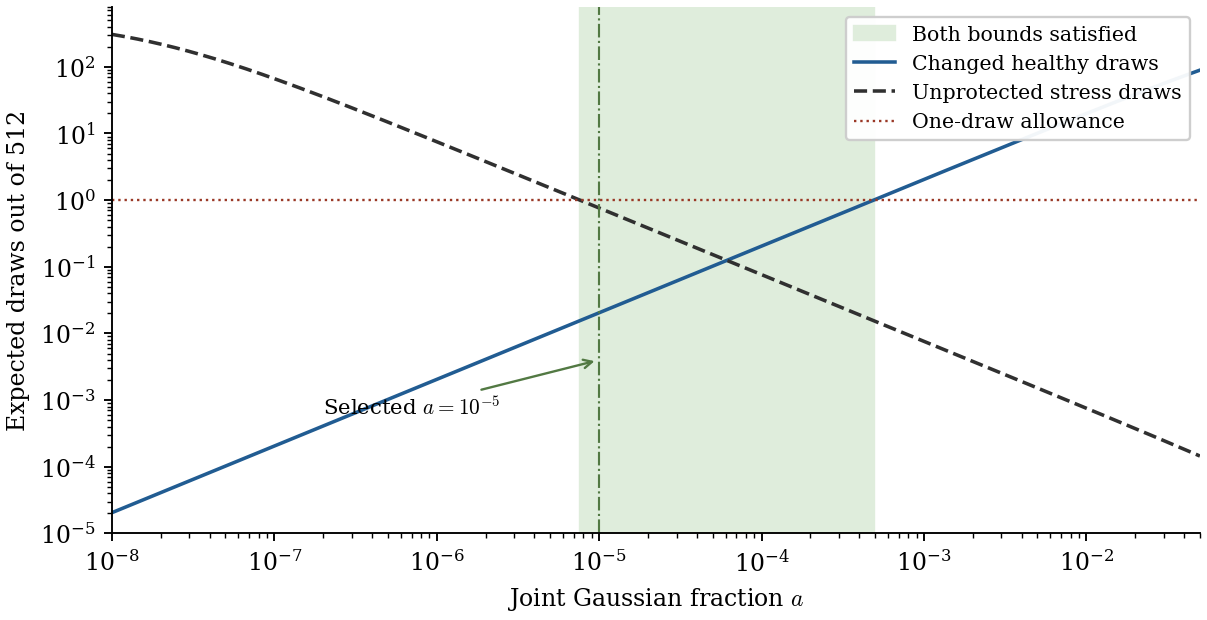
\includegraphics[width=.96\linewidth]{../observation-tt-manuscript-20260915-01/defense-calibration.pdf}
\caption{Both safety requirements can hold simultaneously. The shaded interval
keeps the expected number of changed healthy draws and unprotected stress
draws below one out of 512. The two curves are evaluated at the declared
conditional-mass boundaries; they do not describe nonlinear target coverage.}
\label{fig:sgqf-defense-calibration}
\end{figure}

The compiled sampler passes 96 stress configurations spanning constant and
nonconstant current polynomials, zero conditional mass and amplitude
rescalings. Maximum direct-density disagreement is below $1.43\times10^{-14}$.
These checks establish the stated implementation identities within their
tested scope. They do not make TT fitting reliable: at fixed fitted cores,
fresh-row comparisons still include early cases where SGQF has lower
discrepancy. The next question is consequently downstream. With this small
defense and the option to select the exact Gaussian conditional fixed in
advance, does the complete filter compare favorably on new observation
sequences?

\subsection{An independent filtering comparison}
\label{sec:sgqf-independent-filtering}

The reviewed continuation generated twelve independent observation sequences
in each of $d=1$ and $d=4$, with $T=20$. Each proposal uses 512 particles and
four particle-filter replications. Its eight methods include the transition,
stationary-prior, SGQF marginal and SGQF joint conditionals, alongside the
scalar predictive, scalar guided, pair TT and SGQF-safeguarded pair TT
proposals. The safeguarded method performs its per-observation fitting under
frozen controls and compares generic-start TT, SGQF-start TT and the exact
SGQF joint on validation discrepancy. At time zero it uses SGQF directly.
The selected current marginal enters the next fitting target. No filtering
outcome or audit score changes the frozen fitting or selection rules.

Independent sequences, rather than four repeated particle runs on one
sequence, supply the units for paired uncertainty. The primary error is
mean-squared filtering-mean error normalized by each coordinate's stationary
variance, averaged over the four particle replications. Comparisons are made
overall and for near-zero, ordinary and large coordinate observations, using
$|y_j|/\beta\leq0.5$, $0.5<|y_j|/\beta<2$ and $|y_j|/\beta\geq2$.
One-dimensional references use a grid refinement check; four-dimensional
references use replicated bootstrap filters at increasing particle counts
with declared precision and agreement screens. A regime with insufficient
sequence coverage, or a reference that fails its screen, remains inconclusive.
The sequence bootstrap jointly accounts for the predeclared heuristic
comparisons. A06 required clearing those simple proposals for promotion;
comparisons among the TT variants remain descriptive. A08 retains these
comparisons as performance diagnostics and limits on promotion, while asking
whether the TT proposal supports a useful corrected filter. Lower fit
discrepancy cannot replace that downstream measurement.

The completed candidate fails A06's promotion criterion. In one dimension it has
observed losses to the transition proposal on ordinary observations and to
the analytical SGQF joint conditional on large observations. In four
dimensions the shared SGQF guide fails on one sequence, leaving the complete
comparison unavailable. All twenty-four references nevertheless pass their
declared screens. The scalar grids agree within $7.11\times10^{-16}$
stationary standard deviations for the mean and $7.11\times10^{-15}$ for
log evidence. Nine four-dimensional references use four runs of 65536
particles, and three require the predeclared enlargement to four runs of
131072. Their largest mean MCSE is $0.01735$ stationary standard deviations
and largest log-evidence MCSE is $0.05060$, below limits $0.02$ and $0.10$;
all two-scale agreement checks also pass. These are resolution and Monte
Carlo precision checks, not exactness proofs for the four-dimensional filter.

Table~\ref{tab:sgqf-independent-mse} uses equal sequence weights after
averaging squared errors over particle replications and the relevant
coordinate-time cells within each sequence. Every four-dimensional method
uses the same eleven successful-guide sequences. Their apparently favorable
TT results therefore describe the subset on which the guide succeeds; they
cannot be used to remove its failure from the reliability assessment.

\begin{table}[htbp]
\centering
\small
\begin{tabular}{clrrrr}
\toprule
$d$ & Proposal & All & Near zero & Ordinary & Large\\
\midrule
1 & Transition & 0.0021600 & 0.0030579 & 0.0011964 & 0.0020561\\
1 & Stationary prior & 0.0051131 & 0.0056793 & 0.0018754 & 0.0098854\\
1 & SGQF marginal & 0.0037369 & 0.0049775 & 0.0027870 & 0.0030887\\
1 & SGQF joint & 0.0018482 & 0.0024519 & 0.0014518 & 0.0011200\\
1 & Predictive TT & 0.0015124 & 0.0019170 & 0.0012909 & 0.0007813\\
1 & Guided TT & 0.0016963 & 0.0018042 & 0.0013399 & 0.0017197\\
1 & Original pair TT & 0.0016075 & 0.0017946 & 0.0012691 & 0.0015217\\
1 & SGQF-preserving TT & 0.0016702 & 0.0019506 & 0.0014199 & 0.0013987\\
\midrule
4 & Transition & 0.0066377 & 0.0093457 & 0.0041904 & 0.0065428\\
4 & Stationary prior & 0.0212687 & 0.0279851 & 0.0143865 & 0.0221852\\
4 & SGQF marginal & 0.0060415 & 0.0086580 & 0.0041741 & 0.0039220\\
4 & SGQF joint & 0.0029703 & 0.0034087 & 0.0022337 & 0.0033048\\
4 & Predictive TT & 0.0072739 & 0.0105720 & 0.0052669 & 0.0038474\\
4 & Guided TT & 0.0066699 & 0.0090306 & 0.0053657 & 0.0034635\\
4 & Original pair TT & 0.0026151 & 0.0032617 & 0.0021797 & 0.0020670\\
4 & SGQF-preserving TT & 0.0023614 & 0.0029321 & 0.0019547 & 0.0018882\\
\bottomrule
\end{tabular}
\caption{Normalized filtering-mean MSE on independent sequences. All twelve scalar sequences enter the upper panel. The lower panel uses the same eleven successful-guide sequences for every method; it is descriptive and excludes the guide failure only to make the available comparisons matched. The failure still blocks promotion. These squared, variance-normalized errors differ from the RMSE in Table~\ref{tab:pair-conditional-errors}; they are not a numerical before/after comparison with that earlier exposed sequence.}
\label{tab:sgqf-independent-mse}
\end{table}

For uncertainty, the paired unit is the independent observation sequence.
The 9999 bootstrap resamples retain the dependence between methods and
regimes. Each interval is centered on the observed candidate-minus-heuristic
MSE difference, with half-width equal to the observed sequence standard error
times the 95th percentile of the maximum absolute standardized bootstrap
deviation. Complete, adequately covered contrasts enter this maximum; a
failed comparison receives no interval. All sixteen scalar contrasts qualify,
whereas every four-dimensional contrast is incomplete. The resulting
simultaneous critical value is $2.725897$. At least eight sequences and
twenty-four cells per regime, and a half-width no larger than $0.01$, were
required in advance. Twelve sequences support only an approximate bootstrap
analysis, without a finite-sample coverage guarantee.

The two scalar observed losses are small and not statistically established.
The ordinary-observation difference against transition is $+0.00022344$,
with simultaneous interval from $-0.00018662$ to $0.00063349$. The
large-observation difference against joint SGQF is $+0.00027871$, with
interval from $-0.00050373$ to $0.00106115$. Both intervals include zero. Either positive
observed difference nevertheless blocks advancement under the predeclared
heuristic rule. This distinction prevents a failure to demonstrate
noninferiority from being reported as evidence of inferiority.

Seven scalar intervals have negative upper limits: near-zero observations
against transition; all, near-zero and ordinary observations against the
stationary prior; and the same three groups against the SGQF marginal.
They support only these specified directional comparisons under the
bootstrap assumptions. None of the four contrasts against joint SGQF has a
negative upper limit. Its all-observation difference is $-0.00017804$ with
interval $[-0.00058381,0.00022773]$. The stationary-prior comparison on
large observations also misses the precision requirement, with half-width
$0.010486$. Thus the data do not support an overall ranking, improvement
over joint SGQF, or equivalence in the unresolved regimes.

The four-dimensional failure occurs at zero-based time 18 of sequence 8,
when the observation is approximately
$(-3.1916,2.7754,-0.3507,0.1547)$ and $\beta=0.4$. Every signed
sparse-quadrature level from 2 through 5 estimates positive posterior mass
but an invalid covariance. Their minimum eigenvalues are approximately
$-6.68\times10^{-12}$, $-0.001137$, $-1.08550$ and $-0.080229$.
The Gaussian conditioning formulas remain correct, but they require a
positive-definite covariance that this quadrature calculation does not
supply. The larger negative eigenvalues at the higher levels weaken a
pure roundoff explanation. An unchanged CPU replay reproduces the failure.
No ridge, covariance clipping or replacement proposal was substituted after
seeing the data. Six guide-dependent methods consequently have no complete
result on this sequence, while the two unguided methods finish.

The other particle runs contain no nonfinite stored numerical values or
recorded conditional-CDF bracket failure; the largest recorded inversion
residual is $1.44\times10^{-14}$. These checks support the completed
conditional consumers. They cannot turn the missing guided result into a
successful filter or certify its population accuracy.

The saved fits also clarify what initialization and empirical selection
accomplish. On the 209 four-dimensional transitions with a valid guide,
validation selects the SGQF-started TT 191 times, the generic TT ten times
and the unchanged SGQF joint eight times. In one dimension the corresponding
counts over 228 transitions are 59, 145 and 24. Every initial proposal uses
SGQF. These are decisions along dependent approximate filtering paths, not
independent replications of an initialization comparison.

Although validation selection cannot lose on its own comparison rows,
fresh audit rows reveal losses to SGQF in nine scalar and one
four-dimensional transition fits. The largest increases in $H^2$ are
$0.002248$ and $0.002169$. The finite-row safeguard therefore provides no
population guarantee. Minimum target-weight ESS on the 8192 audit rows is
5859 in one dimension and 985 in four; the four-dimensional validation
minimum is 269 out of 4096. Those concentrations help explain the
uncertainty in selecting a fit. They are not downstream filtering criteria.
The next retained target also depends on the preceding approximation, so
even an accurately measured discrepancy on that target cannot by itself
establish agreement with the true filtering distribution.

There is a measurable computational cost to attempting both fits. In the
same campaign, median fit/total time per sequence is $0.170/0.647$ seconds
for scalar joint SGQF and $5.594/6.593$ for the safeguarded TT. The
four-dimensional values are $0.189/0.665$ and $43.520/45.624$. Shared guide
construction is recorded separately, and the ordered campaign reuses
compiled kernels, so these are descriptive timings rather than an equal
cold-start benchmark.

The experiment withholds promotion of the tested configuration while leaving
two distinguishable repair questions. Signed quadrature must provide valid
moments on the observations where the guide is needed. Separately, TT
conversion and fitting must produce a normalized, evaluable proposal whose
importance corrections permit useful filtering estimates. Discrepancy from
the analytical SGQF joint helps diagnose this second question; any positive
discrepancy difference is not, by itself, a rejection of the TT proposal.
The current observation sequences have now been inspected: a rerun can check
reproducibility and recover missing diagnostics, but a tuned repair requires
fresh confirmation sequences. A lower fitting discrepancy or a favorable
table conditioned on guide success would not answer both questions.

The initialization, defense-calibration and independent-filtering records are
respectively
\path{docs/plans/observation-aware-tt-sgqf-initialization-20260915-result.md},
\path{docs/plans/observation-aware-tt-defense-consumer-20260915-result.md}, and
\path{docs/plans/observation-aware-tt-independent-filtering-20260915-result.md}.
They preserve commands, exact inputs, frozen controls, failed cases and
inference tables. A06's independent terminal interpretation review agreed with
its then-stated promotion and uncertainty limits. This section remains a
provisional manuscript addition pending human reading feedback; its
initialization/selection extensions do not establish source-faithful TT-cross,
scalable high-dimensional fitting, total parameter gradients or HMC readiness.

\subsection{The downstream objective and particle ESS}
\label{sec:tt-downstream-objective}

A08 asks whether the fitted TT is useful in the corrected filtering computation.
Let $q_t(x\mid x_{t-1})$ denote the proposal actually sampled, and let
$w_{t-1}^{(i)}$ be the normalized particle weight carried into the update.
With transition density $f$ and observation density $g$, the implemented
correction for a draw $x_t^{(i)}$ from that proposal is
\begin{align}
 u_t^{(i)} & = w_{t-1}^{(i)}
 \frac{f(x_t^{(i)}\mid x_{t-1}^{(i)})g(y_t\mid x_t^{(i)})}
 {q_t(x_t^{(i)}\mid x_{t-1}^{(i)})},
 & w_t^{(i)}&=\frac{u_t^{(i)}}{\sum_{j=1}^N u_t^{(j)}},\\
 \ESS_t&=\frac{1}{\sum_{i=1}^N(w_t^{(i)})^2},
 &\widehat m_t&=\sum_{i=1}^N w_t^{(i)}x_t^{(i)}.
\end{align}
At the initial observation, the prior density replaces $f$ and the incoming
weights are $1/N$. The sum of unnormalized weights is the evidence increment;
summing its logarithm over time gives the particle log-evidence estimate.
ESS is measured before resampling, which occurs here when $\ESS_t<N/2$.
Equal weights give $\ESS_t=N$, while one dominant weight gives a value near
one. The maximum weight and the number of distinct parents retained by that
resampling step help distinguish typical efficiency from occasional collapse.
They do not measure long-term genealogical diversity.

This ESS concerns actual filtering particles. It differs from the importance
ESS of rows used to fit a TT. It also differs from a validation of the
uncorrected retained TT density: exact importance corrections can yield useful
particle estimates even when the fitted density is imperfect. Accordingly,
the filtering-mean error and log evidence are compared with independent
references, while ESS and weight tails explain the cost of correcting the
proposal. A TT fit need not defeat SGQF on every audit panel for this test to
be informative. No numerical ESS acceptance threshold is chosen after seeing
the result.

The A08 rerun preserves A06's observations, fitting controls and particle
seeds and adds explicit particle-diagnostic summaries. It is a reproducibility
check with additional measurements, not a new independent confirmation.
Moreover, the safeguarded route can select the analytical SGQF joint: its
results describe that selection policy rather than a TT-only recursion.
The pair-TT arm provides a separate comparator without that per-step selection.

The rerun completed on the RTX 5080 in 2023.805 seconds and reproduced the
earlier filtering-error tables and bootstrap intervals exactly. All 24
reference screens passed. The same four-dimensional guide failure left eleven
complete sequences for comparisons involving TT. Across the 14880 completed
particle-time records there were no stored nonfinite numeric values or
recorded conditional-CDF bracket failures. Table~\ref{tab:a08-particle-ess}
reports actual particle ESS alongside filtering error, with the same sequence
denominator for every method within a dimension.

\begin{table}[htbp]
\centering\small
\begin{tabular}{llrrrr}
\toprule
$d$ & Proposal & Norm. MSE & Mean ESS & Min. ESS & Resampled\\
\midrule
1 & Pair TT & 0.0016075 & 379.67 & 76.76 & 7.71\%\\
1 & Selected TT/SGQF & 0.0016702 & 375.82 & 55.98 & 7.50\%\\
\midrule
4 & Transition & 0.0066377 & 175.78 & 2.70 & 79.89\%\\
4 & SGQF joint & 0.0029703 & 311.47 & 3.16 & 30.23\%\\
4 & Scalar guided TT & 0.0066699 & 199.52 & 14.34 & 87.50\%\\
4 & Pair TT & 0.0026151 & 310.55 & 38.77 & 30.00\%\\
4 & Selected TT/SGQF & 0.0023614 & 317.53 & 44.39 & 27.50\%\\
\bottomrule
\end{tabular}
\caption{A08 particle diagnostics, with $N=512$. The scalar panel uses twelve
sequences and the four-dimensional panel uses eleven complete-guide sequences.
ESS is measured before resampling. Minima and resampling frequencies are
descriptive, and no TT-versus-TT ranking is established.}
\label{tab:a08-particle-ess}
\end{table}

For the selected route, the largest normalized particle weights are 0.1064
and 0.1254 in one and four dimensions. Mean log-evidence errors are
$-0.01384$ and $-0.01068$ nats, with largest absolute sequence-mean errors
0.07673 and 0.13624 nats. The four-dimensional MSE is descriptively 64.6\%
below scalar guided TT and 9.7\% below pair TT; the scalar result does not
show the same gain over pair TT. This contrast supports further TT work
without asserting uniform superiority.

The selected policy uses generic TT, SGQF-start TT and exact SGQF at
145, 59 and 36 scalar time steps, and 10, 191 and 19 four-dimensional time
steps. The SGQF counts include the fixed initial steps. Consequently these
results support the utility of a predominantly TT selection policy, while
the stand-alone warm-start TT recursion remains a distinct test. The guide
failure, completion-conditioned four-dimensional comparison and lack of
TT-arm uncertainty intervals remain the main limitations. The two scalar
heuristic losses still have simultaneous intervals containing zero. They
limit the earlier promotion claim; they do not establish that TT is unusable.
The full comparison and per-step records are linked from
\path{docs/plans/observation-aware-tt-downstream-filter-objective-20260916-result.md}.

\section{Stable coordinates and a physical defense against guide collapse}
\label{sec:robust-guide}

The purpose of the Gaussian guide is to make a conditional TT proposal easier
to fit. A failed guide should therefore make approximation less efficient,
not destroy the coordinates in which the proposal is represented. This
distinction matters for the four-dimensional stochastic-volatility example.
In the A09 confirmation sequence s04 at time 8, a nine-node signed sparse
quadrature rule assigned normalized weight essentially one to a single node.
The sum of the other absolute weights was $1.38\,10^{-31}$. Its computed
covariance eigenvalues lay between $3.72\,10^{-32}$ and $2.44\,10^{-31}$,
although the predictive covariance eigenvalues were between 1.20 and 1.32.
All higher tested rules had an indefinite covariance. A check relative to
the candidate covariance's own scale accepted the tiny positive matrix.
Consequently the Gaussian component used to defend the TT polynomial had
the same collapsed physical scale as the fitted TT. The corrected filter
then failed log-evidence agreement, despite apparently valid factorizations.

The highest-resolution particle reference for this sequence had marginal
variances approximately $(1.07,0.25,0.71,0.90)$ at that time. This is strong
diagnostic evidence against interpreting the near-zero guide covariance as
real posterior concentration. It is not a theorem about every small
posterior covariance. The saved replay is
\path{docs/plans/artifacts/observation-tt-warm-improvement-20260916-01/covariance-collapse-diagnostic.md}.
The A09 evidence also exposed seed reuse in earlier attempts; earlier
independence-based Monte Carlo standard errors must not be reused without
their own seed audit. The present construction and its fresh tests are
specified by amendment A10.

We use three protections with different mathematical purposes. First,
quadrature diagnostics reject numerically unresolved Gaussian moments.
Second, model-based TT coordinates remain nonsingular even when those
moments fail. Third, a mixture with the physical transition density gives
the proposal independent tail coverage. None of these statements alone
certifies the accuracy of Gaussian quadrature or the quality of TT fitting.
They define an optional extension of the proposal construction, rather than
a new claim about fidelity to the Zhao--Cui author implementation.

\subsection{What a covariance check can establish}

Let the Gaussian predictive approximation be $p^-(x)=\mathcal N(x;m,S)$,
where $S=LL^\top\succ0$. A quadrature rule has nodes $u_i$ in predictive
standard coordinates and possibly signed weights $w_i$. Put
\begin{equation}
 a_i=w_i\exp\{\ell(m+Lu_i)-b\},\qquad
 A=\sum_i a_i,\qquad b=\max_i\ell(m+Lu_i),\qquad
 \alpha_i=a_i/A .
 \label{eq:robust-signed-weights}
\end{equation}
Here $\ell(x)=\log g(y\mid x)$ and $b$ only prevents numerical overflow.
When $A>0$, the formal quadrature mean and covariance in these coordinates
are $\bar u=\sum_i\alpha_i u_i$ and
$C=\sum_i\alpha_i(u_i-\bar u)(u_i-\bar u)^\top$.
The physical moments are $m+L\bar u$ and $LCL^\top$. These formulas are
quadrature estimates; signed $\alpha_i$ are not probabilities.

\begin{proposition}[A relative SPD test does not protect physical scale]
\label{prop:robust-scale}
For any $c\in(0,1)$, the test
$\lambda_{\min}(C)>c\|C\|_2$ accepts every $C=\delta I_d$ with
$\delta>0$, however small $\delta$ is relative to a predictive covariance.
Moreover, positive normalized quadrature weights do not prevent their
weighted covariance from converging to zero.
\end{proposition}
\begin{proof}
For $C=\delta I_d$, both $\lambda_{\min}(C)$ and $\|C\|_2$ equal
$\delta$, so the inequality reduces to $1>c$. For the second assertion,
fix finitely many nodes and let the weight of one node tend to one while
all other nonnegative weights tend to zero. The weighted mean tends to that
node, and every term in the finite covariance sum tends to zero.
Thus positivity prevents an indefinite exact weighted covariance but does
not prevent concentration on a single quadrature node.
\end{proof}

There are two distinct numerical warnings. Cancellation is measured by
$\kappa_A=\sum_i|a_i|/|A|$; dominance is measured by
$D_A=\max_i|a_i|/\sum_i|a_i|$. The latter uses absolute weights and
remains meaningful for a signed rule. It is not an effective sample size.

\begin{proposition}[Cancellation and moment sensitivity]
\label{prop:robust-cancellation}
Suppose the summands $a_i$ are exact, their floating-point sum is computed
without overflow or underflow, and $n\epsilon_{\rm mach}<1$. In the
usual rounding model its absolute error is at most
$\gamma_n\sum_i|a_i|$, where
$\gamma_n=n\epsilon_{\rm mach}/(1-n\epsilon_{\rm mach})$.
Hence the relative error bound is $\gamma_n\kappa_A$ when $A\ne0$.
In exact arithmetic a signed normalized weighted covariance can be
indefinite even when $A>0$; this is a separate failure from cancellation.
\end{proposition}
\begin{proof}
Expanding successive rounded additions gives
$\widehat A=\sum_i a_i(1+\theta_i)$ with
$|\theta_i|\le\gamma_n$. The triangle inequality proves the absolute
bound, and division by $|A|$ proves the relative bound. The same argument
applies entry by entry to sums defining moments, with the appropriate
absolute summands. It does not account for errors in evaluating likelihoods
or centered nodes. For indefiniteness, the one-dimensional nodes $0,1$
with normalized weights $2,-1$ have mean $-1$ and variance
$2(0+1)^2-(1+1)^2=-2$. Their total weight is one.
\end{proof}

We therefore evaluate covariance in predictive units and compare its
smallest eigenvalue with a margin that has an independent unit scale:
\begin{equation}
 \eta_C=64\epsilon_{\rm mach} n
 \max\!\left\{1,\sum_i |\alpha_i|\|u_i-\bar u\|^2\right\},
 \qquad \lambda_{\min}(C)>\eta_C .
 \label{eq:robust-margin}
\end{equation}
Finite values, positive signed mass and a corresponding cancellation check
are also required. The factor 64 is a conservative numerical hypothesis,
not a proved forward-error constant for the whole algorithm. This check
rejects numerically unusable guide moments; it does not assert that a true
posterior cannot be concentrated. No eigenvalue is clipped and no hidden
ridge is added to accepted moments. Dominance, cancellation, eigenvalues
and standardized third and fourth moments are retained as diagnostics.

Numerical admissibility is followed by a resolution check. Successive
admissible rules must agree in mean, covariance and log integral to declared
tolerances: $0.02$ predictive standard-deviation units for the Euclidean
mean difference, $0.05$ for the relative Frobenius covariance difference,
and $0.02$ nats for the log integral. The covariance denominator is the
larger of one and the earlier covariance's Frobenius norm in predictive
units. Agreement of two rules is evidence of resolution at those orders,
not a quadrature error bound: both rules can miss the same mass. A failed
check triggers the following independent construction.

\subsection{An observation-adapted positive quadrature repair}

In the example, $x,m\in\mathbb R^d$, $S\in\mathbb R^{d\times d}$ is
symmetric positive definite and therefore invertible, $\beta>0$, and,
conditionally on $x$,
$y_j$ are independent $\mathcal N(0,\beta^2 e^{x_j})$ variables. Combining
this likelihood with the Gaussian predictive approximation gives the
negative log density, up to a constant independent of $x$,
\begin{equation}
 U(x)=\tfrac12(x-m)^\top S^{-1}(x-m)
       +\tfrac12\sum_{j=1}^d\{x_j+c_j e^{-x_j}\},
 \qquad c_j=(y_j/\beta)^2\ge0 .
 \label{eq:robust-sv-potential}
\end{equation}
This is a density for the Gaussian-predictive approximation. It equals
neither the full filtering density in general nor a TT-retained target.

\begin{proposition}[Unique mode of the Gaussian-predictive SV update]
\label{prop:robust-mode}
If $S\succ0$, $\beta>0$ and all $y_j$ are finite, $U$ is coercive and
strongly convex. It has a unique minimizer $x_*$, with
\begin{align}
 \nabla U(x)&=S^{-1}(x-m)+\tfrac12(\boldsymbol1-c\odot e^{-x}),
 \nonumber\\
 H(x)&=S^{-1}+\tfrac12\operatorname{diag}(c\odot e^{-x})\succ0 .
 \label{eq:robust-mode-derivatives}
\end{align}
The mode is a smooth function locally of $(m,S,y,\beta)$ on the domain
$S\succ0$, $\beta>0$, including observations with zero components.
\end{proposition}
\begin{proof}
Differentiating \eqref{eq:robust-sv-potential} gives the displayed gradient
and Hessian. The diagonal addition is positive semidefinite, so
$H(x)\succeq S^{-1}\succeq\lambda_{\min}(S^{-1})I$ for all $x$.
The quadratic term dominates the possibly negative linear term as
$\|x\|\to\infty$, while the exponential term is nonnegative. This
proves coercivity, existence and uniqueness. The gradient is smooth in all
parameters on the stated open domain. Its derivative with respect to $x$
at the solution is the invertible Hessian. The implicit function theorem
gives the local smooth dependence. Setting a $y_j$ to zero leaves these
arguments unchanged.
\end{proof}

We solve for the mode with damped Newton steps and a backtracking decrease
test using the displayed analytical derivatives. A finite residual check
is required before using $V=H(x_*)^{-1}$. The proposition concerns the
exact mode; it does not prove that any fixed numerical iteration budget
will attain its tolerance. Failed factorizations or unresolved residuals
are recorded rather than concealed by covariance clipping.

Let $q_L(x)=\mathcal N(x;x_*,V)$ and write $x=x_*+Bu$, where
$BB^\top=V$ and $u$ has standard Gaussian density $\rho$.

\begin{proposition}[Positive quadrature with the correct density ratio]
\label{prop:robust-change-measure}
For any function $h$ integrable under $p^-(x)g(y\mid x)$,
\begin{equation}
 \int h(x)p^-(x)g(y\mid x)\,dx
 =\int h(x_*+Bu)
   \frac{p^-(x_*+Bu)g(y\mid x_*+Bu)}{q_L(x_*+Bu)}\rho(u)\,du .
 \label{eq:robust-change-measure}
\end{equation}
A positive Gauss--Hermite rule for the right-hand side produces positive
normalized weights. With strictly positive finite likelihood ratios and
nodes whose physical locations affinely span $\mathbb R^d$, its exact
weighted covariance is positive definite. Neither assertion establishes
the accuracy or numerical conditioning of the finite quadrature rule.
\end{proposition}
\begin{proof}
The substitution has Jacobian $|\det B|$, and
$q_L(x_*+Bu)|\det B|=\rho(u)$. Substitution proves the identity and
shows why the predictive-to-Laplace density ratio cannot be omitted.
Multiplying positive quadrature weights by a positive likelihood ratio
preserves positivity. For normalized weights $\omega_i>0$ and any
$v\ne0$, the weighted variance is
$\sum_i\omega_i[v^\top(x_i-\bar x)]^2$. It vanishes only if
$v^\top x_i$ is constant at every node. Affine spanning excludes this
possibility. Proposition~\ref{prop:robust-scale} still permits arbitrarily
small variances when almost all weight is concentrated at one node.
\end{proof}

A10 tests tensor orders 5, 7 and 9, at most $9^4=6561$ nodes, using
log-sum-exp normalization and the same numerical and resolution diagnostics.
The small-dimensional tensor rule is a bounded repair experiment; its
exponential growth prevents a claim of a scalable high-dimensional
implementation. It is not the generic all-axes retained-grid Zhao--Cui
route. If neither signed sparse quadrature nor this repair resolves the
guide, the predictive Gaussian is used explicitly as an unresolved-guide
fallback. This preserves a usable proposal but supplies no observation
adaptation at that step.

\subsection{TT coordinates that do not inherit guide covariance collapse}

Let the physical dynamics be $x_t=A x_{t-1}+\xi_t$, with
$\xi_t\sim\mathcal N(0,Q)$, $Q\succ0$, and initial covariance
$P_0\succ0$. Define deterministic model covariances
\begin{equation}
 R_0=P_0,\qquad R_t=A R_{t-1}A^\top+Q,\qquad
 x_t=c_t+L_t u_t,\quad L_tL_t^\top=R_t .
 \label{eq:robust-chart}
\end{equation}
The center $c_t$ may be the accepted or repaired guide mean. The covariance
$R_t$ is independent of the guide's observation-weighted covariance. In the
stationary fixture, $A P_0A^\top+Q=P_0$ and $R_t=P_0$ for every $t$.

\begin{proposition}[A nonsingular chart and invariant physical proposals]
\label{prop:robust-chart}
For finite $t$, finite $A,Q,P_0$ satisfying the assumptions above,
$R_t\succ0$ and $R_t\succeq Q$ for $t\ge1$.
The affine change of coordinates is bijective. If a physical density $p$
is represented in these coordinates as
$p_U(u)=p(c_t+L_tu)|\det L_t|$, then its physical law is unchanged.
The same statement holds for a joint law after transforming both states.
\end{proposition}
\begin{proof}
For nonzero $v$,
$v^\top R_tv=(A^\top v)^\top R_{t-1}(A^\top v)+v^\top Q>0$;
induction starts from $P_0\succ0$. The first summand is nonnegative, which
also proves $R_t\succeq Q$. Every finite recursion has finite entries in
exact real arithmetic, and its Cholesky factor is nonsingular. The
change-of-variables formula gives the asserted density, with determinant
$|\det L_t|$; a block-diagonal affine transformation gives the joint
version. Centering translates the coordinates and does not change the
factor's singular values.
\end{proof}

This proposition removes guide collapse as a source of chart singularity.
It does not bound $R_t$ uniformly for unstable dynamics, guarantee safe
floating-point arithmetic for arbitrary $A,Q$, or imply that a low-degree
TT fits well in the broader coordinates. Numerical factorizations are still
checked. In particular, Gaussian initialization and regression sampling must
transform the same physical SGQF joint into the new charts. Reinterpreting
$R_t$ as the guide covariance would instead change the initializer and
the design distribution. The implementation checks this distinction at the
consumer endpoint, not just inside a coordinate utility.

For clarity, let the incoming guide be $\mathcal N(m_z,P_z)$, the current
guide be $\mathcal N(m_x,P_x)$, and define
$S_z=A P_zA^\top+Q$, $K=P_zA^\top S_z^{-1}$ and
$B_z=P_z-KS_zK^\top$. The Gaussian joint used for initialization has
\begin{equation}
 \begin{pmatrix}x\\z\end{pmatrix}\sim\mathcal N\!\left(
 \begin{pmatrix}m_x\\m_z+K(m_x-Am_z)\end{pmatrix},
 \begin{pmatrix}P_x&P_xK^\top\\KP_x&B_z+KP_xK^\top\end{pmatrix}
 \right).
 \label{eq:robust-initializer-joint}
\end{equation}
This follows by drawing $x$ from the current guide and then drawing
$z\mid x\sim\mathcal N(m_z+K(x-Am_z),B_z)$; conditional expectation
and the law of total covariance give every block. Equation
\eqref{eq:robust-chart} transforms this joint without substituting $R_t$
for either $P_x$ or $P_z$.

\subsection{A defensive component in physical coordinates}

Let $q_{\rm TT}(x\mid z)$ be the normalized conditional proposal obtained
from the fitted pair TT, including its internal polynomial-zero defense.
That internal component is Gaussian in the TT chart. Define instead the
additional physical mixture
\begin{equation}
 q_\varepsilon(x\mid z)
 =(1-\varepsilon)q_{\rm TT}(x\mid z)
       +\varepsilon f(x\mid z),\qquad 0<\varepsilon<1,
 \quad f(x\mid z)=\mathcal N(x;Az,Q).
 \label{eq:robust-mixture}
\end{equation}
At time zero the second component is the physical prior. A component label
is sampled with probabilities $1-\varepsilon,\varepsilon$, followed by a
draw from that component. Both component densities must then be evaluated
at the actual sampled point. Using only the sampled component's density in
the denominator implements a different importance calculation.

\begin{proposition}[Normalization and exact conditional importance correction]
\label{prop:robust-mixture-correction}
Suppose $q_{\rm TT}(\cdot\mid z)$ is a probability density and
$Z_y(z)=\int f(x\mid z)g(y\mid x)\,dx\in(0,\infty)$.
Then \eqref{eq:robust-mixture} is a probability density with
$q_\varepsilon\ge\varepsilon f$. For every integrable $h$,
\begin{equation}
 \mathbb E_{q_\varepsilon}\!\left[
 h(X)\frac{f(X\mid z)g(y\mid X)}{q_\varepsilon(X\mid z)}\right]
 =\int h(x)f(x\mid z)g(y\mid x)\,dx .
 \label{eq:robust-importance}
\end{equation}
Thus the exact importance target is unchanged by this proposal mixture.
\end{proposition}
\begin{proof}
Integration of the convex combination gives one, and nonnegativity gives
the lower bound. Multiplying the integrand on the left by its sampling
density cancels the denominator. Since $f$ is everywhere positive, the
mixture covers the target support. Integrability permits the expectation.
\end{proof}

The equality is for unnormalized importance integrals conditional on $z$.
It does not make a finite-sample self-normalized mean unbiased, nor does it
validate a TT approximation's own normalizing constant. In the particle
filter the usual previous particle weights and the declared resampling law
remain part of the calculation.

\begin{proposition}[Finite conditional second moment for the SV likelihood]
\label{prop:robust-second-moment}
Under the SV likelihood above, finite $z,y$, $\beta>0$ and $Q\succ0$,
the importance weight $W=f(X\mid z)g(y\mid X)/q_\varepsilon(X\mid z)$
has finite conditional second moment. In particular, with $\mu=Az$,
\begin{equation}
 \mathbb E_{q_\varepsilon}[W^2\mid z]
 \le \frac{1}{\varepsilon}\mathbb E_{f(\cdot\mid z)}[g(y\mid X)^2]
 \le \frac{(2\pi\beta^2)^{-d}}{\varepsilon}
 \exp\!\left\{-\boldsymbol1^\top\mu
                  +\tfrac12\boldsymbol1^\top Q\boldsymbol1\right\}.
 \label{eq:robust-second-moment}
\end{equation}
The normalized conditional importance ratio $W/Z_y(z)$ also has finite
second moment. This is a pointwise-in-$(y,z)$ assertion, not a uniform ESS
bound or a lower bound on any realized finite-particle ESS.
\end{proposition}
\begin{proof}
Since $q_\varepsilon\ge\varepsilon f$,
$\int f^2g^2/q_\varepsilon\le\varepsilon^{-1}\int fg^2$.
Squaring the likelihood gives
\[
 g(y\mid x)^2=(2\pi\beta^2)^{-d}
 \exp\!\left\{-\boldsymbol1^\top x-\sum_j c_j e^{-x_j}\right\}
 \le (2\pi\beta^2)^{-d}e^{-\boldsymbol1^\top x}.
\]
The Gaussian moment-generating function at $-\boldsymbol1$ gives the
second bound. The same bound, or Cauchy--Schwarz, makes $Z_y(z)$ finite;
strict positivity of the likelihood and transition makes it positive.
Division by its square proves the normalized assertion. It may be very
small, so this argument supplies no useful universal numerical bound on
the normalized variance. At time zero the proof is identical with the
prior mean and covariance replacing $\mu,Q$.
\end{proof}

The first inequality bounds the second moment by $1/\varepsilon$ times
that of the transition proposal. A10 evaluates $\varepsilon=0.05,0.2,0.5$,
whose multipliers are 20, 5 and 2. These are declared robustness/cost
hypotheses. They do not predict which setting has the smallest filtering
error. The smallest setting passing the calibration safety/non-harm checks
is frozen before fresh confirmation. Runtime switching based on heldout
performance is excluded.

\subsection{Differentiability and the remaining empirical question}

\begin{proposition}[Smooth mixture density on a fixed branch]
\label{prop:robust-smoothness}
Let $\vartheta$ collect continuous state or model parameters. On an open
domain suppose $q_{\rm TT}(x\mid z;\vartheta)$ and
$f(x\mid z;\vartheta)$ are positive $C^1$ densities and $\varepsilon$
is a fixed number in $(0,1)$. Then $\log q_\varepsilon$ is $C^1$, with
\begin{equation}
 \nabla_\vartheta\log q_\varepsilon
 =r_{\rm TT}\nabla_\vartheta\log q_{\rm TT}
   +r_f\nabla_\vartheta\log f,\qquad
 r_{\rm TT}=\frac{(1-\varepsilon)q_{\rm TT}}{q_\varepsilon},
 \quad r_f=\frac{\varepsilon f}{q_\varepsilon}.
 \label{eq:robust-mixture-score}
\end{equation}
This statement alone gives no derivative of adaptive guide selection,
TT fitting, component selection or particle resampling.
\end{proposition}
\begin{proof}
A fixed positive convex combination of $C^1$ functions is positive and
$C^1$. Differentiating its logarithm and multiplying and dividing each
summand by its positive component density gives the formula. The argument
treats the component densities as differentiable functions on the stated
domain; it does not differentiate any algorithm used to select or construct
them. Branch changes, active-set changes in L1 fitting, singular-value
choices and discrete resampling therefore require additional analysis.
\end{proof}

The proposal remains analytically differentiable in its evaluation
coordinates when its fitted cores and positive charts are held fixed. A
total analytical derivative of the complete finite filtering program is a
separate, unproved requirement. The immediate empirical question is more
limited: do the numerical guards detect the observed failure, do the new
charts and physical defense preserve valid filtering on fresh sequences,
and is the cost acceptable? Tests retain quadrature failures, normalized
filtering MSE, log-evidence agreement, particle ESS, maximum weights,
ancestry and timing. Loss against a Gaussian joint describes approximation
quality; it cannot by itself decide whether a TT proposal is useful after
exact importance correction.

\subsection{A10 evaluation of the repair}

The experiment separates three changes. The \emph{guide} arm replaces the
unchecked SGQF moments with the resolution-checked guide while retaining
guide-covariance TT coordinates. The \emph{stable} arm additionally uses
the independent covariance recursion in Proposition~\ref{prop:robust-chart}.
The \emph{full} arm adds the physical transition mixture to that same
stable-coordinate TT. All are compared with the A09 SGQF-initialized pair
TT under the same exact importance correction. Transition, stationary-prior,
SGQF marginal and SGQF joint proposals provide cheap filtering comparisons.
The initial proposal is an analytic Gaussian; subsequent times have separate
TT fits. The stability change therefore does not assert that every proposal,
including the initial Gaussian, has a TT representation.

Calibration uses three independent sequences in each of dimensions one and
four, each of length 20, with four particle repetitions and 512 particles.
It considers L1 weights $10^{-5}$ and $10^{-3}$ and external mixture weights
$0.05,0.2,0.5$. A candidate must retain all three reference-valid sequences;
missing or invalid cases cannot improve its selection score. The smallest
mixture weight satisfying the declared non-harm screen is selected. The
frozen guide L1 weights are $10^{-5}$ in dimension one and $10^{-3}$ in
dimension four; both stable arms use $10^{-3}$. Both dimensions select
$\varepsilon=0.05$. Twelve fresh sequences per dimension then test those
frozen choices, using seed blocks disjoint from calibration.

For sequence $i$, method $a$, repetition $r$ and time $t$, let
$\widehat m^{a}_{irt,j}$ be coordinate $j$ of the estimated filtering mean
and $m^{\rm ref}_{it,j}$ the independent reference mean. With $R=4$, $T=20$
and prior covariance $P_0$, the sequence error is
\[
 M_i^a=\frac{1}{RTd}\sum_{r=1}^R\sum_{t=1}^T\sum_{j=1}^d
 \frac{(\widehat m^a_{irt,j}-m^{\rm ref}_{it,j})^2}{(P_0)_{jj}}.
\]
This measures error against the reference approximation, whose precision is
checked separately. The scalar reference uses nested physical-space grids;
the four-dimensional reference uses transition particle filters with
$32768$, $65536$ and $131072$ particles. Its declared mean-MCSE, log-evidence
MCSE and resolution screens remain active. Observation-coordinate regimes
are $|y_j|/\beta\le0.5$, $0.5<|y_j|/\beta<2$, and $|y_j|/\beta\ge2$.

The paired non-harm statistic is the average of
$M_i^a-1.1M_i^{\rm A09}$. The predeclared sequence bootstrap uses 9999
resamples and simultaneous Bonferroni percentile intervals for the six
dimension-by-repair contrasts. An upper endpoint at most zero supports the
declared 10\% non-harm statement on this experiment. An upper endpoint below
zero for $M_i^a-M_i^{\rm A09}$ supports a reduction under the same exploratory
bootstrap analysis. Twelve sequences provide limited information about
rare failures and tails; neither outcome establishes a universal ranking.
All numerical and reference checks must pass before interpreting a paired
contrast. Conditional losses against the cheap proposals block promotion
under the stated comparison rule; they do not invalidate the TT research
direction or the exact-importance identity.

The confirmation exposed one fitting guard that is separate from these
statistical criteria. Let $h_i$ be the initial TT amplitude evaluated on
training rows, let $b_i$ be the target amplitude and let $w_i\ge0$. The
least-squares scalar is
\begin{equation}
 c^*=\frac{\sum_i w_i h_i b_i}{\sum_i w_i h_i^2}.
 \label{eq:robust-amplitude-scale}
\end{equation}
\begin{proposition}[Amplitude sign is not a density validity condition]
\label{prop:robust-amplitude-sign}
Suppose the denominator in~\eqref{eq:robust-amplitude-scale} is finite and
strictly positive, and $c^*$ is finite and nonzero. Replacing $h$ by
$c^*h$ is valid even when $c^*<0$. If the represented TT density is the
normalized square $q_h(x)=h(x)^2/\int h(u)^2\,du$, then
$q_{c^*h}=q_h$. A zero or nonfinite denominator or scalar remains invalid.
\end{proposition}
\begin{proof}
The stated conditions make the weighted quadratic objective finite and give
its unique scalar minimizer by differentiating
$\sum_iw_i(c h_i-b_i)^2$. A negative minimizer is therefore a valid
least-squares solution. For every $x$,
$(c^*h(x))^2=(c^*)^2h(x)^2$; the same positive factor multiplies the
normalizing integral and cancels. The denominator condition excludes a zero
initial amplitude in the training norm, and finiteness and nonzeroness of
$c^*$ exclude a nonfinite or identically zero initialization. Thus an
assertion $c^*>0$ would reject a valid representation solely because of an
unidentified global amplitude sign. This proof does not justify clipping,
changing the target, or accepting a zero scale.
\end{proof}

The implementation now checks the denominator, finiteness and $|c^*|>0$ and
retains the signed scalar. Positive-scale cases are unchanged to roundoff.
Confirmation-01 d4-s05 had $c^*=-0.3106276393$ and is preserved as the
repair trigger; it is excluded from matched stable/full summaries until a
fresh run evaluates the repaired endpoint.


\appendix
\section{Artifact Provenance and Corrections}

Numerical values were checked in
\path{docs/benchmarks/artifacts/c2_completion_20260824/attempt05/} against:
\begin{itemize}
\item \path{cell_n4_d6_r6_s42_w32.json};
\item \path{reference_n4_s42.json};
\item \path{reference_n4_s142.json};
\item \path{reference_n4_s242.json};
\item the instrumented T=20 diagnostic used by the 2026-08-28 addendum; and
\item \path{n4_failure_independent_review_for_claude_20260828.md}.
\end{itemize}

The instrumented T=20 run was bit-identical to the baseline after its Class-A
observability fields were added. Its Gram statistics begin at $t=1$; no $t=0$
Gram minimum should be inferred. This revised report supersedes the causal
interpretations in \path{n4_diagnostic_handoff_memo_20260828.md} and
\path{n4_diagnostic_t20_result_addendum_20260828.md}; correction notices in
those files preserve their historical text while preventing reuse of the
rejected diagnosis.

\end{document}
